\chapter{The \acl Algorithm} \label{sect:acl}
We now present our proposed \fullacl (\acl) algorithm for the strictly
sequential setting with explicit thresholds.
\acl is similar in spirit to the \gpucb~\cite{srinivas10}
bandit optimization algorithm in that it uses a GP to model the
underlying function and facilitates the inferred mean and variance of the GP
to guide the selection of points to be evaluated.

More concretely, the inferred mean and variance of \eqtref{eq:mean}
and \eqtref{eq:var} can be used to construct a \emph{confidence interval}
\begin{align*}
Q_t(\*x) = \left[\mu_{t-1}(\*x) \pm \beta_t^{1/2}\sigma_{t-1}(\*x)\right]
\end{align*}
for any point $\*x \in D$, which captures our uncertainty about $f(\*x)$
after having already obtained noisy evaluations of $f$ at points
$\{\*x_1,\ldots,\*x_t\}$. The parameter $\beta_t$ acts as a scaling factor
and its choice is discussed later.
The above-defined confidence intervals serve two purposes in our algorithm:
first, they allow us to judge whether a point can be classified into
the super- or sublevel sets or whether the decision should be deferred
until more information is available; second, they guide the sampling
process towards points that are likely to be informative with respect
to the desired level set.

The pseudocode of \algoref{alg:acl} depicts in detail the operation of \acl.
Our algorithm maintains a set of yet unclassified
points $U_t$, as well as a superlevel set $H_t$ and a sublevel set
$L_t$, which are updated at each iteration. Furthermore, the algorithm
maintains for each unclassified $\*x$ a monotonically decreasing
\emph{confidence region} $C_t(\*x)$, which results from intersecting
successive confidence intervals, i.e.
\begin{align*}
C_t(\*x) = \bigcap_{i=1}^t Q_i(\*x) = C_{t-1}(\*x) \cap Q_t(\*x).
\end{align*}
Initially, all points
$\*x \in D$ are unclassified and the confidence regions have infinite
range (\linesref{lin:init1}{lin:init2}). At each iteration, the confidence
regions of all
unclassified points are updated (\lineref{lin:upd}) and each of these points
is either classified into one of $H_t$ or $L_t$, or is left unclassified
(\linesref{lin:class1}{lin:class2}). Then, the next point is selected and
evaluated (\linesref{lin:sel1}{lin:sel2}) and the new GP posterior is
computed (\lineref{lin:inf}) taking into account the newest measurement,
according to equations \eqtref{eq:mean} and \eqtref{eq:var}.
The algorithm terminates when all points in $D$ have been
classified, at which point the estimated super- and sublevel sets
$\hat{H}$ and $\hat{L}$ are returned (\linesref{lin:ret1}{lin:ret2}).

\begin{algorithm}[tb]
  \caption{The \acl algorithm}
  \label{alg:acl}
\small{
\begin{algorithmic}[1]
  \REQUIRE sample set $D$, GP prior ($\mu_0 = 0$, $k$, $\sigma_0$),\\
           \hspace{1.6em}threshold value $h$, accuracy parameter $\epsilon$
  \ENSURE predicted sets $\hat{H}$, $\hat{L}$
  \LET{$H_0$}{$\varnothing$} \label{lin:init1}
  \LET{$L_0$}{$\varnothing$}
  \LET{$U_0$}{$D$}
  \LET{$C_0(\*x)$}{$\mathbb{R}$, for all $\*x \in D$} \label{lin:init2}
  \LET{$t$}{1}
  \WHILE{$U_{t-1} \neq \varnothing$}
    \LET{$H_t$}{$H_{t-1}$}
    \LET{$L_t$}{$L_{t-1}$}
    \LET{$U_t$}{$U_{t-1}$} 
    \FORALL{$\*x \in U_{t-1}$}
      \LET{$C_{t}(\*x)$}{$C_{t-1}(\*x) \cap Q_t(\*x)$} \label{lin:upd}
      \IF{$\min(C_t(\*x)) + \epsilon > h$} \label{lin:class1}
        \LET{$U_t$}{$U_t \setminus \{\*x\}$}
        \LET{$H_t$}{$H_t \cup \{\*x\}$} 
      \ELSIF{$\max(C_t(\*x)) - \epsilon \leq h$} \label{lin:classr2}
        \LET{$U_t$}{$U_t \setminus \{\*x\}$}
        \LET{$L_t$}{$L_t \cup \{\*x\}$}
      \ENDIF \label{lin:class2}
    \ENDFOR
    \LET{$\*x_t$}{$\argmax_{\*x \in U_t}(a_t(\*x))$} \label{lin:sel1}
    \LET{$y_t$}{$f(\*x_t) + \nu_t$} \label{lin:sel2}
    \STATE Compute $\mu_t(\*x)$ and $\sigma_t(\*x)$, for all $\*x \in U_t$ \label{lin:inf}
    \LET{$t$}{$t + 1$}
  \ENDWHILE
  \LET{$\hat{H}$}{$H_{t-1}$} \label{lin:ret1}
  \LET{$\hat{L}$}{$L_{t-1}$} \label{lin:ret2}
\end{algorithmic}
}
\end{algorithm}

We now discuss in more detail the issues of how points are classified and
how the next point to be evaluated is selected at each step.

\section{Algorithm details}

\paragraph{Classification}
The classification of a point $\*x$ into $H_t$ or $L_t$ depends on the
position of its confidence region with respect to the threshold level $h$.
Intuitively, if all of $C_t(\*x)$ lies above $h$, then with high probability
$f(\*x) > h$ and $\*x$ should be moved into $H_t$. Similarly, if $C_t(\*x)$
lies below $h$, then $\*x$ should be moved into $L_t$. Otherwise, we are
still uncertain about the class of $\*x$, therefore it should, for the moment,
remain unclassified. As can be seen in the classification rules
of~\linsref{lin:class1} and~\ref{lin:classr2}, we relax these conditions by
introducing an accuracy parameter $\epsilon$, which
trades off classification accuracy for sampling cost. The resulting
classification scheme is illustrated by the example of \figref{fig:conf},
in which point $\*x$ would be
classified into $H_t$ and point $\*x''$ into $L_t$, while point $\*x'$ would
remain in $U_t$ as unclassified. Note that \acl uses a monotonic
classification scheme, meaning that once a point has been classified, it
stays so until the algorithm terminates.

\begin{figure}[tb]
  \begin{subfigure}[b]{0.49\linewidth}
    \centering
    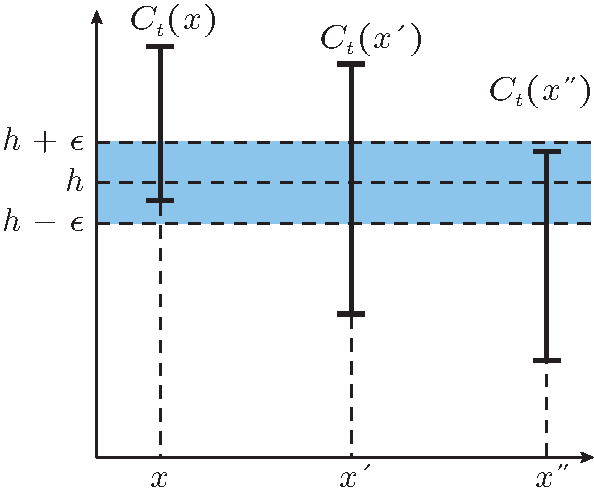
\includegraphics[height=1.5in]{figures/class}
    \caption{Confidence regions}
    \label{fig:conf}
  \end{subfigure}
  \hfill
  \begin{subfigure}[b]{0.49\linewidth}
    \centering
    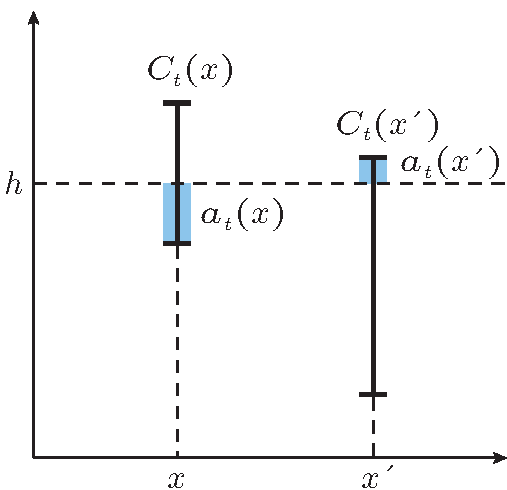
\includegraphics[height=1.5in]{figures/amb}
    \caption{Ambiguities}
    \label{fig:amb}
  \end{subfigure}
  \caption{
    (a) Example of the three possible configurations of confidence regions.
    (b) Ambiguities (shaded) of two example points.
  }
\end{figure}

\paragraph{Sample selection}
For selecting the next point to be evaluated at each iteration, we define the
following quantity
\begin{align*}
a_t(\*x) = \min\{\max(C_t(\*x)) - h, h - \min(C_t(\*x))\},
\end{align*}
which we call classification \emph{ambiguity}. As its name suggests, the
ambiguity of a point $\*x$ quantifies our uncertainty about whether $\*x$
belongs to $H_t$ or $L_t$ (see \figref{fig:amb}).
The intuition of sampling at areas of the sample space with large
classification uncertainty, expecting to gain more information about
the problem at hand when sampling at those areas, manifests itself in \acl
by choosing to evaluate at each iteration the point with the largest
ambiguity amongst the yet unclassified.

We can make an interesting observation at this point. If we use the confidence
intervals $Q_t(\*x)$ instead of the confidence regions $C_t(\*x)$
in the definition of ambiguity, we get the following quantity
\begin{align*}
a'_t(\*x) &= \min\{\max(Q_t(\*x)) - h, h - \min(Q_t(\*x))\}\\
          &= \min\{\mu_{t-1}(\*x) + \beta_t^{1/2}\sigma_{t-1}(\*x) - h,\ h - \mu_{t-1}(\*x) + \beta_t^{1/2}\sigma_{t-1}(\*x)\}\\
          &= \beta_t^{1/2}\sigma_{t-1}(\*x) - |\mu_{t-1}(\*x) - h|.
\end{align*}
For $\beta_t^{1/2} = 1.96$, this is identical to
the \emph{straddle}~\cite{bryan05} heuristic, which can thus be
intuitively explained in terms of classification ambiguity.

%\setlength\figureheight{1.5in}\setlength\figurewidth{2.5in}
%% This file was created by matlab2tikz v0.2.3.
% Copyright (c) 2008--2012, Nico Schlömer <nico.schloemer@gmail.com>
% All rights reserved.
% 
% 
%

\definecolor{locol}{rgb}{0.26, 0.45, 0.65}

\begin{tikzpicture}

\begin{axis}[%
tick label style={font=\tiny},
label style={font=\tiny},
xlabel shift={-10pt},
ylabel shift={-17pt},
legend style={font=\tiny},
view={0}{90},
width=\figurewidth,
height=\figureheight,
scale only axis,
xmin=0, xmax=1478,
xtick={0, 400, 1000, 1400},
xlabel={Length (m)},
ymin=-18, ymax=0,
ytick={0, -4, -14, -18},
ylabel={Depth (m)},
name=plot1,
axis lines*=box,
tickwidth=0.1cm,
clip=false
]

\addplot [fill=locol,draw=none,forget plot] coordinates{ (1478,0)(1478,-0.181818181818182)(1478,-0.363636363636364)(1478,-0.545454545454545)(1478,-0.727272727272727)(1478,-0.909090909090909)(1478,-1.09090909090909)(1478.0002488174,-1.27272727272727)(1478.00049762651,-1.45454545454545)(1478.00074642733,-1.63636363636364)(1478.00074642733,-1.81818181818182)(1478.00074642733,-2)(1478.00074642733,-2.18181818181818)(1478.00074642733,-2.36363636363636)(1478.00074642733,-2.54545454545455)(1478.00074642733,-2.72727272727273)(1478.00074642733,-2.90909090909091)(1478.00074642733,-3.09090909090909)(1478.00074642733,-3.27272727272727)(1478.00099521985,-3.45454545454545)(1478.00124400408,-3.63636363636364)(1478.00149278002,-3.81818181818182)(1478.00149278002,-4)(1478.00124400408,-4.18181818181818)(1478.00099521985,-4.36363636363636)(1478.00074642733,-4.54545454545455)(1478.00074642733,-4.72727272727273)(1478.00074642733,-4.90909090909091)(1478.00074642733,-5.09090909090909)(1478.00074642733,-5.27272727272727)(1478.00074642733,-5.45454545454545)(1478.00074642733,-5.63636363636364)(1478.00074642733,-5.81818181818182)(1478.00074642733,-6)(1478.00074642733,-6.18181818181818)(1478.00074642733,-6.36363636363636)(1478.00074642733,-6.54545454545455)(1478.00074642733,-6.72727272727273)(1478.00074642733,-6.90909090909091)(1478.00058056104,-7.09090909090909)(1478.00058056104,-7.27272727272727)(1478.00058056104,-7.45454545454545)(1478.00074642733,-7.63636363636364)(1478.00074642733,-7.81818181818182)(1478.00074642733,-8)(1478.00074642733,-8.18181818181818)(1478.00074642733,-8.36363636363636)(1478.00074642733,-8.54545454545455)(1478.00074642733,-8.72727272727273)(1478.00074642733,-8.90909090909091)(1478.00074642733,-9.09090909090909)(1478.00074642733,-9.27272727272727)(1478.00074642733,-9.45454545454546)(1478.00074642733,-9.63636363636364)(1478.00074642733,-9.81818181818182)(1478.00074642733,-10)(1478.00074642733,-10.1818181818182)(1478.00074642733,-10.3636363636364)(1478.00074642733,-10.5454545454545)(1478.00049762651,-10.7272727272727)(1478.0002488174,-10.9090909090909)(1478,-11.0909090909091)(1478,-11.2727272727273)(1478,-11.4545454545455)(1478,-11.6363636363636)(1478,-11.8181818181818)(1478.0002488174,-12)(1478.00049762651,-12.1818181818182)(1478.00074642733,-12.3636363636364)(1478.00074642733,-12.5454545454545)(1478.00074642733,-12.7272727272727)(1478.00074642733,-12.9090909090909)(1478.00074642733,-13.0909090909091)(1478.00074642733,-13.2727272727273)(1478.00074642733,-13.4545454545455)(1478.00074642733,-13.6363636363636)(1478.00074642733,-13.8181818181818)(1478.00074642733,-14)(1478.00074642733,-14.1818181818182)(1478.00074642733,-14.3636363636364)(1478.00074642733,-14.5454545454545)(1478.00074642733,-14.7272727272727)(1478.00074642733,-14.9090909090909)(1478.00074642733,-15.0909090909091)(1478.00074642733,-15.2727272727273)(1478.00074642733,-15.4545454545455)(1478.00074642733,-15.6363636363636)(1478.00049762651,-15.8181818181818)(1478.0002488174,-16)(1478,-16.1818181818182)(1478,-16.3636363636364)(1478,-16.5454545454545)(1478,-16.7272727272727)(1478,-16.9090909090909)(1478,-17.0909090909091)(1478,-17.2727272727273)(1478,-17.4545454545455)(1478,-17.6363636363636)(1478,-17.8181818181818)(1478,-18)(1463.07070707071,-18)(1448.14141414141,-18)(1433.21212121212,-18)(1418.28282828283,-18)(1403.35353535354,-18)(1388.42424242424,-18)(1373.49494949495,-18)(1358.56565656566,-18)(1343.63636363636,-18)(1328.70707070707,-18)(1313.77777777778,-18)(1298.84848484848,-18)(1283.91919191919,-18)(1268.9898989899,-18)(1254.06060606061,-18)(1239.13131313131,-18)(1224.20202020202,-18)(1209.27272727273,-18)(1194.34343434343,-18)(1179.41414141414,-18)(1164.48484848485,-18)(1149.55555555556,-18)(1134.62626262626,-18)(1119.69696969697,-18)(1104.76767676768,-18)(1089.83838383838,-18)(1074.90909090909,-18)(1059.9797979798,-18)(1045.05050505051,-18)(1030.12121212121,-18)(1015.19191919192,-18)(1000.26262626263,-18)(985.333333333333,-18)(970.40404040404,-18)(955.474747474747,-18)(940.545454545455,-18)(925.616161616162,-18)(910.686868686869,-18)(895.757575757576,-18)(880.828282828283,-18)(865.89898989899,-18)(850.969696969697,-18)(836.040404040404,-18)(821.111111111111,-18)(806.181818181818,-18)(791.252525252525,-18)(776.323232323232,-18)(761.393939393939,-18)(746.464646464646,-18)(731.535353535354,-18)(716.606060606061,-18)(701.676767676768,-18)(686.747474747475,-18)(671.818181818182,-18)(656.888888888889,-18)(641.959595959596,-18)(627.030303030303,-18)(612.10101010101,-18)(597.171717171717,-18)(582.242424242424,-18)(567.313131313131,-18)(552.383838383838,-18)(537.454545454546,-18)(522.525252525253,-18)(507.59595959596,-18)(492.666666666667,-18)(477.737373737374,-18)(462.808080808081,-18)(447.878787878788,-18)(432.949494949495,-18)(418.020202020202,-18)(403.090909090909,-18)(388.161616161616,-18)(373.232323232323,-18)(358.30303030303,-18)(343.373737373737,-18)(328.444444444444,-18)(313.515151515152,-18)(298.585858585859,-18)(283.656565656566,-18)(268.727272727273,-18)(253.79797979798,-18)(238.868686868687,-18)(223.939393939394,-18)(209.010101010101,-18)(194.080808080808,-18)(179.151515151515,-18)(164.222222222222,-18)(149.292929292929,-18)(134.363636363636,-18)(119.434343434343,-18)(104.505050505051,-18)(89.5757575757576,-18)(74.6464646464647,-18)(59.7171717171717,-18)(44.7878787878788,-18)(29.8585858585859,-18)(14.9292929292929,-18)(0,-18)(0,-17.8181818181818)(0,-17.6363636363636)(0,-17.4545454545455)(0,-17.2727272727273)(0,-17.0909090909091)(0,-16.9090909090909)(0,-16.7272727272727)(-0.000248817401863321,-16.5454545454545)(-0.000497626510092015,-16.3636363636364)(-0.000746427325097138,-16.1818181818182)(-0.000746427325097138,-16)(-0.000746427325097138,-15.8181818181818)(-0.000746427325097138,-15.6363636363636)(-0.000746427325097138,-15.4545454545455)(-0.000746427325097138,-15.2727272727273)(-0.000746427325097138,-15.0909090909091)(-0.000746427325097138,-14.9090909090909)(-0.000746427325097138,-14.7272727272727)(-0.000746427325097138,-14.5454545454545)(-0.000746427325097138,-14.3636363636364)(-0.000746427325097138,-14.1818181818182)(-0.000746427325097138,-14)(-0.000746427325097138,-13.8181818181818)(-0.000746427325097138,-13.6363636363636)(-0.000746427325097138,-13.4545454545455)(-0.000746427325097138,-13.2727272727273)(-0.000746427325097138,-13.0909090909091)(-0.000746427325097138,-12.9090909090909)(-0.000746427325097138,-12.7272727272727)(-0.000746427325097138,-12.5454545454545)(-0.000746427325097138,-12.3636363636364)(-0.000746427325097138,-12.1818181818182)(-0.000746427325097138,-12)(-0.000497626510092015,-11.8181818181818)(-0.000248817401863321,-11.6363636363636)(0,-11.4545454545455)(0,-11.2727272727273)(0,-11.0909090909091)(0,-10.9090909090909)(0,-10.7272727272727)(-0.000248817401863321,-10.5454545454545)(-0.000497626510092015,-10.3636363636364)(-0.000746427325097138,-10.1818181818182)(-0.000746427325097138,-10)(-0.000746427325097138,-9.81818181818182)(-0.000746427325097138,-9.63636363636364)(-0.000746427325097138,-9.45454545454546)(-0.000746427325097138,-9.27272727272727)(-0.000746427325097138,-9.09090909090909)(-0.000746427325097138,-8.90909090909091)(-0.000746427325097138,-8.72727272727273)(-0.000746427325097138,-8.54545454545455)(-0.000995219847296375,-8.36363636363636)(-0.00124400407710078,-8.18181818181818)(-0.00149278001492805,-8)(-0.00149278001492805,-7.81818181818182)(-0.00149278001492805,-7.63636363636364)(-0.00149278001492805,-7.45454545454545)(-0.00149278001492805,-7.27272727272727)(-0.00149278001492805,-7.09090909090909)(-0.00149278001492805,-6.90909090909091)(-0.00149278001492805,-6.72727272727273)(-0.00149278001492805,-6.54545454545455)(-0.00124400407710078,-6.36363636363636)(-0.000995219847296375,-6.18181818181818)(-0.000746427325097138,-6)(-0.000746427325097138,-5.81818181818182)(-0.000746427325097138,-5.63636363636364)(-0.000746427325097138,-5.45454545454545)(-0.000746427325097138,-5.27272727272727)(-0.000746427325097138,-5.09090909090909)(-0.000746427325097138,-4.90909090909091)(-0.000497626510092015,-4.72727272727273)(-0.000248817401863321,-4.54545454545455)(0,-4.36363636363636)(0,-4.18181818181818)(0,-4)(-0.000248817401863321,-3.81818181818182)(-0.000497626510092015,-3.63636363636364)(-0.000746427325097138,-3.45454545454545)(-0.000746427325097138,-3.27272727272727)(-0.000746427325097138,-3.09090909090909)(-0.000746427325097138,-2.90909090909091)(-0.000746427325097138,-2.72727272727273)(-0.000746427325097138,-2.54545454545455)(-0.000746427325097138,-2.36363636363636)(-0.000746427325097138,-2.18181818181818)(-0.000746427325097138,-2)(-0.000746427325097138,-1.81818181818182)(-0.000746427325097138,-1.63636363636364)(-0.000746427325097138,-1.45454545454545)(-0.000497626510092015,-1.27272727272727)(-0.000248817401863321,-1.09090909090909)(0,-0.909090909090909)(0,-0.727272727272727)(0,-0.545454545454545)(0,-0.363636363636364)(0,-0.181818181818182)(0,0)(14.9292929292929,0)(29.8585858585859,0)(44.7878787878788,0)(59.7171717171717,0)(74.6464646464647,0)(89.5757575757576,0)(104.505050505051,0)(119.434343434343,0)(134.363636363636,0)(149.292929292929,0)(164.222222222222,3.03025252607563e-06)(179.151515151515,6.06040404712874e-06)(194.080808080808,9.09045456816541e-06)(209.010101010101,9.09045456816541e-06)(223.939393939394,9.09045456816541e-06)(238.868686868687,9.09045456816541e-06)(253.79797979798,9.09045456816541e-06)(268.727272727273,9.09045456816541e-06)(283.656565656566,9.09045456816541e-06)(298.585858585859,9.09045456816541e-06)(313.515151515152,9.09045456816541e-06)(328.444444444444,9.09045456816541e-06)(343.373737373737,9.09045456816541e-06)(358.30303030303,9.09045456816541e-06)(373.232323232323,9.09045456816541e-06)(388.161616161616,9.09045456816541e-06)(403.090909090909,9.09045456816541e-06)(418.020202020202,9.09045456816541e-06)(432.949494949495,9.09045456816541e-06)(447.878787878788,9.09045456816541e-06)(462.808080808081,9.09045456816541e-06)(477.737373737374,9.09045456816541e-06)(492.666666666667,6.06040404712874e-06)(507.59595959596,3.03025252607563e-06)(522.525252525253,0)(537.454545454546,0)(552.383838383838,0)(567.313131313131,0)(582.242424242424,0)(597.171717171717,0)(612.10101010101,0)(627.030303030303,0)(641.959595959596,0)(656.888888888889,0)(671.818181818182,0)(686.747474747475,0)(701.676767676768,0)(716.606060606061,0)(731.535353535354,0)(746.464646464646,0)(761.393939393939,0)(776.323232323232,0)(791.252525252525,0)(806.181818181818,3.03025252607563e-06)(821.111111111111,6.06040404712874e-06)(836.040404040404,9.09045456816541e-06)(850.969696969697,9.09045456816541e-06)(865.89898989899,9.09045456816541e-06)(880.828282828283,9.09045456816541e-06)(895.757575757576,9.09045456816541e-06)(910.686868686869,9.09045456816541e-06)(925.616161616162,9.09045456816541e-06)(940.545454545455,9.09045456816541e-06)(955.474747474747,9.09045456816541e-06)(970.40404040404,9.09045456816541e-06)(985.333333333333,9.09045456816541e-06)(1000.26262626263,9.09045456816541e-06)(1015.19191919192,9.09045456816541e-06)(1030.12121212121,9.09045456816541e-06)(1045.05050505051,9.09045456816541e-06)(1059.9797979798,9.09045456816541e-06)(1074.90909090909,9.09045456816541e-06)(1089.83838383838,9.09045456816541e-06)(1104.76767676768,9.09045456816541e-06)(1119.69696969697,9.09045456816541e-06)(1134.62626262626,9.09045456816541e-06)(1149.55555555556,9.09045456816541e-06)(1164.48484848485,9.09045456816541e-06)(1179.41414141414,9.09045456816541e-06)(1194.34343434343,9.09045456816541e-06)(1209.27272727273,8.08044894971196e-06)(1224.20202020202,5.05036476259526e-06)(1239.13131313131,2.02017957376651e-06)(1254.06060606061,0)(1268.9898989899,0)(1283.91919191919,0)(1298.84848484848,0)(1313.77777777778,0)(1328.70707070707,0)(1343.63636363636,0)(1358.56565656566,0)(1373.49494949495,0)(1388.42424242424,0)(1403.35353535354,0)(1418.28282828283,0)(1433.21212121212,0)(1448.14141414141,0)(1463.07070707071,0)(1478,0)};

\addplot [fill=darkgray,draw=none,forget plot] coordinates{ (1226.69023569024,0)(1224.20202020202,-0.0909090909090909)(1221.7138047138,-0.181818181818182)(1216.73737373737,-0.363636363636364)(1221.7138047138,-0.545454545454545)(1224.20202020202,-0.636363636363636)(1226.69023569024,-0.727272727272727)(1236.6430976431,-0.909090909090909)(1239.13131313131,-0.954545454545454)(1250.32828282828,-1.09090909090909)(1254.06060606061,-1.12121212121212)(1268.9898989899,-1.24242424242424)(1276.45454545455,-1.27272727272727)(1283.91919191919,-1.3030303030303)(1298.84848484848,-1.36363636363636)(1313.77777777778,-1.36363636363636)(1328.70707070707,-1.36363636363636)(1343.63636363636,-1.36363636363636)(1358.56565656566,-1.36363636363636)(1373.49494949495,-1.36363636363636)(1388.42424242424,-1.36363636363636)(1403.35353535354,-1.36363636363636)(1418.28282828283,-1.36363636363636)(1433.21212121212,-1.36363636363636)(1448.14141414141,-1.36363636363636)(1463.07070707071,-1.36363636363636)(1478,-1.36363636363636)(1478.00012440663,-1.45454545454545)(1478.00037321366,-1.63636363636364)(1478.00037321366,-1.81818181818182)(1478.00037321366,-2)(1478.00037321366,-2.18181818181818)(1478.00037321366,-2.36363636363636)(1478.00037321366,-2.54545454545455)(1478.00037321366,-2.72727272727273)(1478.00037321366,-2.90909090909091)(1478.00037321366,-3.09090909090909)(1478.00037321366,-3.27272727272727)(1478.0006220124,-3.45454545454545)(1478.00087080285,-3.63636363636364)(1478.00111958501,-3.81818181818182)(1478.00111958501,-4)(1478.00087080285,-4.18181818181818)(1478.0006220124,-4.36363636363636)(1478.00037321366,-4.54545454545455)(1478.00037321366,-4.72727272727273)(1478.00037321366,-4.90909090909091)(1478.00037321366,-5.09090909090909)(1478.00037321366,-5.27272727272727)(1478.00037321366,-5.45454545454545)(1478.00037321366,-5.63636363636364)(1478.00037321366,-5.81818181818182)(1478.00037321366,-6)(1478.00037321366,-6.18181818181818)(1478.00037321366,-6.36363636363636)(1478.00037321366,-6.54545454545455)(1478.00037321366,-6.72727272727273)(1478.00037321366,-6.90909090909091)(1478.00020734323,-7.09090909090909)(1478.00020734323,-7.27272727272727)(1478.00020734323,-7.45454545454545)(1478.00037321366,-7.63636363636364)(1478.00037321366,-7.81818181818182)(1478.00037321366,-8)(1478.00037321366,-8.18181818181818)(1478.00037321366,-8.36363636363636)(1478.00037321366,-8.54545454545455)(1478.00037321366,-8.72727272727273)(1478.00037321366,-8.90909090909091)(1478.00037321366,-9.09090909090909)(1478.00037321366,-9.27272727272727)(1478.00037321366,-9.45454545454546)(1478.00037321366,-9.63636363636364)(1478.00037321366,-9.81818181818182)(1478.00037321366,-10)(1478.00037321366,-10.1818181818182)(1478.00037321366,-10.3636363636364)(1478.00037321366,-10.5454545454545)(1478.00012440663,-10.7272727272727)(1478,-10.8181818181818)(1463.07070707071,-10.8181818181818)(1448.14141414141,-10.8181818181818)(1433.21212121212,-10.8181818181818)(1418.28282828283,-10.8787878787879)(1410.81818181818,-10.9090909090909)(1403.35353535354,-10.9393939393939)(1390.91245791246,-11.0909090909091)(1388.42424242424,-11.1363636363636)(1380.9595959596,-11.2727272727273)(1380.9595959596,-11.4545454545455)(1385.93602693603,-11.6363636363636)(1388.42424242424,-11.6818181818182)(1399.62121212121,-11.8181818181818)(1403.35353535354,-11.8484848484849)(1418.28282828283,-11.969696969697)(1425.74747474747,-12)(1433.21212121212,-12.030303030303)(1448.14141414141,-12.0909090909091)(1463.07070707071,-12.0909090909091)(1478,-12.0909090909091)(1478.00012440663,-12.1818181818182)(1478.00037321366,-12.3636363636364)(1478.00037321366,-12.5454545454545)(1478.00037321366,-12.7272727272727)(1478.00037321366,-12.9090909090909)(1478.00037321366,-13.0909090909091)(1478.00037321366,-13.2727272727273)(1478.00037321366,-13.4545454545455)(1478.00037321366,-13.6363636363636)(1478.00037321366,-13.8181818181818)(1478.00037321366,-14)(1478.00037321366,-14.1818181818182)(1478.00037321366,-14.3636363636364)(1478.00037321366,-14.5454545454545)(1478.00037321366,-14.7272727272727)(1478.00037321366,-14.9090909090909)(1478.00037321366,-15.0909090909091)(1478.00037321366,-15.2727272727273)(1478.00037321366,-15.4545454545455)(1478.00037321366,-15.6363636363636)(1478.00012440663,-15.8181818181818)(1478,-15.9090909090909)(1463.07070707071,-15.9090909090909)(1448.14141414141,-15.9090909090909)(1433.21212121212,-15.9090909090909)(1418.28282828283,-15.9090909090909)(1403.35353535354,-15.9090909090909)(1388.42424242424,-15.9090909090909)(1373.49494949495,-15.9090909090909)(1358.56565656566,-15.969696969697)(1351.10101010101,-16)(1343.63636363636,-16.030303030303)(1328.70707070707,-16.0909090909091)(1313.77777777778,-16.0909090909091)(1298.84848484848,-16.0909090909091)(1283.91919191919,-16.1515151515152)(1276.45454545455,-16.1818181818182)(1268.9898989899,-16.2121212121212)(1254.06060606061,-16.2727272727273)(1239.13131313131,-16.3333333333333)(1231.66666666667,-16.3636363636364)(1224.20202020202,-16.3939393939394)(1209.27272727273,-16.4545454545455)(1194.34343434343,-16.5151515151515)(1186.87878787879,-16.5454545454545)(1179.41414141414,-16.5757575757576)(1164.48484848485,-16.6363636363636)(1149.55555555556,-16.6969696969697)(1142.09090909091,-16.7272727272727)(1134.62626262626,-16.7575757575758)(1119.69696969697,-16.8181818181818)(1104.76767676768,-16.8787878787879)(1097.30303030303,-16.9090909090909)(1089.83838383838,-16.9393939393939)(1074.90909090909,-17)(1059.9797979798,-17)(1045.05050505051,-17)(1030.12121212121,-17)(1015.19191919192,-16.9393939393939)(1007.72727272727,-16.9090909090909)(1000.26262626263,-16.8787878787879)(985.333333333333,-16.8181818181818)(970.40404040404,-16.7575757575758)(962.939393939394,-16.7272727272727)(955.474747474747,-16.6969696969697)(940.545454545455,-16.5757575757576)(933.080808080808,-16.5454545454545)(925.616161616162,-16.5151515151515)(910.686868686869,-16.3939393939394)(903.222222222222,-16.3636363636364)(895.757575757576,-16.3333333333333)(880.828282828283,-16.2727272727273)(865.89898989899,-16.2121212121212)(862.166666666667,-16.1818181818182)(850.969696969697,-16.0909090909091)(839.772727272727,-16)(836.040404040404,-15.969696969697)(821.111111111111,-15.8484848484849)(817.378787878788,-15.8181818181818)(806.181818181818,-15.6818181818182)(803.693602693603,-15.6363636363636)(798.717171717172,-15.4545454545455)(798.717171717172,-15.2727272727273)(798.717171717172,-15.0909090909091)(803.693602693603,-14.9090909090909)(806.181818181818,-14.8181818181818)(808.670033670034,-14.7272727272727)(818.622895622896,-14.5454545454545)(821.111111111111,-14.4545454545455)(823.599326599327,-14.3636363636364)(828.575757575758,-14.1818181818182)(828.575757575758,-14)(833.552188552189,-13.8181818181818)(833.552188552189,-13.6363636363636)(833.552188552189,-13.4545454545455)(828.575757575758,-13.2727272727273)(823.599326599327,-13.0909090909091)(821.111111111111,-13.0454545454545)(813.646464646465,-12.9090909090909)(806.181818181818,-12.8181818181818)(798.717171717172,-12.7272727272727)(791.252525252525,-12.6363636363636)(780.055555555556,-12.5454545454545)(776.323232323232,-12.5151515151515)(761.393939393939,-12.4545454545455)(746.464646464646,-12.4545454545455)(731.535353535354,-12.3939393939394)(724.070707070707,-12.3636363636364)(716.606060606061,-12.3333333333333)(701.676767676768,-12.2727272727273)(686.747474747475,-12.2727272727273)(671.818181818182,-12.2727272727273)(656.888888888889,-12.2727272727273)(641.959595959596,-12.2727272727273)(627.030303030303,-12.2727272727273)(612.10101010101,-12.2727272727273)(597.171717171717,-12.2727272727273)(582.242424242424,-12.2727272727273)(567.313131313131,-12.2727272727273)(552.383838383838,-12.2727272727273)(537.454545454546,-12.2727272727273)(522.525252525253,-12.2727272727273)(507.59595959596,-12.3333333333333)(500.131313131313,-12.3636363636364)(492.666666666667,-12.3939393939394)(477.737373737374,-12.4545454545455)(462.808080808081,-12.4545454545455)(447.878787878788,-12.5151515151515)(440.414141414141,-12.5454545454545)(432.949494949495,-12.5757575757576)(418.020202020202,-12.6969696969697)(414.287878787879,-12.7272727272727)(403.090909090909,-12.8181818181818)(395.626262626263,-12.9090909090909)(388.161616161616,-13.0454545454545)(385.673400673401,-13.0909090909091)(375.720538720539,-13.2727272727273)(373.232323232323,-13.3636363636364)(370.744107744108,-13.4545454545455)(365.767676767677,-13.6363636363636)(365.767676767677,-13.8181818181818)(365.767676767677,-14)(370.744107744108,-14.1818181818182)(373.232323232323,-14.2727272727273)(375.720538720539,-14.3636363636364)(385.673400673401,-14.5454545454545)(388.161616161616,-14.5909090909091)(395.626262626263,-14.7272727272727)(403.090909090909,-14.8181818181818)(410.555555555556,-14.9090909090909)(418.020202020202,-15)(425.484848484849,-15.0909090909091)(432.949494949495,-15.1818181818182)(440.414141414141,-15.2727272727273)(447.878787878788,-15.4090909090909)(450.367003367003,-15.4545454545455)(460.319865319865,-15.6363636363636)(462.808080808081,-15.7272727272727)(465.296296296296,-15.8181818181818)(470.272727272727,-16)(465.296296296296,-16.1818181818182)(462.808080808081,-16.2272727272727)(455.343434343434,-16.3636363636364)(447.878787878788,-16.4545454545455)(440.414141414141,-16.5454545454545)(432.949494949495,-16.6363636363636)(421.752525252525,-16.7272727272727)(418.020202020202,-16.7575757575758)(403.090909090909,-16.8787878787879)(395.626262626263,-16.9090909090909)(388.161616161616,-16.9393939393939)(373.232323232323,-17)(358.30303030303,-17.0606060606061)(350.838383838384,-17.0909090909091)(343.373737373737,-17.1212121212121)(328.444444444444,-17.1212121212121)(320.979797979798,-17.0909090909091)(313.515151515152,-17.0606060606061)(298.585858585859,-17)(283.656565656566,-17)(268.727272727273,-16.9393939393939)(261.262626262626,-16.9090909090909)(253.79797979798,-16.8787878787879)(238.868686868687,-16.8181818181818)(223.939393939394,-16.7575757575758)(216.474747474747,-16.7272727272727)(209.010101010101,-16.6969696969697)(194.080808080808,-16.6363636363636)(179.151515151515,-16.6363636363636)(164.222222222222,-16.5757575757576)(156.757575757576,-16.5454545454545)(149.292929292929,-16.5151515151515)(134.363636363636,-16.4545454545455)(119.434343434343,-16.4545454545455)(104.505050505051,-16.4545454545455)(89.5757575757576,-16.4545454545455)(74.6464646464647,-16.4545454545455)(59.7171717171717,-16.4545454545455)(44.7878787878788,-16.4545454545455)(29.8585858585859,-16.4545454545455)(14.9292929292929,-16.4545454545455)(0,-16.4545454545455)(-0.000124406627524661,-16.3636363636364)(-0.000373213662548569,-16.1818181818182)(-0.000373213662548569,-16)(-0.000373213662548569,-15.8181818181818)(-0.000373213662548569,-15.6363636363636)(-0.000373213662548569,-15.4545454545455)(-0.000373213662548569,-15.2727272727273)(-0.000373213662548569,-15.0909090909091)(-0.000373213662548569,-14.9090909090909)(-0.000373213662548569,-14.7272727272727)(-0.000373213662548569,-14.5454545454545)(-0.000373213662548569,-14.3636363636364)(-0.000373213662548569,-14.1818181818182)(-0.000373213662548569,-14)(-0.000373213662548569,-13.8181818181818)(-0.000373213662548569,-13.6363636363636)(-0.000373213662548569,-13.4545454545455)(-0.000373213662548569,-13.2727272727273)(-0.000373213662548569,-13.0909090909091)(-0.000373213662548569,-12.9090909090909)(-0.000373213662548569,-12.7272727272727)(-0.000373213662548569,-12.5454545454545)(-0.000373213662548569,-12.3636363636364)(-0.000373213662548569,-12.1818181818182)(-0.000373213662548569,-12)(-0.000124406627524661,-11.8181818181818)(0,-11.7272727272727)(14.9292929292929,-11.7272727272727)(29.8585858585859,-11.7272727272727)(44.7878787878788,-11.7272727272727)(59.7171717171717,-11.6666666666667)(67.1818181818182,-11.6363636363636)(74.6464646464647,-11.6060606060606)(89.5757575757576,-11.4848484848485)(97.040404040404,-11.4545454545455)(104.505050505051,-11.4242424242424)(119.434343434343,-11.3030303030303)(126.89898989899,-11.2727272727273)(134.363636363636,-11.2424242424242)(149.292929292929,-11.1212121212121)(153.025252525253,-11.0909090909091)(164.222222222222,-11)(175.419191919192,-10.9090909090909)(179.151515151515,-10.8787878787879)(194.080808080808,-10.7575757575758)(201.545454545455,-10.7272727272727)(209.010101010101,-10.6969696969697)(223.939393939394,-10.6363636363636)(238.868686868687,-10.5757575757576)(246.333333333333,-10.5454545454545)(253.79797979798,-10.5151515151515)(268.727272727273,-10.3939393939394)(276.191919191919,-10.3636363636364)(283.656565656566,-10.3333333333333)(298.585858585859,-10.2121212121212)(302.318181818182,-10.1818181818182)(313.515151515152,-10.0909090909091)(320.979797979798,-10)(328.444444444444,-9.86363636363636)(330.93265993266,-9.81818181818182)(328.444444444444,-9.72727272727273)(325.956228956229,-9.63636363636364)(313.515151515152,-9.48484848484848)(306.050505050505,-9.45454545454546)(298.585858585859,-9.42424242424243)(283.656565656566,-9.36363636363636)(268.727272727273,-9.36363636363636)(253.79797979798,-9.36363636363636)(238.868686868687,-9.42424242424243)(231.40404040404,-9.45454545454546)(223.939393939394,-9.48484848484848)(209.010101010101,-9.60606060606061)(201.545454545455,-9.63636363636364)(194.080808080808,-9.66666666666667)(179.151515151515,-9.78787878787879)(171.686868686869,-9.81818181818182)(164.222222222222,-9.84848484848485)(149.292929292929,-9.96969696969697)(141.828282828283,-10)(134.363636363636,-10.030303030303)(119.434343434343,-10.1515151515152)(111.969696969697,-10.1818181818182)(104.505050505051,-10.2121212121212)(89.5757575757576,-10.2727272727273)(74.6464646464647,-10.2727272727273)(59.7171717171717,-10.2727272727273)(44.7878787878788,-10.2727272727273)(29.8585858585859,-10.3333333333333)(22.3939393939394,-10.3636363636364)(14.9292929292929,-10.3939393939394)(0,-10.4545454545455)(-0.000124406627524661,-10.3636363636364)(-0.000373213662548569,-10.1818181818182)(-0.000373213662548569,-10)(-0.000373213662548569,-9.81818181818182)(-0.000373213662548569,-9.63636363636364)(-0.000373213662548569,-9.45454545454546)(-0.000373213662548569,-9.27272727272727)(-0.000373213662548569,-9.09090909090909)(-0.000373213662548569,-8.90909090909091)(-0.000373213662548569,-8.72727272727273)(-0.000373213662548569,-8.54545454545455)(-0.000622012404561063,-8.36363636363636)(-0.000870802853969885,-8.18181818181818)(-0.00111958501119604,-8)(-0.00111958501119604,-7.81818181818182)(-0.00111958501119604,-7.63636363636364)(-0.00111958501119604,-7.45454545454545)(-0.00111958501119604,-7.27272727272727)(-0.00111958501119604,-7.09090909090909)(-0.00111958501119604,-6.90909090909091)(-0.00111958501119604,-6.72727272727273)(-0.00111958501119604,-6.54545454545455)(-0.000870802853969885,-6.36363636363636)(-0.000622012404561063,-6.18181818181818)(-0.000373213662548569,-6)(-0.000373213662548569,-5.81818181818182)(-0.000373213662548569,-5.63636363636364)(-0.000373213662548569,-5.45454545454545)(-0.000373213662548569,-5.27272727272727)(-0.000373213662548569,-5.09090909090909)(-0.000373213662548569,-4.90909090909091)(-0.000124406627524661,-4.72727272727273)(0,-4.63636363636364)(14.9292929292929,-4.63636363636364)(29.8585858585859,-4.57575757575758)(37.3232323232323,-4.54545454545455)(44.7878787878788,-4.51515151515152)(59.7171717171717,-4.39393939393939)(63.4494949494949,-4.36363636363636)(74.6464646464647,-4.22727272727273)(77.1346801346801,-4.18181818181818)(77.1346801346801,-4)(74.6464646464647,-3.95454545454545)(63.4494949494949,-3.81818181818182)(59.7171717171717,-3.78787878787879)(44.7878787878788,-3.72727272727273)(29.8585858585859,-3.72727272727273)(14.9292929292929,-3.72727272727273)(0,-3.72727272727273)(-0.000124406627524661,-3.63636363636364)(-0.000373213662548569,-3.45454545454545)(-0.000373213662548569,-3.27272727272727)(-0.000373213662548569,-3.09090909090909)(-0.000373213662548569,-2.90909090909091)(-0.000373213662548569,-2.72727272727273)(-0.000373213662548569,-2.54545454545455)(-0.000373213662548569,-2.36363636363636)(-0.000373213662548569,-2.18181818181818)(-0.000373213662548569,-2)(-0.000373213662548569,-1.81818181818182)(-0.000373213662548569,-1.63636363636364)(-0.000373213662548569,-1.45454545454545)(-0.000124406627524661,-1.27272727272727)(0,-1.18181818181818)(14.9292929292929,-1.18181818181818)(29.8585858585859,-1.18181818181818)(44.7878787878788,-1.18181818181818)(59.7171717171717,-1.18181818181818)(74.6464646464647,-1.18181818181818)(89.5757575757576,-1.12121212121212)(97.040404040404,-1.09090909090909)(104.505050505051,-1.06060606060606)(119.434343434343,-1)(134.363636363636,-0.939393939393939)(138.09595959596,-0.909090909090909)(149.292929292929,-0.818181818181818)(156.757575757576,-0.727272727272727)(164.222222222222,-0.590909090909091)(166.710437710438,-0.545454545454545)(171.686868686869,-0.363636363636364)(171.686868686869,-0.181818181818182)(171.686868686869,0)(179.151515151515,1.515101011762e-06)(194.080808080808,4.54522728408271e-06)(209.010101010101,4.54522728408271e-06)(223.939393939394,4.54522728408271e-06)(238.868686868687,4.54522728408271e-06)(253.79797979798,4.54522728408271e-06)(268.727272727273,4.54522728408271e-06)(283.656565656566,4.54522728408271e-06)(298.585858585859,4.54522728408271e-06)(313.515151515152,4.54522728408271e-06)(328.444444444444,4.54522728408271e-06)(343.373737373737,4.54522728408271e-06)(358.30303030303,4.54522728408271e-06)(373.232323232323,4.54522728408271e-06)(388.161616161616,4.54522728408271e-06)(403.090909090909,4.54522728408271e-06)(418.020202020202,4.54522728408271e-06)(432.949494949495,4.54522728408271e-06)(447.878787878788,4.54522728408271e-06)(462.808080808081,4.54522728408271e-06)(477.737373737374,4.54522728408271e-06)(492.666666666667,1.515101011762e-06)(500.131313131313,0)(500.131313131313,-0.181818181818182)(500.131313131313,-0.363636363636364)(505.107744107744,-0.545454545454545)(507.59595959596,-0.636363636363636)(510.084175084175,-0.727272727272727)(515.060606060606,-0.909090909090909)(515.060606060606,-1.09090909090909)(515.060606060606,-1.27272727272727)(515.060606060606,-1.45454545454545)(515.060606060606,-1.63636363636364)(515.060606060606,-1.81818181818182)(515.060606060606,-2)(520.037037037037,-2.18181818181818)(522.525252525253,-2.22727272727273)(529.989898989899,-2.36363636363636)(537.454545454546,-2.45454545454545)(548.651515151515,-2.54545454545455)(552.383838383838,-2.57575757575758)(567.313131313131,-2.6969696969697)(574.777777777778,-2.72727272727273)(582.242424242424,-2.75757575757576)(597.171717171717,-2.81818181818182)(612.10101010101,-2.81818181818182)(627.030303030303,-2.81818181818182)(641.959595959596,-2.75757575757576)(645.691919191919,-2.72727272727273)(656.888888888889,-2.63636363636364)(668.085858585859,-2.54545454545455)(671.818181818182,-2.51515151515152)(686.747474747475,-2.39393939393939)(690.479797979798,-2.36363636363636)(701.676767676768,-2.27272727272727)(709.141414141414,-2.18181818181818)(716.606060606061,-2.09090909090909)(724.070707070707,-2)(731.535353535354,-1.86363636363636)(734.023569023569,-1.81818181818182)(743.976430976431,-1.63636363636364)(746.464646464646,-1.59090909090909)(753.929292929293,-1.45454545454545)(761.393939393939,-1.36363636363636)(768.858585858586,-1.27272727272727)(776.323232323232,-1.18181818181818)(783.787878787879,-1.09090909090909)(791.252525252525,-0.954545454545454)(793.740740740741,-0.909090909090909)(803.693602693603,-0.727272727272727)(806.181818181818,-0.636363636363636)(808.670033670034,-0.545454545454545)(813.646464646465,-0.363636363636364)(813.646464646465,-0.181818181818182)(813.646464646465,0)(821.111111111111,1.515101011762e-06)(836.040404040404,4.54522728408271e-06)(850.969696969697,4.54522728408271e-06)(865.89898989899,4.54522728408271e-06)(880.828282828283,4.54522728408271e-06)(895.757575757576,4.54522728408271e-06)(910.686868686869,4.54522728408271e-06)(925.616161616162,4.54522728408271e-06)(940.545454545455,4.54522728408271e-06)(955.474747474747,4.54522728408271e-06)(970.40404040404,4.54522728408271e-06)(985.333333333333,4.54522728408271e-06)(1000.26262626263,4.54522728408271e-06)(1015.19191919192,4.54522728408271e-06)(1030.12121212121,4.54522728408271e-06)(1045.05050505051,4.54522728408271e-06)(1059.9797979798,4.54522728408271e-06)(1074.90909090909,4.54522728408271e-06)(1089.83838383838,4.54522728408271e-06)(1104.76767676768,4.54522728408271e-06)(1119.69696969697,4.54522728408271e-06)(1134.62626262626,4.54522728408271e-06)(1149.55555555556,4.54522728408271e-06)(1164.48484848485,4.54522728408271e-06)(1179.41414141414,4.54522728408271e-06)(1194.34343434343,4.54522728408271e-06)(1209.27272727273,3.53519641552421e-06)(1224.20202020202,5.05036476275675e-07)(1226.69023569024,0)};

\addplot [fill=red!40!yellow,draw=none,forget plot] coordinates{ (604.636363636364,-3.45454545454545)(612.10101010101,-3.48484848484849)(627.030303030303,-3.60606060606061)(634.494949494949,-3.63636363636364)(641.959595959596,-3.66666666666667)(656.888888888889,-3.78787878787879)(664.353535353535,-3.81818181818182)(671.818181818182,-3.84848484848485)(686.747474747475,-3.96969696969697)(690.479797979798,-4)(701.676767676768,-4.09090909090909)(709.141414141414,-4.18181818181818)(716.606060606061,-4.27272727272727)(724.070707070707,-4.36363636363636)(731.535353535354,-4.45454545454546)(739,-4.54545454545455)(746.464646464646,-4.68181818181818)(748.952861952862,-4.72727272727273)(753.929292929293,-4.90909090909091)(746.464646464646,-5.04545454545455)(743.976430976431,-5.09090909090909)(731.535353535354,-5.24242424242424)(724.070707070707,-5.27272727272727)(716.606060606061,-5.3030303030303)(701.676767676768,-5.36363636363636)(686.747474747475,-5.42424242424242)(679.282828282828,-5.45454545454545)(671.818181818182,-5.48484848484848)(656.888888888889,-5.54545454545455)(641.959595959596,-5.54545454545455)(627.030303030303,-5.60606060606061)(619.565656565657,-5.63636363636364)(612.10101010101,-5.66666666666667)(597.171717171717,-5.72727272727273)(582.242424242424,-5.72727272727273)(567.313131313131,-5.72727272727273)(552.383838383838,-5.72727272727273)(537.454545454546,-5.72727272727273)(522.525252525253,-5.72727272727273)(507.59595959596,-5.72727272727273)(492.666666666667,-5.72727272727273)(477.737373737374,-5.72727272727273)(462.808080808081,-5.72727272727273)(447.878787878788,-5.72727272727273)(432.949494949495,-5.72727272727273)(418.020202020202,-5.78787878787879)(410.555555555556,-5.81818181818182)(403.090909090909,-5.84848484848485)(388.161616161616,-5.90909090909091)(373.232323232323,-5.90909090909091)(358.30303030303,-5.90909090909091)(343.373737373737,-5.96969696969697)(335.909090909091,-6)(328.444444444444,-6.03030303030303)(313.515151515152,-6.09090909090909)(298.585858585859,-6.09090909090909)(283.656565656566,-6.15151515151515)(276.191919191919,-6.18181818181818)(268.727272727273,-6.21212121212121)(253.79797979798,-6.27272727272727)(238.868686868687,-6.27272727272727)(223.939393939394,-6.27272727272727)(209.010101010101,-6.31818181818182)(205.277777777778,-6.36363636363636)(194.080808080808,-6.5)(191.592592592593,-6.54545454545455)(186.616161616162,-6.72727272727273)(181.639730639731,-6.90909090909091)(179.151515151515,-6.95454545454545)(171.686868686869,-7.09090909090909)(164.222222222222,-7.22727272727273)(161.734006734007,-7.27272727272727)(151.781144781145,-7.45454545454545)(149.292929292929,-7.5)(138.09595959596,-7.63636363636364)(134.363636363636,-7.66666666666667)(119.434343434343,-7.78787878787879)(115.70202020202,-7.81818181818182)(104.505050505051,-7.90909090909091)(93.3080808080808,-8)(89.5757575757576,-8.03030303030303)(74.6464646464647,-8.09090909090909)(59.7171717171717,-8.09090909090909)(44.7878787878788,-8.15151515151515)(37.3232323232323,-8.18181818181818)(29.8585858585859,-8.21212121212121)(14.9292929292929,-8.27272727272727)(0,-8.27272727272727)(-0.000124400407711404,-8.18181818181818)(-0.000373195003732012,-8)(-0.000373195003732012,-7.81818181818182)(-0.000373195003732012,-7.63636363636364)(-0.000373195003732012,-7.45454545454545)(-0.000373195003732012,-7.27272727272727)(-0.000373195003732012,-7.09090909090909)(-0.000373195003732012,-6.90909090909091)(-0.000373195003732012,-6.72727272727273)(-0.000373195003732012,-6.54545454545455)(-0.000124400407711404,-6.36363636363636)(0,-6.27272727272727)(14.9292929292929,-6.27272727272727)(29.8585858585859,-6.27272727272727)(44.7878787878788,-6.27272727272727)(59.7171717171717,-6.27272727272727)(74.6464646464647,-6.27272727272727)(89.5757575757576,-6.27272727272727)(104.505050505051,-6.27272727272727)(119.434343434343,-6.27272727272727)(134.363636363636,-6.27272727272727)(149.292929292929,-6.27272727272727)(164.222222222222,-6.21212121212121)(171.686868686869,-6.18181818181818)(179.151515151515,-6.15151515151515)(194.080808080808,-6.04545454545455)(197.813131313131,-6)(209.010101010101,-5.90909090909091)(216.474747474747,-5.81818181818182)(223.939393939394,-5.72727272727273)(235.136363636364,-5.63636363636364)(238.868686868687,-5.60606060606061)(253.79797979798,-5.48484848484848)(261.262626262626,-5.45454545454545)(268.727272727273,-5.42424242424242)(283.656565656566,-5.3030303030303)(291.121212121212,-5.27272727272727)(298.585858585859,-5.24242424242424)(313.515151515152,-5.12121212121212)(320.979797979798,-5.09090909090909)(328.444444444444,-5.06060606060606)(340.885521885522,-4.90909090909091)(343.373737373737,-4.87878787878788)(355.814814814815,-4.72727272727273)(358.30303030303,-4.68181818181818)(365.767676767677,-4.54545454545455)(373.232323232323,-4.40909090909091)(375.720538720539,-4.36363636363636)(385.673400673401,-4.18181818181818)(388.161616161616,-4.09090909090909)(390.649831649832,-4)(403.090909090909,-3.84848484848485)(405.579124579125,-3.81818181818182)(418.020202020202,-3.66666666666667)(425.484848484849,-3.63636363636364)(432.949494949495,-3.60606060606061)(447.878787878788,-3.54545454545455)(462.808080808081,-3.54545454545455)(477.737373737374,-3.48484848484849)(485.20202020202,-3.45454545454545)(492.666666666667,-3.42424242424242)(507.59595959596,-3.36363636363636)(522.525252525253,-3.36363636363636)(537.454545454546,-3.36363636363636)(552.383838383838,-3.36363636363636)(567.313131313131,-3.36363636363636)(582.242424242424,-3.36363636363636)(597.171717171717,-3.42424242424242)(604.636363636364,-3.45454545454545)};

\addplot [fill=red!40!yellow,draw=none,forget plot] coordinates{ (992.79797979798,-7.27272727272727)(1000.26262626263,-7.3030303030303)(1015.19191919192,-7.42424242424242)(1022.65656565657,-7.45454545454545)(1030.12121212121,-7.48484848484848)(1045.05050505051,-7.60606060606061)(1052.51515151515,-7.63636363636364)(1059.9797979798,-7.66666666666667)(1074.90909090909,-7.78787878787879)(1082.37373737374,-7.81818181818182)(1089.83838383838,-7.84848484848485)(1104.76767676768,-7.90909090909091)(1119.69696969697,-7.90909090909091)(1134.62626262626,-7.90909090909091)(1149.55555555556,-7.90909090909091)(1164.48484848485,-7.96969696969697)(1171.94949494949,-8)(1179.41414141414,-8.03030303030303)(1194.34343434343,-8.09090909090909)(1209.27272727273,-8.09090909090909)(1224.20202020202,-8.09090909090909)(1239.13131313131,-8.09090909090909)(1254.06060606061,-8.09090909090909)(1268.9898989899,-8.09090909090909)(1283.91919191919,-8.15151515151515)(1291.38383838384,-8.18181818181818)(1298.84848484848,-8.21212121212121)(1311.28956228956,-8.36363636363636)(1313.77777777778,-8.39393939393939)(1326.21885521886,-8.54545454545455)(1326.21885521886,-8.72727272727273)(1326.21885521886,-8.90909090909091)(1316.26599326599,-9.09090909090909)(1313.77777777778,-9.13636363636364)(1302.58080808081,-9.27272727272727)(1298.84848484848,-9.3030303030303)(1283.91919191919,-9.42424242424243)(1276.45454545455,-9.45454545454546)(1268.9898989899,-9.48484848484848)(1254.06060606061,-9.54545454545455)(1239.13131313131,-9.60606060606061)(1231.66666666667,-9.63636363636364)(1224.20202020202,-9.66666666666667)(1209.27272727273,-9.72727272727273)(1194.34343434343,-9.66666666666667)(1186.87878787879,-9.63636363636364)(1179.41414141414,-9.60606060606061)(1164.48484848485,-9.54545454545455)(1149.55555555556,-9.54545454545455)(1134.62626262626,-9.48484848484848)(1130.89393939394,-9.45454545454546)(1119.69696969697,-9.36363636363636)(1112.23232323232,-9.27272727272727)(1104.76767676768,-9.18181818181818)(1097.30303030303,-9.09090909090909)(1089.83838383838,-9)(1082.37373737374,-8.90909090909091)(1074.90909090909,-8.77272727272727)(1072.42087542088,-8.72727272727273)(1059.9797979798,-8.57575757575757)(1057.49158249158,-8.54545454545455)(1045.05050505051,-8.39393939393939)(1037.58585858586,-8.36363636363636)(1030.12121212121,-8.33333333333333)(1015.19191919192,-8.21212121212121)(1007.72727272727,-8.18181818181818)(1000.26262626263,-8.15151515151515)(985.333333333333,-8.09090909090909)(970.40404040404,-8.03030303030303)(966.671717171717,-8)(955.474747474747,-7.90909090909091)(948.010101010101,-7.81818181818182)(940.545454545455,-7.68181818181818)(938.057239057239,-7.63636363636364)(940.545454545455,-7.54545454545455)(943.03367003367,-7.45454545454545)(955.474747474747,-7.3030303030303)(962.939393939394,-7.27272727272727)(970.40404040404,-7.24242424242424)(985.333333333333,-7.24242424242424)(992.79797979798,-7.27272727272727)};

\addplot [fill=locol,draw=none,forget plot] coordinates{ (1198.07575757576,-1.81818181818182)(1194.34343434343,-1.78787878787879)(1179.41414141414,-1.72727272727273)(1164.48484848485,-1.72727272727273)(1149.55555555556,-1.72727272727273)(1134.62626262626,-1.72727272727273)(1119.69696969697,-1.72727272727273)(1104.76767676768,-1.72727272727273)(1089.83838383838,-1.72727272727273)(1074.90909090909,-1.78787878787879)(1067.44444444444,-1.81818181818182)(1059.9797979798,-1.84848484848485)(1045.05050505051,-1.90909090909091)(1030.12121212121,-1.96969696969697)(1026.38888888889,-2)(1015.19191919192,-2.09090909090909)(1007.72727272727,-2.18181818181818)(1000.26262626263,-2.31818181818182)(997.774410774411,-2.36363636363636)(992.79797979798,-2.54545454545455)(997.774410774411,-2.72727272727273)(1000.26262626263,-2.81818181818182)(1002.75084175084,-2.90909090909091)(1015.19191919192,-3.06060606060606)(1017.68013468013,-3.09090909090909)(1030.12121212121,-3.24242424242424)(1037.58585858586,-3.27272727272727)(1045.05050505051,-3.3030303030303)(1059.9797979798,-3.36363636363636)(1074.90909090909,-3.36363636363636)(1089.83838383838,-3.36363636363636)(1104.76767676768,-3.36363636363636)(1119.69696969697,-3.36363636363636)(1134.62626262626,-3.36363636363636)(1149.55555555556,-3.36363636363636)(1164.48484848485,-3.3030303030303)(1171.94949494949,-3.27272727272727)(1179.41414141414,-3.24242424242424)(1194.34343434343,-3.12121212121212)(1198.07575757576,-3.09090909090909)(1209.27272727273,-3)(1216.73737373737,-2.90909090909091)(1224.20202020202,-2.77272727272727)(1226.69023569024,-2.72727272727273)(1231.66666666667,-2.54545454545455)(1231.66666666667,-2.36363636363636)(1226.69023569024,-2.18181818181818)(1224.20202020202,-2.13636363636364)(1216.73737373737,-2)(1209.27272727273,-1.90909090909091)(1198.07575757576,-1.81818181818182)};

\addplot [fill=locol,draw=none,forget plot] coordinates{ (1067.44444444444,-11.6363636363636)(1074.90909090909,-11.6060606060606)(1089.83838383838,-11.4848484848485)(1093.57070707071,-11.4545454545455)(1104.76767676768,-11.3181818181818)(1107.25589225589,-11.2727272727273)(1112.23232323232,-11.0909090909091)(1107.25589225589,-10.9090909090909)(1104.76767676768,-10.8636363636364)(1093.57070707071,-10.7272727272727)(1089.83838383838,-10.6969696969697)(1074.90909090909,-10.6363636363636)(1059.9797979798,-10.6363636363636)(1045.05050505051,-10.6363636363636)(1030.12121212121,-10.6363636363636)(1015.19191919192,-10.6363636363636)(1000.26262626263,-10.6969696969697)(996.530303030303,-10.7272727272727)(985.333333333333,-10.8181818181818)(977.868686868687,-10.9090909090909)(970.40404040404,-11)(962.939393939394,-11.0909090909091)(955.474747474747,-11.2272727272727)(952.986531986532,-11.2727272727273)(952.986531986532,-11.4545454545455)(955.474747474747,-11.5)(966.671717171717,-11.6363636363636)(970.40404040404,-11.6666666666667)(985.333333333333,-11.7272727272727)(1000.26262626263,-11.7272727272727)(1015.19191919192,-11.7272727272727)(1030.12121212121,-11.7272727272727)(1045.05050505051,-11.7272727272727)(1059.9797979798,-11.6666666666667)(1067.44444444444,-11.6363636363636)};

\addplot [fill=locol,draw=none,forget plot] coordinates{ (339.641414141414,-2.90909090909091)(328.444444444444,-2.81818181818182)(313.515151515152,-2.81818181818182)(298.585858585859,-2.81818181818182)(287.388888888889,-2.90909090909091)(287.388888888889,-3.09090909090909)(298.585858585859,-3.18181818181818)(313.515151515152,-3.18181818181818)(328.444444444444,-3.24242424242424)(343.373737373737,-3.13636363636364)(347.106060606061,-3.09090909090909)(343.373737373737,-3)(339.641414141414,-2.90909090909091)};

\addplot [fill=red!40!yellow,draw=none,forget plot] coordinates{ (1478.00012440041,-3.63636363636364)(1478.000373195,-3.81818181818182)(1478.000373195,-4)(1478.00012440041,-4.18181818181818)(1478,-4.27272727272727)(1463.07070707071,-4.21212121212121)(1459.33838383838,-4.18181818181818)(1448.14141414141,-4.04545454545455)(1445.6531986532,-4)(1445.6531986532,-3.81818181818182)(1448.14141414141,-3.77272727272727)(1459.33838383838,-3.63636363636364)(1463.07070707071,-3.60606060606061)(1478,-3.54545454545455)(1478.00012440041,-3.63636363636364)};

\addplot [fill=red!40!yellow,draw=none,forget plot] coordinates{ (936.813131313131,-5.09090909090909)(936.813131313131,-5.27272727272727)(925.616161616162,-5.36363636363636)(910.686868686869,-5.36363636363636)(895.757575757576,-5.36363636363636)(884.560606060606,-5.27272727272727)(884.560606060606,-5.09090909090909)(895.757575757576,-5)(910.686868686869,-5)(925.616161616162,-5)(936.813131313131,-5.09090909090909)};

\addplot [
color=white,
draw=white,
only marks,
mark=x,
mark options={solid},
mark size=2.2pt,
line width=1pt,
forget plot
]
coordinates{
 (0,0)(1478,-18)(1478,-3.81818181818182)(1478,0)(1478,-7.27272727272727)(940.545454545455,-5.09090909090909)(567.313131313131,-8.72727272727273)(0,-10.9090909090909)(283.656565656566,-5.63636363636364)(0,-18)(1045.05050505051,-10.9090909090909)(612.10101010101,-2.54545454545455)(0,-7.27272727272727)(0,-4.36363636363636)(985.333333333333,-7.63636363636364)(597.171717171717,-13.6363636363636)(1478,-11.2727272727273)(1119.69696969697,-2.90909090909091)(253.79797979798,-9.63636363636364)(656.888888888889,0)(701.676767676768,-18)(537.454545454546,-4.36363636363636)(343.373737373737,-3.27272727272727)(1224.20202020202,-8.90909090909091)(1254.06060606061,-5.63636363636364) 
};

%\node at (axis cs:50, -2.5) [shape=circle,fill=white,draw=black,inner sep=0pt,anchor=south west] {\scriptsize\color{locol}$\*L_{\*t}$};
%\node at (axis cs:460, -5.9) [shape=circle,fill=white,draw=black,inner sep=0pt,anchor=south west] {\scriptsize\color{orange!50!yellow}$\*H_{\*t}$};
%\node at (axis cs:160, -5.2) [shape=circle,fill=white,draw=black,inner sep=0pt,anchor=south west] {\scriptsize\color{darkgray}$\*U_{\*t}$};

\node at (axis cs:980, -17) [shape=circle,fill=red!40!yellow,draw=black,inner sep=0.2pt,anchor=south west,minimum size=16pt]
  {\scriptsize\color{white}$\*H_{\*t}$};
\node at (axis cs:1155, -17) [shape=circle,fill=locol,draw=black,inner sep=0.2pt,anchor=south west,minimum size=16pt]
  {\scriptsize\color{white}$\*L_{\*t}$};
\node at (axis cs:1330, -17) [shape=circle,fill=darkgray,draw=black,inner sep=0.2pt,anchor=south west,minimum size=16pt]
  {\scriptsize\color{white}$\*U_{\*t}$};

\end{axis}
\end{tikzpicture}%

%% This file was created by matlab2tikz v0.2.3.
% Copyright (c) 2008--2012, Nico Schlömer <nico.schloemer@gmail.com>
% All rights reserved.
% 
% 
%

\definecolor{locol}{rgb}{0.26, 0.45, 0.65}

\begin{tikzpicture}

\begin{axis}[%
tick label style={font=\tiny},
label style={font=\tiny},
xlabel shift={-10pt},
ylabel shift={-17pt},
legend style={font=\tiny},
view={0}{90},
width=\figurewidth,
height=\figureheight,
scale only axis,
xmin=0, xmax=1478,
xtick={0, 400, 1000, 1400},
xlabel={Length (m)},
ymin=-18, ymax=0,
ytick={0, -4, -14, -18},
ylabel={Depth (m)},
name=plot1,
axis lines*=box,
tickwidth=0.1cm,
clip=false
]

\addplot [fill=locol,draw=none,forget plot] coordinates{ (1478,0)(1478,-0.181818181818182)(1478,-0.363636363636364)(1478,-0.545454545454545)(1478,-0.727272727272727)(1478,-0.909090909090909)(1478,-1.09090909090909)(1478,-1.27272727272727)(1478,-1.45454545454545)(1478,-1.63636363636364)(1478,-1.81818181818182)(1478,-2)(1478,-2.18181818181818)(1478,-2.36363636363636)(1478,-2.54545454545455)(1478.0002488174,-2.72727272727273)(1478.00049762651,-2.90909090909091)(1478.00074642733,-3.09090909090909)(1478.00099521985,-3.27272727272727)(1478.00124400408,-3.45454545454545)(1478.00149278002,-3.63636363636364)(1478.00149278002,-3.81818181818182)(1478.00149278002,-4)(1478.00149278002,-4.18181818181818)(1478.00149278002,-4.36363636363636)(1478.00149278002,-4.54545454545455)(1478.00149278002,-4.72727272727273)(1478.00149278002,-4.90909090909091)(1478.00140985562,-5.09090909090909)(1478.00116107692,-5.27272727272727)(1478.00091228993,-5.45454545454545)(1478.00074642733,-5.63636363636364)(1478.00074642733,-5.81818181818182)(1478.00074642733,-6)(1478.00074642733,-6.18181818181818)(1478.00074642733,-6.36363636363636)(1478.00074642733,-6.54545454545455)(1478.00074642733,-6.72727272727273)(1478.00066349464,-6.90909090909091)(1478.00041469106,-7.09090909090909)(1478.00016587919,-7.27272727272727)(1478,-7.45454545454545)(1478.00008294006,-7.63636363636364)(1478.00033175469,-7.81818181818182)(1478.00058056104,-8)(1478.00058056104,-8.18181818181818)(1478.00058056104,-8.36363636363636)(1478.00058056104,-8.54545454545455)(1478.00074642733,-8.72727272727273)(1478.00074642733,-8.90909090909091)(1478.00074642733,-9.09090909090909)(1478.00074642733,-9.27272727272727)(1478.00058056104,-9.45454545454546)(1478.00058056104,-9.63636363636364)(1478.00058056104,-9.81818181818182)(1478.00074642733,-10)(1478.00074642733,-10.1818181818182)(1478.00049762651,-10.3636363636364)(1478.0002488174,-10.5454545454545)(1478,-10.7272727272727)(1478,-10.9090909090909)(1478,-11.0909090909091)(1478,-11.2727272727273)(1478,-11.4545454545455)(1478,-11.6363636363636)(1478,-11.8181818181818)(1478,-12)(1478,-12.1818181818182)(1478,-12.3636363636364)(1478.00016587919,-12.5454545454545)(1478.00041469106,-12.7272727272727)(1478.00066349464,-12.9090909090909)(1478.00074642733,-13.0909090909091)(1478.00074642733,-13.2727272727273)(1478.00074642733,-13.4545454545455)(1478.00074642733,-13.6363636363636)(1478.00074642733,-13.8181818181818)(1478.00074642733,-14)(1478.00074642733,-14.1818181818182)(1478.00074642733,-14.3636363636364)(1478.00066349464,-14.5454545454545)(1478.00058056104,-14.7272727272727)(1478.00033175469,-14.9090909090909)(1478.00016587919,-15.0909090909091)(1478,-15.2727272727273)(1478,-15.4545454545455)(1478,-15.6363636363636)(1478,-15.8181818181818)(1478,-16)(1478,-16.1818181818182)(1478,-16.3636363636364)(1478,-16.5454545454545)(1478,-16.7272727272727)(1478,-16.9090909090909)(1478,-17.0909090909091)(1478,-17.2727272727273)(1478,-17.4545454545455)(1478,-17.6363636363636)(1478,-17.8181818181818)(1478,-18)(1463.07070707071,-18)(1448.14141414141,-18)(1433.21212121212,-18)(1418.28282828283,-18)(1403.35353535354,-18)(1388.42424242424,-18)(1373.49494949495,-18)(1358.56565656566,-18)(1343.63636363636,-18)(1328.70707070707,-18)(1313.77777777778,-18)(1298.84848484848,-18)(1283.91919191919,-18)(1268.9898989899,-18)(1254.06060606061,-18)(1239.13131313131,-18)(1224.20202020202,-18)(1209.27272727273,-18)(1194.34343434343,-18)(1179.41414141414,-18)(1164.48484848485,-18)(1149.55555555556,-18)(1134.62626262626,-18)(1119.69696969697,-18)(1104.76767676768,-18)(1089.83838383838,-18)(1074.90909090909,-18)(1059.9797979798,-18)(1045.05050505051,-18)(1030.12121212121,-18)(1015.19191919192,-18)(1000.26262626263,-18)(985.333333333333,-18)(970.40404040404,-18)(955.474747474747,-18)(940.545454545455,-18)(925.616161616162,-18)(910.686868686869,-18)(895.757575757576,-18)(880.828282828283,-18)(865.89898989899,-18)(850.969696969697,-18)(836.040404040404,-18)(821.111111111111,-18)(806.181818181818,-18)(791.252525252525,-18)(776.323232323232,-18)(761.393939393939,-18)(746.464646464646,-18)(731.535353535354,-18)(716.606060606061,-18)(701.676767676768,-18)(686.747474747475,-18)(671.818181818182,-18)(656.888888888889,-18)(641.959595959596,-18)(627.030303030303,-18)(612.10101010101,-18)(597.171717171717,-18)(582.242424242424,-18)(567.313131313131,-18)(552.383838383838,-18)(537.454545454546,-18)(522.525252525253,-18)(507.59595959596,-18)(492.666666666667,-18)(477.737373737374,-18)(462.808080808081,-18)(447.878787878788,-18)(432.949494949495,-18)(418.020202020202,-18)(403.090909090909,-18)(388.161616161616,-18)(373.232323232323,-18)(358.30303030303,-18)(343.373737373737,-18)(328.444444444444,-18)(313.515151515152,-18)(298.585858585859,-18)(283.656565656566,-18)(268.727272727273,-18)(253.79797979798,-18)(238.868686868687,-18)(223.939393939394,-18)(209.010101010101,-18)(194.080808080808,-18)(179.151515151515,-18)(164.222222222222,-18)(149.292929292929,-18)(134.363636363636,-18)(119.434343434343,-18)(104.505050505051,-18)(89.5757575757576,-18)(74.6464646464647,-18)(59.7171717171717,-18)(44.7878787878788,-18)(29.8585858585859,-18)(14.9292929292929,-18)(0,-18)(0,-17.8181818181818)(0,-17.6363636363636)(0,-17.4545454545455)(0,-17.2727272727273)(0,-17.0909090909091)(0,-16.9090909090909)(0,-16.7272727272727)(0,-16.5454545454545)(0,-16.3636363636364)(0,-16.1818181818182)(0,-16)(0,-15.8181818181818)(0,-15.6363636363636)(0,-15.4545454545455)(0,-15.2727272727273)(0,-15.0909090909091)(0,-14.9090909090909)(0,-14.7272727272727)(0,-14.5454545454545)(0,-14.3636363636364)(0,-14.1818181818182)(0,-14)(0,-13.8181818181818)(0,-13.6363636363636)(0,-13.4545454545455)(0,-13.2727272727273)(0,-13.0909090909091)(0,-12.9090909090909)(0,-12.7272727272727)(0,-12.5454545454545)(0,-12.3636363636364)(0,-12.1818181818182)(0,-12)(0,-11.8181818181818)(0,-11.6363636363636)(0,-11.4545454545455)(0,-11.2727272727273)(0,-11.0909090909091)(0,-10.9090909090909)(0,-10.7272727272727)(0,-10.5454545454545)(0,-10.3636363636364)(-0.000248817401863321,-10.1818181818182)(-0.000497626510092015,-10)(-0.000912289927960021,-9.81818181818182)(-0.000912289927960021,-9.63636363636364)(-0.00116107692185184,-9.45454545454546)(-0.00124400407710078,-9.27272727272727)(-0.00149278001492805,-9.09090909090909)(-0.00149278001492805,-8.90909090909091)(-0.00149278001492805,-8.72727272727273)(-0.00149278001492805,-8.54545454545455)(-0.00149278001492805,-8.36363636363636)(-0.00149278001492805,-8.18181818181818)(-0.00149278001492805,-8)(-0.00149278001492805,-7.81818181818182)(-0.00149278001492805,-7.63636363636364)(-0.00149278001492805,-7.45454545454545)(-0.00149278001492805,-7.27272727272727)(-0.00149278001492805,-7.09090909090909)(-0.00149278001492805,-6.90909090909091)(-0.00149278001492805,-6.72727272727273)(-0.00149278001492805,-6.54545454545455)(-0.00149278001492805,-6.36363636363636)(-0.00124400407710078,-6.18181818181818)(-0.000995219847296375,-6)(-0.000746427325097138,-5.81818181818182)(-0.000746427325097138,-5.63636363636364)(-0.000580561036542382,-5.45454545454545)(-0.00033175469276906,-5.27272727272727)(-8.29400554970238e-05,-5.09090909090909)(0,-4.90909090909091)(0,-4.72727272727273)(0,-4.54545454545455)(0,-4.36363636363636)(0,-4.18181818181818)(0,-4)(0,-3.81818181818182)(0,-3.63636363636364)(0,-3.45454545454545)(0,-3.27272727272727)(0,-3.09090909090909)(0,-2.90909090909091)(0,-2.72727272727273)(0,-2.54545454545455)(0,-2.36363636363636)(0,-2.18181818181818)(0,-2)(0,-1.81818181818182)(0,-1.63636363636364)(0,-1.45454545454545)(0,-1.27272727272727)(0,-1.09090909090909)(0,-0.909090909090909)(0,-0.727272727272727)(0,-0.545454545454545)(0,-0.363636363636364)(0,-0.181818181818182)(0,0)(14.9292929292929,0)(29.8585858585859,0)(44.7878787878788,0)(59.7171717171717,0)(74.6464646464647,0)(89.5757575757576,0)(104.505050505051,0)(119.434343434343,0)(134.363636363636,0)(149.292929292929,0)(164.222222222222,0)(179.151515151515,0)(194.080808080808,0)(209.010101010101,0)(223.939393939394,0)(238.868686868687,0)(253.79797979798,0)(268.727272727273,0)(283.656565656566,0)(298.585858585859,0)(313.515151515152,0)(328.444444444444,0)(343.373737373737,0)(358.30303030303,0)(373.232323232323,0)(388.161616161616,0)(403.090909090909,0)(418.020202020202,0)(432.949494949495,0)(447.878787878788,0)(462.808080808081,0)(477.737373737374,0)(492.666666666667,0)(507.59595959596,0)(522.525252525253,0)(537.454545454546,0)(552.383838383838,0)(567.313131313131,0)(582.242424242424,0)(597.171717171717,0)(612.10101010101,0)(627.030303030303,0)(641.959595959596,0)(656.888888888889,0)(671.818181818182,0)(686.747474747475,0)(701.676767676768,0)(716.606060606061,0)(731.535353535354,0)(746.464646464646,0)(761.393939393939,0)(776.323232323232,0)(791.252525252525,0)(806.181818181818,0)(821.111111111111,0)(836.040404040404,0)(850.969696969697,0)(865.89898989899,0)(880.828282828283,0)(895.757575757576,0)(910.686868686869,0)(925.616161616162,0)(940.545454545455,0)(955.474747474747,0)(970.40404040404,0)(985.333333333333,0)(1000.26262626263,0)(1015.19191919192,0)(1030.12121212121,0)(1045.05050505051,0)(1059.9797979798,0)(1074.90909090909,0)(1089.83838383838,0)(1104.76767676768,0)(1119.69696969697,0)(1134.62626262626,0)(1149.55555555556,0)(1164.48484848485,0)(1179.41414141414,0)(1194.34343434343,0)(1209.27272727273,0)(1224.20202020202,0)(1239.13131313131,0)(1254.06060606061,0)(1268.9898989899,0)(1283.91919191919,0)(1298.84848484848,0)(1313.77777777778,0)(1328.70707070707,0)(1343.63636363636,0)(1358.56565656566,0)(1373.49494949495,0)(1388.42424242424,0)(1403.35353535354,0)(1418.28282828283,0)(1433.21212121212,0)(1448.14141414141,0)(1463.07070707071,0)(1478,0)};

\addplot [fill=darkgray,draw=none,forget plot] coordinates{ (395.626262626263,-1.81818181818182)(403.090909090909,-1.84848484848485)(418.020202020202,-1.90909090909091)(432.949494949495,-1.96969696969697)(436.681818181818,-2)(447.878787878788,-2.09090909090909)(459.075757575758,-2.18181818181818)(462.808080808081,-2.21212121212121)(477.737373737374,-2.33333333333333)(485.20202020202,-2.36363636363636)(492.666666666667,-2.39393939393939)(507.59595959596,-2.45454545454545)(522.525252525253,-2.51515151515152)(529.989898989899,-2.54545454545455)(537.454545454546,-2.57575757575758)(552.383838383838,-2.63636363636364)(567.313131313131,-2.6969696969697)(574.777777777778,-2.72727272727273)(582.242424242424,-2.75757575757576)(597.171717171717,-2.81818181818182)(612.10101010101,-2.81818181818182)(627.030303030303,-2.81818181818182)(641.959595959596,-2.81818181818182)(656.888888888889,-2.81818181818182)(671.818181818182,-2.81818181818182)(686.747474747475,-2.81818181818182)(701.676767676768,-2.81818181818182)(716.606060606061,-2.81818181818182)(731.535353535354,-2.81818181818182)(746.464646464646,-2.81818181818182)(761.393939393939,-2.87878787878788)(768.858585858586,-2.90909090909091)(776.323232323232,-2.93939393939394)(791.252525252525,-3)(806.181818181818,-3.06060606060606)(813.646464646465,-3.09090909090909)(821.111111111111,-3.13636363636364)(836.040404040404,-3.22727272727273)(850.969696969697,-3.24242424242424)(858.434343434343,-3.27272727272727)(865.89898989899,-3.3030303030303)(880.828282828283,-3.36363636363636)(895.757575757576,-3.36363636363636)(910.686868686869,-3.36363636363636)(925.616161616162,-3.36363636363636)(940.545454545455,-3.36363636363636)(955.474747474747,-3.36363636363636)(970.40404040404,-3.36363636363636)(985.333333333333,-3.36363636363636)(1000.26262626263,-3.42424242424242)(1007.72727272727,-3.45454545454545)(1015.19191919192,-3.48484848484849)(1030.12121212121,-3.54545454545455)(1045.05050505051,-3.54545454545455)(1059.9797979798,-3.54545454545455)(1074.90909090909,-3.54545454545455)(1089.83838383838,-3.54545454545455)(1104.76767676768,-3.54545454545455)(1119.69696969697,-3.54545454545455)(1134.62626262626,-3.54545454545455)(1149.55555555556,-3.54545454545455)(1164.48484848485,-3.54545454545455)(1179.41414141414,-3.54545454545455)(1194.34343434343,-3.48484848484849)(1201.80808080808,-3.45454545454545)(1209.27272727273,-3.42424242424242)(1224.20202020202,-3.3030303030303)(1227.93434343434,-3.27272727272727)(1239.13131313131,-3.18181818181818)(1250.32828282828,-3.09090909090909)(1254.06060606061,-3.06060606060606)(1268.9898989899,-2.93939393939394)(1276.45454545455,-2.90909090909091)(1283.91919191919,-2.87878787878788)(1298.84848484848,-2.75757575757576)(1306.31313131313,-2.72727272727273)(1313.77777777778,-2.6969696969697)(1328.70707070707,-2.63636363636364)(1343.63636363636,-2.63636363636364)(1358.56565656566,-2.63636363636364)(1373.49494949495,-2.63636363636364)(1388.42424242424,-2.63636363636364)(1403.35353535354,-2.6969696969697)(1410.81818181818,-2.72727272727273)(1418.28282828283,-2.75757575757576)(1433.21212121212,-2.81818181818182)(1448.14141414141,-2.81818181818182)(1463.07070707071,-2.81818181818182)(1478,-2.81818181818182)(1478.00012440663,-2.90909090909091)(1478.00037321366,-3.09090909090909)(1478.0006220124,-3.27272727272727)(1478.00087080285,-3.45454545454545)(1478.00111958501,-3.63636363636364)(1478.00111958501,-3.81818181818182)(1478.00111958501,-4)(1478.00111958501,-4.18181818181818)(1478.00111958501,-4.36363636363636)(1478.00111958501,-4.54545454545455)(1478.00111958501,-4.72727272727273)(1478.00111958501,-4.90909090909091)(1478.00103665855,-5.09090909090909)(1478.00078787363,-5.27272727272727)(1478.00053908041,-5.45454545454545)(1478.00037321366,-5.63636363636364)(1478.00037321366,-5.81818181818182)(1478.00037321366,-6)(1478.00037321366,-6.18181818181818)(1478.00037321366,-6.36363636363636)(1478.00037321366,-6.54545454545455)(1478.00037321366,-6.72727272727273)(1478.00029027891,-6.90909090909091)(1478.00004146911,-7.09090909090909)(1478,-7.12121212121212)(1470.53535353535,-7.09090909090909)(1463.07070707071,-7.06060606060606)(1448.14141414141,-7)(1433.21212121212,-7)(1418.28282828283,-6.95454545454545)(1414.5505050505,-6.90909090909091)(1403.35353535354,-6.81818181818182)(1395.88888888889,-6.72727272727273)(1388.42424242424,-6.63636363636364)(1380.9595959596,-6.54545454545455)(1373.49494949495,-6.40909090909091)(1371.00673400673,-6.36363636363636)(1366.0303030303,-6.18181818181818)(1361.05387205387,-6)(1358.56565656566,-5.95454545454546)(1351.10101010101,-5.81818181818182)(1343.63636363636,-5.72727272727273)(1336.17171717172,-5.63636363636364)(1328.70707070707,-5.54545454545455)(1321.24242424242,-5.45454545454545)(1313.77777777778,-5.36363636363636)(1302.58080808081,-5.27272727272727)(1298.84848484848,-5.24242424242424)(1283.91919191919,-5.18181818181818)(1268.9898989899,-5.18181818181818)(1254.06060606061,-5.18181818181818)(1239.13131313131,-5.18181818181818)(1224.20202020202,-5.18181818181818)(1209.27272727273,-5.18181818181818)(1194.34343434343,-5.18181818181818)(1179.41414141414,-5.24242424242424)(1171.94949494949,-5.27272727272727)(1164.48484848485,-5.3030303030303)(1149.55555555556,-5.36363636363636)(1134.62626262626,-5.42424242424242)(1127.16161616162,-5.45454545454545)(1119.69696969697,-5.48484848484848)(1104.76767676768,-5.54545454545455)(1089.83838383838,-5.54545454545455)(1074.90909090909,-5.60606060606061)(1067.44444444444,-5.63636363636364)(1059.9797979798,-5.66666666666667)(1045.05050505051,-5.72727272727273)(1030.12121212121,-5.78787878787879)(1026.38888888889,-5.81818181818182)(1015.19191919192,-5.95454545454546)(1012.7037037037,-6)(1007.72727272727,-6.18181818181818)(1015.19191919192,-6.31818181818182)(1018.92424242424,-6.36363636363636)(1030.12121212121,-6.45454545454546)(1045.05050505051,-6.51515151515152)(1052.51515151515,-6.54545454545455)(1059.9797979798,-6.57575757575758)(1074.90909090909,-6.63636363636364)(1089.83838383838,-6.63636363636364)(1104.76767676768,-6.6969696969697)(1112.23232323232,-6.72727272727273)(1119.69696969697,-6.75757575757576)(1134.62626262626,-6.81818181818182)(1149.55555555556,-6.87878787878788)(1157.0202020202,-6.90909090909091)(1164.48484848485,-6.93939393939394)(1179.41414141414,-7)(1194.34343434343,-7.06060606060606)(1201.80808080808,-7.09090909090909)(1209.27272727273,-7.12121212121212)(1224.20202020202,-7.18181818181818)(1239.13131313131,-7.18181818181818)(1254.06060606061,-7.18181818181818)(1268.9898989899,-7.18181818181818)(1283.91919191919,-7.18181818181818)(1298.84848484848,-7.18181818181818)(1313.77777777778,-7.18181818181818)(1328.70707070707,-7.18181818181818)(1343.63636363636,-7.18181818181818)(1358.56565656566,-7.18181818181818)(1373.49494949495,-7.18181818181818)(1388.42424242424,-7.18181818181818)(1403.35353535354,-7.22727272727273)(1407.08585858586,-7.27272727272727)(1418.28282828283,-7.36363636363636)(1429.4797979798,-7.45454545454545)(1433.21212121212,-7.48484848484848)(1448.14141414141,-7.60606060606061)(1451.87373737374,-7.63636363636364)(1463.07070707071,-7.72727272727273)(1474.26767676768,-7.81818181818182)(1478,-7.84848484848485)(1478.00020734323,-8)(1478.00020734323,-8.18181818181818)(1478.00020734323,-8.36363636363636)(1478.00020734323,-8.54545454545455)(1478.00037321366,-8.72727272727273)(1478.00037321366,-8.90909090909091)(1478.00037321366,-9.09090909090909)(1478.00037321366,-9.27272727272727)(1478.00020734323,-9.45454545454546)(1478.00020734323,-9.63636363636364)(1478.00020734323,-9.81818181818182)(1478.00037321366,-10)(1478.00037321366,-10.1818181818182)(1478.00012440663,-10.3636363636364)(1478,-10.4545454545455)(1463.07070707071,-10.5151515151515)(1455.60606060606,-10.5454545454545)(1448.14141414141,-10.5757575757576)(1433.21212121212,-10.6363636363636)(1418.28282828283,-10.6969696969697)(1410.81818181818,-10.7272727272727)(1403.35353535354,-10.7575757575758)(1388.42424242424,-10.8787878787879)(1380.9595959596,-10.9090909090909)(1373.49494949495,-10.9393939393939)(1358.56565656566,-11)(1343.63636363636,-11.0606060606061)(1339.90404040404,-11.0909090909091)(1328.70707070707,-11.1818181818182)(1317.5101010101,-11.2727272727273)(1313.77777777778,-11.3030303030303)(1298.84848484848,-11.4242424242424)(1295.11616161616,-11.4545454545455)(1283.91919191919,-11.5454545454545)(1272.72222222222,-11.6363636363636)(1268.9898989899,-11.6666666666667)(1254.06060606061,-11.7272727272727)(1239.13131313131,-11.6666666666667)(1231.66666666667,-11.6363636363636)(1224.20202020202,-11.6060606060606)(1209.27272727273,-11.4848484848485)(1205.5404040404,-11.4545454545455)(1194.34343434343,-11.3636363636364)(1186.87878787879,-11.2727272727273)(1179.41414141414,-11.1818181818182)(1168.21717171717,-11.0909090909091)(1164.48484848485,-11.0606060606061)(1149.55555555556,-11)(1134.62626262626,-10.9393939393939)(1127.16161616162,-10.9090909090909)(1119.69696969697,-10.8787878787879)(1104.76767676768,-10.7575757575758)(1097.30303030303,-10.7272727272727)(1089.83838383838,-10.6969696969697)(1074.90909090909,-10.6363636363636)(1059.9797979798,-10.6363636363636)(1045.05050505051,-10.5757575757576)(1037.58585858586,-10.5454545454545)(1030.12121212121,-10.5151515151515)(1015.19191919192,-10.4545454545455)(1000.26262626263,-10.4545454545455)(985.333333333333,-10.4545454545455)(970.40404040404,-10.4545454545455)(955.474747474747,-10.4545454545455)(940.545454545455,-10.4545454545455)(925.616161616162,-10.4545454545455)(910.686868686869,-10.4545454545455)(895.757575757576,-10.4545454545455)(880.828282828283,-10.4545454545455)(865.89898989899,-10.3939393939394)(862.166666666667,-10.3636363636364)(850.969696969697,-10.2727272727273)(843.505050505051,-10.1818181818182)(836.040404040404,-10.0454545454545)(833.552188552189,-10)(821.111111111111,-9.84848484848485)(818.622895622896,-9.81818181818182)(809.914141414141,-9.63636363636364)(806.181818181818,-9.60606060606061)(791.252525252525,-9.54545454545455)(776.323232323232,-9.54545454545455)(761.393939393939,-9.54545454545455)(746.464646464646,-9.54545454545455)(731.535353535354,-9.54545454545455)(716.606060606061,-9.54545454545455)(701.676767676768,-9.54545454545455)(686.747474747475,-9.54545454545455)(671.818181818182,-9.54545454545455)(656.888888888889,-9.54545454545455)(641.959595959596,-9.54545454545455)(627.030303030303,-9.54545454545455)(612.10101010101,-9.54545454545455)(597.171717171717,-9.54545454545455)(582.242424242424,-9.54545454545455)(567.313131313131,-9.54545454545455)(552.383838383838,-9.54545454545455)(537.454545454546,-9.60606060606061)(529.989898989899,-9.63636363636364)(522.525252525253,-9.66666666666667)(507.59595959596,-9.72727272727273)(492.666666666667,-9.72727272727273)(477.737373737374,-9.72727272727273)(462.808080808081,-9.72727272727273)(447.878787878788,-9.72727272727273)(432.949494949495,-9.72727272727273)(418.020202020202,-9.72727272727273)(403.090909090909,-9.72727272727273)(388.161616161616,-9.66666666666667)(380.69696969697,-9.63636363636364)(373.232323232323,-9.60606060606061)(358.30303030303,-9.54545454545455)(343.373737373737,-9.54545454545455)(328.444444444444,-9.48484848484848)(320.979797979798,-9.45454545454546)(313.515151515152,-9.42424242424243)(298.585858585859,-9.36363636363636)(283.656565656566,-9.36363636363636)(268.727272727273,-9.36363636363636)(253.79797979798,-9.36363636363636)(238.868686868687,-9.42424242424243)(231.40404040404,-9.45454545454546)(223.939393939394,-9.48484848484848)(209.010101010101,-9.54545454545455)(194.080808080808,-9.60606060606061)(186.616161616162,-9.63636363636364)(179.151515151515,-9.66666666666667)(164.222222222222,-9.78787878787879)(156.757575757576,-9.81818181818182)(149.292929292929,-9.84848484848485)(134.363636363636,-9.90909090909091)(119.434343434343,-9.96969696969697)(111.969696969697,-10)(104.505050505051,-10.030303030303)(89.5757575757576,-10.0909090909091)(74.6464646464647,-10.0909090909091)(59.7171717171717,-10.0909090909091)(44.7878787878788,-10.0909090909091)(29.8585858585859,-10.0909090909091)(14.9292929292929,-10.0909090909091)(0,-10.0909090909091)(-0.000124406627524661,-10)(-0.000539080411976828,-9.81818181818182)(-0.000539080411976828,-9.63636363636364)(-0.000787873625542674,-9.45454545454546)(-0.000870802853969885,-9.27272727272727)(-0.00111958501119604,-9.09090909090909)(-0.00111958501119604,-8.90909090909091)(-0.00111958501119604,-8.72727272727273)(-0.00111958501119604,-8.54545454545455)(-0.00111958501119604,-8.36363636363636)(-0.00111958501119604,-8.18181818181818)(-0.00111958501119604,-8)(-0.00111958501119604,-7.81818181818182)(-0.00111958501119604,-7.63636363636364)(-0.00111958501119604,-7.45454545454545)(-0.00111958501119604,-7.27272727272727)(-0.00111958501119604,-7.09090909090909)(-0.00111958501119604,-6.90909090909091)(-0.00111958501119604,-6.72727272727273)(-0.00111958501119604,-6.54545454545455)(-0.00111958501119604,-6.36363636363636)(-0.000870802853969885,-6.18181818181818)(-0.000622012404561063,-6)(-0.000373213662548569,-5.81818181818182)(-0.000373213662548569,-5.63636363636364)(-0.000207343227335618,-5.45454545454545)(0,-5.3030303030303)(7.46464646464646,-5.27272727272727)(14.9292929292929,-5.24242424242424)(29.8585858585859,-5.12121212121212)(33.5909090909091,-5.09090909090909)(44.7878787878788,-5)(52.2525252525253,-4.90909090909091)(59.7171717171717,-4.81818181818182)(67.1818181818182,-4.72727272727273)(74.6464646464647,-4.59090909090909)(77.1346801346801,-4.54545454545455)(82.1111111111111,-4.36363636363636)(82.1111111111111,-4.18181818181818)(77.1346801346801,-4)(74.6464646464647,-3.90909090909091)(72.1582491582492,-3.81818181818182)(67.1818181818182,-3.63636363636364)(72.1582491582492,-3.45454545454546)(74.6464646464647,-3.40909090909091)(82.1111111111111,-3.27272727272727)(89.5757575757576,-3.18181818181818)(100.772727272727,-3.09090909090909)(104.505050505051,-3.06060606060606)(119.434343434343,-2.93939393939394)(123.166666666667,-2.90909090909091)(134.363636363636,-2.81818181818182)(145.560606060606,-2.72727272727273)(149.292929292929,-2.6969696969697)(161.734006734007,-2.54545454545455)(164.222222222222,-2.51515151515152)(176.6632996633,-2.36363636363636)(179.151515151515,-2.27272727272727)(181.639730639731,-2.18181818181818)(191.592592592593,-2)(194.080808080808,-1.95454545454545)(205.277777777778,-1.81818181818182)(209.010101010101,-1.78787878787879)(223.939393939394,-1.72727272727273)(238.868686868687,-1.72727272727273)(253.79797979798,-1.72727272727273)(268.727272727273,-1.72727272727273)(283.656565656566,-1.72727272727273)(298.585858585859,-1.72727272727273)(313.515151515152,-1.72727272727273)(328.444444444444,-1.72727272727273)(343.373737373737,-1.72727272727273)(358.30303030303,-1.72727272727273)(373.232323232323,-1.72727272727273)(388.161616161616,-1.78787878787879)(395.626262626263,-1.81818181818182)};

\addplot [fill=red!40!yellow,draw=none,forget plot] coordinates{ (634.494949494949,-3.45454545454545)(641.959595959596,-3.48484848484849)(656.888888888889,-3.54545454545455)(671.818181818182,-3.54545454545455)(686.747474747475,-3.54545454545455)(701.676767676768,-3.60606060606061)(709.141414141414,-3.63636363636364)(716.606060606061,-3.66666666666667)(731.535353535354,-3.72727272727273)(746.464646464646,-3.72727272727273)(761.393939393939,-3.78787878787879)(768.858585858586,-3.81818181818182)(776.323232323232,-3.84848484848485)(791.252525252525,-3.90909090909091)(806.181818181818,-3.90909090909091)(821.111111111111,-3.90909090909091)(836.040404040404,-3.96969696969697)(843.505050505051,-4)(850.969696969697,-4.03030303030303)(865.89898989899,-4.09090909090909)(880.828282828283,-4.09090909090909)(895.757575757576,-4.09090909090909)(910.686868686869,-4.09090909090909)(925.616161616162,-4.09090909090909)(940.545454545455,-4.09090909090909)(955.474747474747,-4.09090909090909)(970.40404040404,-4.09090909090909)(985.333333333333,-4.15151515151515)(992.79797979798,-4.18181818181818)(1000.26262626263,-4.21212121212121)(1015.19191919192,-4.27272727272727)(1030.12121212121,-4.33333333333333)(1033.85353535354,-4.36363636363636)(1042.56228956229,-4.54545454545455)(1037.58585858586,-4.72727272727273)(1030.12121212121,-4.81818181818182)(1018.92424242424,-4.90909090909091)(1015.19191919192,-4.93939393939394)(1000.26262626263,-5.06060606060606)(992.79797979798,-5.09090909090909)(985.333333333333,-5.12121212121212)(970.40404040404,-5.18181818181818)(955.474747474747,-5.24242424242424)(948.010101010101,-5.27272727272727)(940.545454545455,-5.3030303030303)(925.616161616162,-5.36363636363636)(910.686868686869,-5.36363636363636)(895.757575757576,-5.36363636363636)(880.828282828283,-5.36363636363636)(865.89898989899,-5.36363636363636)(850.969696969697,-5.36363636363636)(836.040404040404,-5.36363636363636)(821.111111111111,-5.36363636363636)(806.181818181818,-5.36363636363636)(791.252525252525,-5.36363636363636)(776.323232323232,-5.36363636363636)(761.393939393939,-5.42424242424242)(753.929292929293,-5.45454545454545)(746.464646464646,-5.48484848484848)(731.535353535354,-5.54545454545455)(716.606060606061,-5.54545454545455)(701.676767676768,-5.60606060606061)(694.212121212121,-5.63636363636364)(686.747474747475,-5.66666666666667)(671.818181818182,-5.72727272727273)(656.888888888889,-5.72727272727273)(641.959595959596,-5.72727272727273)(627.030303030303,-5.78787878787879)(619.565656565657,-5.81818181818182)(612.10101010101,-5.84848484848485)(597.171717171717,-5.90909090909091)(582.242424242424,-5.90909090909091)(567.313131313131,-5.90909090909091)(552.383838383838,-5.90909090909091)(537.454545454546,-5.90909090909091)(522.525252525253,-5.90909090909091)(507.59595959596,-5.90909090909091)(492.666666666667,-5.96969696969697)(485.20202020202,-6)(477.737373737374,-6.03030303030303)(462.808080808081,-6.09090909090909)(447.878787878788,-6.09090909090909)(432.949494949495,-6.09090909090909)(418.020202020202,-6.09090909090909)(403.090909090909,-6.15151515151515)(395.626262626263,-6.18181818181818)(388.161616161616,-6.21212121212121)(373.232323232323,-6.33333333333333)(365.767676767677,-6.36363636363636)(358.30303030303,-6.39393939393939)(343.373737373737,-6.45454545454546)(328.444444444444,-6.51515151515152)(324.712121212121,-6.54545454545455)(320.979797979798,-6.72727272727273)(328.444444444444,-6.86363636363636)(332.176767676768,-6.90909090909091)(343.373737373737,-7)(354.570707070707,-7.09090909090909)(358.30303030303,-7.12121212121212)(373.232323232323,-7.24242424242424)(376.964646464646,-7.27272727272727)(388.161616161616,-7.36363636363636)(399.358585858586,-7.45454545454545)(403.090909090909,-7.48484848484848)(418.020202020202,-7.60606060606061)(421.752525252525,-7.63636363636364)(432.949494949495,-7.72727272727273)(440.414141414141,-7.81818181818182)(447.878787878788,-7.90909090909091)(455.343434343434,-8)(455.343434343434,-8.18181818181818)(447.878787878788,-8.31818181818182)(440.414141414141,-8.36363636363636)(432.949494949495,-8.39393939393939)(418.020202020202,-8.45454545454545)(403.090909090909,-8.45454545454545)(388.161616161616,-8.45454545454545)(373.232323232323,-8.51515151515152)(365.767676767677,-8.54545454545455)(358.30303030303,-8.57575757575757)(343.373737373737,-8.63636363636364)(328.444444444444,-8.63636363636364)(313.515151515152,-8.63636363636364)(298.585858585859,-8.63636363636364)(283.656565656566,-8.63636363636364)(268.727272727273,-8.63636363636364)(253.79797979798,-8.57575757575757)(246.333333333333,-8.54545454545455)(238.868686868687,-8.51515151515152)(223.939393939394,-8.45454545454545)(209.010101010101,-8.45454545454545)(194.080808080808,-8.45454545454545)(179.151515151515,-8.45454545454545)(164.222222222222,-8.45454545454545)(149.292929292929,-8.51515151515152)(141.828282828283,-8.54545454545455)(134.363636363636,-8.57575757575757)(119.434343434343,-8.63636363636364)(104.505050505051,-8.6969696969697)(97.040404040404,-8.72727272727273)(89.5757575757576,-8.75757575757576)(74.6464646464647,-8.87878787878788)(70.9141414141414,-8.90909090909091)(59.7171717171717,-9)(48.520202020202,-9.09090909090909)(44.7878787878788,-9.12121212121212)(29.8585858585859,-9.24242424242424)(22.3939393939394,-9.27272727272727)(14.9292929292929,-9.31818181818182)(3.73232323232323,-9.45454545454546)(0,-9.48484848484848)(-4.14670329243455e-05,-9.45454545454546)(-0.000124400407711404,-9.27272727272727)(-0.000373195003732012,-9.09090909090909)(-0.000373195003732012,-8.90909090909091)(-0.000373195003732012,-8.72727272727273)(-0.000373195003732012,-8.54545454545455)(-0.000373195003732012,-8.36363636363636)(-0.000373195003732012,-8.18181818181818)(-0.000373195003732012,-8)(-0.000373195003732012,-7.81818181818182)(-0.000373195003732012,-7.63636363636364)(-0.000373195003732012,-7.45454545454545)(-0.000373195003732012,-7.27272727272727)(-0.000373195003732012,-7.09090909090909)(-0.000373195003732012,-6.90909090909091)(-0.000373195003732012,-6.72727272727273)(-0.000373195003732012,-6.54545454545455)(-0.000373195003732012,-6.36363636363636)(-0.000124400407711404,-6.18181818181818)(0,-6.09090909090909)(14.9292929292929,-6.09090909090909)(29.8585858585859,-6.15151515151515)(37.3232323232323,-6.18181818181818)(44.7878787878788,-6.21212121212121)(59.7171717171717,-6.27272727272727)(74.6464646464647,-6.27272727272727)(89.5757575757576,-6.27272727272727)(104.505050505051,-6.27272727272727)(119.434343434343,-6.27272727272727)(134.363636363636,-6.27272727272727)(149.292929292929,-6.27272727272727)(164.222222222222,-6.21212121212121)(171.686868686869,-6.18181818181818)(179.151515151515,-6.15151515151515)(194.080808080808,-6.04545454545455)(197.813131313131,-6)(209.010101010101,-5.90909090909091)(216.474747474747,-5.81818181818182)(223.939393939394,-5.68181818181818)(226.427609427609,-5.63636363636364)(231.40404040404,-5.45454545454545)(231.40404040404,-5.27272727272727)(231.40404040404,-5.09090909090909)(236.380471380471,-4.90909090909091)(238.868686868687,-4.81818181818182)(241.356902356902,-4.72727272727273)(253.79797979798,-4.57575757575758)(256.286195286195,-4.54545454545455)(268.727272727273,-4.39393939393939)(272.459595959596,-4.36363636363636)(283.656565656566,-4.27272727272727)(294.853535353535,-4.18181818181818)(298.585858585859,-4.15151515151515)(313.515151515152,-4.03030303030303)(320.979797979798,-4)(328.444444444444,-3.96969696969697)(343.373737373737,-3.84848484848485)(350.838383838384,-3.81818181818182)(358.30303030303,-3.78787878787879)(373.232323232323,-3.72727272727273)(388.161616161616,-3.66666666666667)(395.626262626263,-3.63636363636364)(403.090909090909,-3.60606060606061)(418.020202020202,-3.54545454545455)(432.949494949495,-3.54545454545455)(447.878787878788,-3.54545454545455)(462.808080808081,-3.54545454545455)(477.737373737374,-3.48484848484849)(485.20202020202,-3.45454545454545)(492.666666666667,-3.42424242424242)(507.59595959596,-3.36363636363636)(522.525252525253,-3.36363636363636)(537.454545454546,-3.36363636363636)(552.383838383838,-3.36363636363636)(567.313131313131,-3.36363636363636)(582.242424242424,-3.36363636363636)(597.171717171717,-3.36363636363636)(612.10101010101,-3.36363636363636)(627.030303030303,-3.42424242424242)(634.494949494949,-3.45454545454545)};

\addplot [fill=red!40!yellow,draw=none,forget plot] coordinates{ (992.79797979798,-7.27272727272727)(1000.26262626263,-7.3030303030303)(1015.19191919192,-7.42424242424242)(1022.65656565657,-7.45454545454545)(1030.12121212121,-7.48484848484848)(1045.05050505051,-7.60606060606061)(1052.51515151515,-7.63636363636364)(1059.9797979798,-7.66666666666667)(1074.90909090909,-7.72727272727273)(1089.83838383838,-7.72727272727273)(1104.76767676768,-7.78787878787879)(1112.23232323232,-7.81818181818182)(1119.69696969697,-7.84848484848485)(1134.62626262626,-7.90909090909091)(1149.55555555556,-7.90909090909091)(1164.48484848485,-7.90909090909091)(1179.41414141414,-7.90909090909091)(1194.34343434343,-7.90909090909091)(1209.27272727273,-7.90909090909091)(1224.20202020202,-7.96969696969697)(1231.66666666667,-8)(1239.13131313131,-8.03030303030303)(1254.06060606061,-8.09090909090909)(1268.9898989899,-8.09090909090909)(1283.91919191919,-8.15151515151515)(1291.38383838384,-8.18181818181818)(1298.84848484848,-8.21212121212121)(1313.77777777778,-8.33333333333333)(1321.24242424242,-8.36363636363636)(1328.70707070707,-8.39393939393939)(1343.63636363636,-8.51515151515152)(1347.36868686869,-8.54545454545455)(1358.56565656566,-8.63636363636364)(1366.0303030303,-8.72727272727273)(1373.49494949495,-8.86363636363636)(1375.98316498317,-8.90909090909091)(1385.93602693603,-9.09090909090909)(1388.42424242424,-9.18181818181818)(1390.91245791246,-9.27272727272727)(1390.91245791246,-9.45454545454546)(1388.42424242424,-9.5)(1377.22727272727,-9.63636363636364)(1373.49494949495,-9.66666666666667)(1358.56565656566,-9.78787878787879)(1354.83333333333,-9.81818181818182)(1343.63636363636,-9.90909090909091)(1332.43939393939,-10)(1328.70707070707,-10.030303030303)(1313.77777777778,-10.1515151515152)(1306.31313131313,-10.1818181818182)(1298.84848484848,-10.2121212121212)(1283.91919191919,-10.2727272727273)(1272.72222222222,-10.3636363636364)(1268.9898989899,-10.3939393939394)(1254.06060606061,-10.4545454545455)(1239.13131313131,-10.5151515151515)(1224.20202020202,-10.4545454545455)(1209.27272727273,-10.3939393939394)(1201.80808080808,-10.3636363636364)(1194.34343434343,-10.3333333333333)(1179.41414141414,-10.2727272727273)(1164.48484848485,-10.2727272727273)(1149.55555555556,-10.2727272727273)(1134.62626262626,-10.2121212121212)(1127.16161616162,-10.1818181818182)(1119.69696969697,-10.1515151515152)(1104.76767676768,-10.0909090909091)(1089.83838383838,-10.0909090909091)(1074.90909090909,-10.0909090909091)(1059.9797979798,-10.0909090909091)(1045.05050505051,-10.0909090909091)(1030.12121212121,-10.030303030303)(1022.65656565657,-10)(1015.19191919192,-9.96969696969697)(1000.26262626263,-9.96969696969697)(985.333333333333,-9.90909090909091)(974.136363636364,-9.81818181818182)(970.40404040404,-9.77272727272727)(962.939393939394,-9.63636363636364)(955.474747474747,-9.5)(952.986531986532,-9.45454545454546)(948.010101010101,-9.27272727272727)(948.010101010101,-9.09090909090909)(948.010101010101,-8.90909090909091)(943.03367003367,-8.72727272727273)(940.545454545455,-8.63636363636364)(938.057239057239,-8.54545454545455)(933.080808080808,-8.36363636363636)(928.104377104377,-8.18181818181818)(925.616161616162,-8.09090909090909)(923.127946127946,-8)(918.151515151515,-7.81818181818182)(923.127946127946,-7.63636363636364)(925.616161616162,-7.59090909090909)(936.813131313131,-7.45454545454545)(940.545454545455,-7.42424242424242)(955.474747474747,-7.3030303030303)(962.939393939394,-7.27272727272727)(970.40404040404,-7.24242424242424)(985.333333333333,-7.24242424242424)(992.79797979798,-7.27272727272727)};

\addplot [fill=red!40!yellow,draw=none,forget plot] coordinates{ (1478.00012440041,-3.45454545454545)(1478.000373195,-3.63636363636364)(1478.000373195,-3.81818181818182)(1478.000373195,-4)(1478.000373195,-4.18181818181818)(1478.000373195,-4.36363636363636)(1478.000373195,-4.54545454545455)(1478.000373195,-4.72727272727273)(1478.000373195,-4.90909090909091)(1478.00029026439,-5.09090909090909)(1478.00004146703,-5.27272727272727)(1478,-5.3030303030303)(1474.26767676768,-5.27272727272727)(1463.07070707071,-5.18181818181818)(1451.87373737374,-5.09090909090909)(1448.14141414141,-5.06060606060606)(1433.21212121212,-4.93939393939394)(1429.4797979798,-4.90909090909091)(1418.28282828283,-4.81818181818182)(1410.81818181818,-4.72727272727273)(1403.35353535354,-4.63636363636364)(1392.15656565657,-4.54545454545455)(1388.42424242424,-4.51515151515152)(1375.98316498317,-4.36363636363636)(1373.49494949495,-4.27272727272727)(1371.00673400673,-4.18181818181818)(1373.49494949495,-4.13636363636364)(1380.9595959596,-4)(1388.42424242424,-3.90909090909091)(1399.62121212121,-3.81818181818182)(1403.35353535354,-3.78787878787879)(1418.28282828283,-3.66666666666667)(1425.74747474747,-3.63636363636364)(1433.21212121212,-3.60606060606061)(1448.14141414141,-3.48484848484849)(1455.60606060606,-3.45454545454545)(1463.07070707071,-3.42424242424242)(1478,-3.36363636363636)(1478.00012440041,-3.45454545454545)};

\addplot [fill=locol,draw=none,forget plot] coordinates{ (354.570707070707,-2.54545454545455)(343.373737373737,-2.45454545454545)(328.444444444444,-2.45454545454545)(313.515151515152,-2.45454545454545)(298.585858585859,-2.45454545454545)(283.656565656566,-2.51515151515152)(279.924242424242,-2.54545454545455)(268.727272727273,-2.68181818181818)(266.239057239057,-2.72727272727273)(266.239057239057,-2.90909090909091)(268.727272727273,-2.95454545454545)(279.924242424242,-3.09090909090909)(283.656565656566,-3.12121212121212)(298.585858585859,-3.18181818181818)(313.515151515152,-3.18181818181818)(328.444444444444,-3.24242424242424)(343.373737373737,-3.18181818181818)(354.570707070707,-3.09090909090909)(358.30303030303,-3)(360.791245791246,-2.90909090909091)(365.767676767677,-2.72727272727273)(358.30303030303,-2.59090909090909)(354.570707070707,-2.54545454545455)};

\addplot [fill=darkgray,draw=none,forget plot] coordinates{ (1478.00020734323,-14.7272727272727)(1478,-14.8787878787879)(1465.55892255892,-14.7272727272727)(1463.07070707071,-14.6363636363636)(1460.58249158249,-14.5454545454545)(1455.60606060606,-14.3636363636364)(1455.60606060606,-14.1818181818182)(1450.62962962963,-14)(1448.14141414141,-13.9090909090909)(1445.6531986532,-13.8181818181818)(1440.67676767677,-13.6363636363636)(1440.67676767677,-13.4545454545455)(1445.6531986532,-13.2727272727273)(1448.14141414141,-13.1818181818182)(1450.62962962963,-13.0909090909091)(1460.58249158249,-12.9090909090909)(1463.07070707071,-12.8636363636364)(1474.26767676768,-12.7272727272727)(1478,-12.6969696969697)(1478.00004146911,-12.7272727272727)(1478.00029027891,-12.9090909090909)(1478.00037321366,-13.0909090909091)(1478.00037321366,-13.2727272727273)(1478.00037321366,-13.4545454545455)(1478.00037321366,-13.6363636363636)(1478.00037321366,-13.8181818181818)(1478.00037321366,-14)(1478.00037321366,-14.1818181818182)(1478.00037321366,-14.3636363636364)(1478.00029027891,-14.5454545454545)(1478.00020734323,-14.7272727272727)};

\addplot [fill=darkgray,draw=none,forget plot] coordinates{ (216.474747474747,-6.36363636363636)(209.010101010101,-6.31818181818182)(205.277777777778,-6.36363636363636)(205.277777777778,-6.54545454545455)(209.010101010101,-6.59090909090909)(216.474747474747,-6.54545454545455)(216.474747474747,-6.36363636363636)};

\addplot [
color=white,
draw=white,
only marks,
mark=x,
mark options={solid},
mark size=2.2pt,
line width=1pt,
forget plot
]
coordinates{
 (0,0)(1478,-18)(1478,-3.81818181818182)(1478,0)(1478,-7.27272727272727)(940.545454545455,-5.09090909090909)(567.313131313131,-8.72727272727273)(0,-10.9090909090909)(283.656565656566,-5.63636363636364)(0,-18)(1045.05050505051,-10.9090909090909)(612.10101010101,-2.54545454545455)(0,-7.27272727272727)(0,-4.36363636363636)(985.333333333333,-7.63636363636364)(597.171717171717,-13.6363636363636)(1478,-11.2727272727273)(1119.69696969697,-2.90909090909091)(253.79797979798,-9.63636363636364)(656.888888888889,0)(701.676767676768,-18)(537.454545454546,-4.36363636363636)(343.373737373737,-3.27272727272727)(1224.20202020202,-8.90909090909091)(1254.06060606061,-5.63636363636364)(806.181818181818,-9.45454545454546)(1478,-9.63636363636364)(0,-14.1818181818182)(821.111111111111,-3.45454545454545)(0,-9.63636363636364)(1478,-5.27272727272727)(1209.27272727273,-14)(1478,-2.72727272727273)(1254.06060606061,-10.5454545454545)(1254.06060606061,-7.09090909090909)(328.444444444444,-8.18181818181818)(1313.77777777778,-4.18181818181818)(0,-5.27272727272727)(1015.19191919192,-6.18181818181818)(253.79797979798,-4.54545454545455)(1015.19191919192,0)(716.606060606061,-7.09090909090909)(985.333333333333,-10)(1478,-8.36363636363636)(582.242424242424,-10.5454545454545)(0,-2.36363636363636)(343.373737373737,0)(985.333333333333,-4.36363636363636)(1104.76767676768,-4.54545454545455)(880.828282828283,-6.54545454545455) 
};

%\node at (axis cs:50, -2.5) [shape=circle,fill=white,draw=black,inner sep=0pt,anchor=south west] {\scriptsize\color{locol}$\*L_{\*t}$};
%\node at (axis cs:460, -5.9) [shape=circle,fill=white,draw=black,inner sep=0pt,anchor=south west] {\scriptsize\color{orange!50!yellow}$\*H_{\*t}$};
%\node at (axis cs:160, -5.2) [shape=circle,fill=white,draw=black,inner sep=0pt,anchor=south west] {\scriptsize\color{darkgray}$\*U_{\*t}$};

\node at (axis cs:980, -17) [shape=circle,fill=red!40!yellow,draw=black,inner sep=0.2pt,anchor=south west,minimum size=16pt]
  {\scriptsize\color{white}$\*H_{\*t}$};
\node at (axis cs:1155, -17) [shape=circle,fill=locol,draw=black,inner sep=0.2pt,anchor=south west,minimum size=16pt]
  {\scriptsize\color{white}$\*L_{\*t}$};
\node at (axis cs:1330, -17) [shape=circle,fill=darkgray,draw=black,inner sep=0.2pt,anchor=south west,minimum size=16pt]
  {\scriptsize\color{white}$\*U_{\*t}$};

\end{axis}
\end{tikzpicture}%

%% This file was created by matlab2tikz v0.2.3.
% Copyright (c) 2008--2012, Nico Schlömer <nico.schloemer@gmail.com>
% All rights reserved.
% 
% 
%

\definecolor{locol}{rgb}{0.26, 0.45, 0.65}

\begin{tikzpicture}

\begin{axis}[%
tick label style={font=\tiny},
label style={font=\tiny},
xlabel shift={-10pt},
ylabel shift={-17pt},
legend style={font=\tiny},
view={0}{90},
width=\figurewidth,
height=\figureheight,
scale only axis,
xmin=0, xmax=1478,
xtick={0, 400, 1000, 1400},
xlabel={Length (m)},
ymin=-18, ymax=0,
ytick={0, -4, -14, -18},
ylabel={Depth (m)},
name=plot1,
axis lines*=box,
tickwidth=0.1cm,
clip=false
]

\addplot [fill=locol,draw=none,forget plot] coordinates{ (1478,0)(1478,-0.181818181818182)(1478,-0.363636363636364)(1478,-0.545454545454545)(1478,-0.727272727272727)(1478,-0.909090909090909)(1478,-1.09090909090909)(1478,-1.27272727272727)(1478,-1.45454545454545)(1478,-1.63636363636364)(1478,-1.81818181818182)(1478,-2)(1478,-2.18181818181818)(1478,-2.36363636363636)(1478,-2.54545454545455)(1478.00016587919,-2.72727272727273)(1478.00041469106,-2.90909090909091)(1478.00066349464,-3.09090909090909)(1478.00099521985,-3.27272727272727)(1478.00124400408,-3.45454545454545)(1478.00149278002,-3.63636363636364)(1478.00149278002,-3.81818181818182)(1478.00149278002,-4)(1478.00149278002,-4.18181818181818)(1478.00149278002,-4.36363636363636)(1478.00149278002,-4.54545454545455)(1478.00149278002,-4.72727272727273)(1478.00149278002,-4.90909090909091)(1478.00149278002,-5.09090909090909)(1478.00124400408,-5.27272727272727)(1478.00099521985,-5.45454545454545)(1478.00058056104,-5.63636363636364)(1478.00058056104,-5.81818181818182)(1478.00049762651,-6)(1478.00058056104,-6.18181818181818)(1478.00049762651,-6.36363636363636)(1478.00033175469,-6.54545454545455)(1478.00016587919,-6.72727272727273)(1478,-6.90909090909091)(1478,-7.09090909090909)(1478,-7.27272727272727)(1478,-7.45454545454545)(1478,-7.63636363636364)(1478,-7.81818181818182)(1478,-8)(1478,-8.18181818181818)(1478,-8.36363636363636)(1478.00008294006,-8.54545454545455)(1478.0002488174,-8.72727272727273)(1478.00049762651,-8.90909090909091)(1478.00066349464,-9.09090909090909)(1478.00074642733,-9.27272727272727)(1478.00058056104,-9.45454545454546)(1478.00058056104,-9.63636363636364)(1478.00058056104,-9.81818181818182)(1478.00074642733,-10)(1478.00049762651,-10.1818181818182)(1478.0002488174,-10.3636363636364)(1478,-10.5454545454545)(1478,-10.7272727272727)(1478,-10.9090909090909)(1478,-11.0909090909091)(1478,-11.2727272727273)(1478,-11.4545454545455)(1478,-11.6363636363636)(1478,-11.8181818181818)(1478,-12)(1478,-12.1818181818182)(1478,-12.3636363636364)(1478,-12.5454545454545)(1478.00016587919,-12.7272727272727)(1478.00041469106,-12.9090909090909)(1478.00066349464,-13.0909090909091)(1478.00074642733,-13.2727272727273)(1478.00074642733,-13.4545454545455)(1478.00074642733,-13.6363636363636)(1478.00074642733,-13.8181818181818)(1478.00074642733,-14)(1478.00074642733,-14.1818181818182)(1478.00074642733,-14.3636363636364)(1478.00066349464,-14.5454545454545)(1478.00058056104,-14.7272727272727)(1478.00033175469,-14.9090909090909)(1478.00016587919,-15.0909090909091)(1478,-15.2727272727273)(1478,-15.4545454545455)(1478,-15.6363636363636)(1478,-15.8181818181818)(1478,-16)(1478,-16.1818181818182)(1478,-16.3636363636364)(1478,-16.5454545454545)(1478,-16.7272727272727)(1478,-16.9090909090909)(1478,-17.0909090909091)(1478,-17.2727272727273)(1478,-17.4545454545455)(1478,-17.6363636363636)(1478,-17.8181818181818)(1478,-18)(1463.07070707071,-18)(1448.14141414141,-18)(1433.21212121212,-18)(1418.28282828283,-18)(1403.35353535354,-18)(1388.42424242424,-18)(1373.49494949495,-18)(1358.56565656566,-18)(1343.63636363636,-18)(1328.70707070707,-18)(1313.77777777778,-18)(1298.84848484848,-18)(1283.91919191919,-18)(1268.9898989899,-18)(1254.06060606061,-18)(1239.13131313131,-18)(1224.20202020202,-18)(1209.27272727273,-18)(1194.34343434343,-18)(1179.41414141414,-18)(1164.48484848485,-18)(1149.55555555556,-18)(1134.62626262626,-18)(1119.69696969697,-18)(1104.76767676768,-18)(1089.83838383838,-18)(1074.90909090909,-18)(1059.9797979798,-18)(1045.05050505051,-18)(1030.12121212121,-18)(1015.19191919192,-18)(1000.26262626263,-18)(985.333333333333,-18)(970.40404040404,-18)(955.474747474747,-18)(940.545454545455,-18)(925.616161616162,-18)(910.686868686869,-18)(895.757575757576,-18)(880.828282828283,-18)(865.89898989899,-18)(850.969696969697,-18)(836.040404040404,-18)(821.111111111111,-18)(806.181818181818,-18)(791.252525252525,-18)(776.323232323232,-18)(761.393939393939,-18)(746.464646464646,-18)(731.535353535354,-18)(716.606060606061,-18)(701.676767676768,-18)(686.747474747475,-18)(671.818181818182,-18)(656.888888888889,-18)(641.959595959596,-18)(627.030303030303,-18)(612.10101010101,-18)(597.171717171717,-18)(582.242424242424,-18)(567.313131313131,-18)(552.383838383838,-18)(537.454545454546,-18)(522.525252525253,-18)(507.59595959596,-18)(492.666666666667,-18)(477.737373737374,-18)(462.808080808081,-18)(447.878787878788,-18)(432.949494949495,-18)(418.020202020202,-18)(403.090909090909,-18)(388.161616161616,-18)(373.232323232323,-18)(358.30303030303,-18)(343.373737373737,-18)(328.444444444444,-18)(313.515151515152,-18)(298.585858585859,-18)(283.656565656566,-18)(268.727272727273,-18)(253.79797979798,-18)(238.868686868687,-18)(223.939393939394,-18)(209.010101010101,-18)(194.080808080808,-18)(179.151515151515,-18)(164.222222222222,-18)(149.292929292929,-18)(134.363636363636,-18)(119.434343434343,-18)(104.505050505051,-18)(89.5757575757576,-18)(74.6464646464647,-18)(59.7171717171717,-18)(44.7878787878788,-18)(29.8585858585859,-18)(14.9292929292929,-18)(0,-18)(0,-17.8181818181818)(0,-17.6363636363636)(0,-17.4545454545455)(0,-17.2727272727273)(0,-17.0909090909091)(0,-16.9090909090909)(0,-16.7272727272727)(0,-16.5454545454545)(0,-16.3636363636364)(0,-16.1818181818182)(0,-16)(0,-15.8181818181818)(0,-15.6363636363636)(0,-15.4545454545455)(0,-15.2727272727273)(0,-15.0909090909091)(0,-14.9090909090909)(0,-14.7272727272727)(0,-14.5454545454545)(0,-14.3636363636364)(0,-14.1818181818182)(0,-14)(0,-13.8181818181818)(0,-13.6363636363636)(0,-13.4545454545455)(0,-13.2727272727273)(0,-13.0909090909091)(0,-12.9090909090909)(0,-12.7272727272727)(0,-12.5454545454545)(0,-12.3636363636364)(0,-12.1818181818182)(0,-12)(0,-11.8181818181818)(0,-11.6363636363636)(0,-11.4545454545455)(0,-11.2727272727273)(0,-11.0909090909091)(0,-10.9090909090909)(0,-10.7272727272727)(0,-10.5454545454545)(0,-10.3636363636364)(-0.000248817401863321,-10.1818181818182)(-0.000497626510092015,-10)(-0.000912289927960021,-9.81818181818182)(-0.000912289927960021,-9.63636363636364)(-0.00116107692185184,-9.45454545454546)(-0.00124400407710078,-9.27272727272727)(-0.00149278001492805,-9.09090909090909)(-0.00149278001492805,-8.90909090909091)(-0.00149278001492805,-8.72727272727273)(-0.00149278001492805,-8.54545454545455)(-0.00149278001492805,-8.36363636363636)(-0.00149278001492805,-8.18181818181818)(-0.00149278001492805,-8)(-0.00149278001492805,-7.81818181818182)(-0.00149278001492805,-7.63636363636364)(-0.00149278001492805,-7.45454545454545)(-0.00149278001492805,-7.27272727272727)(-0.00149278001492805,-7.09090909090909)(-0.00149278001492805,-6.90909090909091)(-0.00149278001492805,-6.72727272727273)(-0.00149278001492805,-6.54545454545455)(-0.00149278001492805,-6.36363636363636)(-0.00149278001492805,-6.18181818181818)(-0.00149278001492805,-6)(-0.00140985562362397,-5.81818181818182)(-0.00116107692185184,-5.63636363636364)(-0.000663494641540775,-5.45454545454545)(-0.000248817401863321,-5.27272727272727)(0,-5.09090909090909)(0,-4.90909090909091)(0,-4.72727272727273)(0,-4.54545454545455)(0,-4.36363636363636)(0,-4.18181818181818)(0,-4)(0,-3.81818181818182)(0,-3.63636363636364)(0,-3.45454545454545)(0,-3.27272727272727)(0,-3.09090909090909)(0,-2.90909090909091)(0,-2.72727272727273)(0,-2.54545454545455)(0,-2.36363636363636)(0,-2.18181818181818)(0,-2)(0,-1.81818181818182)(0,-1.63636363636364)(0,-1.45454545454545)(0,-1.27272727272727)(0,-1.09090909090909)(0,-0.909090909090909)(0,-0.727272727272727)(0,-0.545454545454545)(0,-0.363636363636364)(0,-0.181818181818182)(0,0)(14.9292929292929,0)(29.8585858585859,0)(44.7878787878788,0)(59.7171717171717,0)(74.6464646464647,0)(89.5757575757576,0)(104.505050505051,0)(119.434343434343,0)(134.363636363636,0)(149.292929292929,0)(164.222222222222,0)(179.151515151515,0)(194.080808080808,0)(209.010101010101,0)(223.939393939394,0)(238.868686868687,0)(253.79797979798,0)(268.727272727273,0)(283.656565656566,0)(298.585858585859,0)(313.515151515152,0)(328.444444444444,0)(343.373737373737,0)(358.30303030303,0)(373.232323232323,0)(388.161616161616,0)(403.090909090909,0)(418.020202020202,0)(432.949494949495,0)(447.878787878788,0)(462.808080808081,0)(477.737373737374,0)(492.666666666667,0)(507.59595959596,0)(522.525252525253,0)(537.454545454546,0)(552.383838383838,0)(567.313131313131,0)(582.242424242424,0)(597.171717171717,0)(612.10101010101,0)(627.030303030303,0)(641.959595959596,0)(656.888888888889,0)(671.818181818182,0)(686.747474747475,0)(701.676767676768,0)(716.606060606061,0)(731.535353535354,0)(746.464646464646,0)(761.393939393939,0)(776.323232323232,0)(791.252525252525,0)(806.181818181818,0)(821.111111111111,0)(836.040404040404,0)(850.969696969697,0)(865.89898989899,0)(880.828282828283,0)(895.757575757576,0)(910.686868686869,0)(925.616161616162,0)(940.545454545455,0)(955.474747474747,0)(970.40404040404,0)(985.333333333333,0)(1000.26262626263,0)(1015.19191919192,0)(1030.12121212121,0)(1045.05050505051,0)(1059.9797979798,0)(1074.90909090909,0)(1089.83838383838,0)(1104.76767676768,0)(1119.69696969697,0)(1134.62626262626,0)(1149.55555555556,0)(1164.48484848485,0)(1179.41414141414,0)(1194.34343434343,0)(1209.27272727273,0)(1224.20202020202,0)(1239.13131313131,0)(1254.06060606061,0)(1268.9898989899,0)(1283.91919191919,0)(1298.84848484848,0)(1313.77777777778,0)(1328.70707070707,0)(1343.63636363636,0)(1358.56565656566,0)(1373.49494949495,0)(1388.42424242424,0)(1403.35353535354,0)(1418.28282828283,0)(1433.21212121212,0)(1448.14141414141,0)(1463.07070707071,0)(1478,0)};

\addplot [fill=darkgray,draw=none,forget plot] coordinates{ (272.459595959596,-1.81818181818182)(281.16835016835,-2)(276.191919191919,-2.18181818181818)(268.727272727273,-2.27272727272727)(261.262626262626,-2.36363636363636)(253.79797979798,-2.5)(251.309764309764,-2.54545454545455)(246.333333333333,-2.72727272727273)(246.333333333333,-2.90909090909091)(251.309764309764,-3.09090909090909)(253.79797979798,-3.13636363636364)(264.99494949495,-3.27272727272727)(268.727272727273,-3.3030303030303)(283.656565656566,-3.36363636363636)(298.585858585859,-3.36363636363636)(313.515151515152,-3.36363636363636)(328.444444444444,-3.36363636363636)(343.373737373737,-3.29545454545455)(350.838383838384,-3.27272727272727)(358.30303030303,-3.24242424242424)(373.232323232323,-3.18181818181818)(388.161616161616,-3.18181818181818)(403.090909090909,-3.11363636363636)(410.555555555556,-3.09090909090909)(418.020202020202,-3.06060606060606)(432.949494949495,-3)(447.878787878788,-3.06060606060606)(462.808080808081,-3.06060606060606)(477.737373737374,-2.97727272727273)(488.934343434343,-2.90909090909091)(492.666666666667,-2.87878787878788)(507.59595959596,-2.81818181818182)(522.525252525253,-2.81818181818182)(537.454545454546,-2.87878787878788)(544.919191919192,-2.90909090909091)(552.383838383838,-2.92424242424242)(567.313131313131,-2.95454545454545)(582.242424242424,-2.95454545454545)(597.171717171717,-2.96363636363636)(612.10101010101,-3)(627.030303030303,-3.06818181818182)(634.494949494949,-3.09090909090909)(641.959595959596,-3.10606060606061)(656.888888888889,-3.14545454545455)(671.818181818182,-3.20454545454545)(683.015151515152,-3.27272727272727)(686.747474747475,-3.28787878787879)(701.676767676768,-3.32727272727273)(716.606060606061,-3.34090909090909)(731.535353535354,-3.36363636363636)(746.464646464646,-3.42424242424242)(753.929292929293,-3.45454545454545)(761.393939393939,-3.47272727272727)(776.323232323232,-3.52272727272727)(791.252525252525,-3.54545454545455)(806.181818181818,-3.54545454545455)(821.111111111111,-3.54545454545455)(836.040404040404,-3.54545454545455)(850.969696969697,-3.48484848484849)(858.434343434343,-3.45454545454545)(865.89898989899,-3.42424242424242)(880.828282828283,-3.36363636363636)(895.757575757576,-3.36363636363636)(910.686868686869,-3.36363636363636)(925.616161616162,-3.36363636363636)(940.545454545455,-3.36363636363636)(955.474747474747,-3.36363636363636)(970.40404040404,-3.36363636363636)(985.333333333333,-3.42424242424242)(992.79797979798,-3.45454545454545)(1000.26262626263,-3.47727272727273)(1015.19191919192,-3.52272727272727)(1030.12121212121,-3.52272727272727)(1045.05050505051,-3.54545454545455)(1059.9797979798,-3.60606060606061)(1067.44444444444,-3.63636363636364)(1074.90909090909,-3.66666666666667)(1089.83838383838,-3.66666666666667)(1097.30303030303,-3.63636363636364)(1104.76767676768,-3.60606060606061)(1119.69696969697,-3.54545454545455)(1134.62626262626,-3.54545454545455)(1149.55555555556,-3.54545454545455)(1164.48484848485,-3.54545454545455)(1179.41414141414,-3.54545454545455)(1194.34343434343,-3.54545454545455)(1209.27272727273,-3.54545454545455)(1224.20202020202,-3.48484848484849)(1231.66666666667,-3.45454545454545)(1239.13131313131,-3.42424242424242)(1254.06060606061,-3.36363636363636)(1268.9898989899,-3.36363636363636)(1283.91919191919,-3.36363636363636)(1298.84848484848,-3.3030303030303)(1306.31313131313,-3.27272727272727)(1313.77777777778,-3.24242424242424)(1328.70707070707,-3.18181818181818)(1343.63636363636,-3.18181818181818)(1358.56565656566,-3.22727272727273)(1373.49494949495,-3.13636363636364)(1380.9595959596,-3.09090909090909)(1388.42424242424,-3.06060606060606)(1403.35353535354,-3)(1418.28282828283,-3)(1433.21212121212,-3)(1448.14141414141,-3)(1463.07070707071,-2.93939393939394)(1470.53535353535,-2.90909090909091)(1478,-2.87878787878788)(1478.00004146911,-2.90909090909091)(1478.00029027891,-3.09090909090909)(1478.0006220124,-3.27272727272727)(1478.00087080285,-3.45454545454545)(1478.00111958501,-3.63636363636364)(1478.00111958501,-3.81818181818182)(1478.00111958501,-4)(1478.00111958501,-4.18181818181818)(1478.00111958501,-4.36363636363636)(1478.00111958501,-4.54545454545455)(1478.00111958501,-4.72727272727273)(1478.00111958501,-4.90909090909091)(1478.00111958501,-5.09090909090909)(1478.00087080285,-5.27272727272727)(1478.0006220124,-5.45454545454545)(1478.00020734323,-5.63636363636364)(1478.00020734323,-5.81818181818182)(1478.00012440663,-6)(1478.00020734323,-6.18181818181818)(1478.00012440663,-6.36363636363636)(1478,-6.5)(1470.53535353535,-6.36363636363636)(1465.55892255892,-6.18181818181818)(1466.80303030303,-6)(1463.07070707071,-5.95454545454546)(1448.14141414141,-5.84848484848485)(1445.6531986532,-5.81818181818182)(1433.21212121212,-5.66666666666667)(1425.74747474747,-5.63636363636364)(1418.28282828283,-5.60606060606061)(1403.35353535354,-5.54545454545455)(1388.42424242424,-5.48484848484848)(1384.69191919192,-5.45454545454545)(1373.49494949495,-5.36363636363636)(1362.29797979798,-5.27272727272727)(1358.56565656566,-5.25)(1343.63636363636,-5.20454545454546)(1328.70707070707,-5.12121212121212)(1321.24242424242,-5.09090909090909)(1313.77777777778,-5.06060606060606)(1298.84848484848,-5)(1283.91919191919,-5)(1268.9898989899,-5)(1254.06060606061,-5)(1239.13131313131,-5)(1224.20202020202,-5)(1209.27272727273,-5)(1194.34343434343,-5)(1179.41414141414,-5.06060606060606)(1171.94949494949,-5.09090909090909)(1164.48484848485,-5.12121212121212)(1149.55555555556,-5.18181818181818)(1134.62626262626,-5.24242424242424)(1127.16161616162,-5.27272727272727)(1119.69696969697,-5.3030303030303)(1104.76767676768,-5.36363636363636)(1089.83838383838,-5.43181818181818)(1082.37373737374,-5.45454545454545)(1074.90909090909,-5.48484848484848)(1059.9797979798,-5.54545454545455)(1045.05050505051,-5.60606060606061)(1037.58585858586,-5.63636363636364)(1030.12121212121,-5.66666666666667)(1015.19191919192,-5.72727272727273)(1000.26262626263,-5.72727272727273)(985.333333333333,-5.72727272727273)(970.40404040404,-5.72727272727273)(955.474747474747,-5.72727272727273)(940.545454545455,-5.78787878787879)(933.080808080808,-5.81818181818182)(925.616161616162,-5.84848484848485)(910.686868686869,-5.90909090909091)(895.757575757576,-5.90909090909091)(880.828282828283,-5.90909090909091)(865.89898989899,-5.96969696969697)(858.434343434343,-6)(850.969696969697,-6.03030303030303)(836.040404040404,-6.09090909090909)(824.843434343434,-6.18181818181818)(821.111111111111,-6.20454545454546)(806.181818181818,-6.29545454545455)(798.717171717172,-6.36363636363636)(791.252525252525,-6.45454545454546)(783.787878787879,-6.54545454545455)(776.323232323232,-6.68181818181818)(773.835016835017,-6.72727272727273)(768.858585858586,-6.90909090909091)(768.858585858586,-7.09090909090909)(768.858585858586,-7.27272727272727)(776.323232323232,-7.40909090909091)(778.811447811448,-7.45454545454545)(791.252525252525,-7.60606060606061)(798.717171717172,-7.63636363636364)(806.181818181818,-7.65909090909091)(821.111111111111,-7.65909090909091)(828.575757575758,-7.63636363636364)(836.040404040404,-7.60606060606061)(850.969696969697,-7.54545454545455)(865.89898989899,-7.48484848484848)(873.363636363636,-7.45454545454545)(880.828282828283,-7.42424242424242)(895.757575757576,-7.36363636363636)(910.686868686869,-7.29545454545455)(914.419191919192,-7.27272727272727)(925.616161616162,-7.20454545454545)(940.545454545455,-7.10909090909091)(944.277777777778,-7.09090909090909)(955.474747474748,-7.02272727272727)(970.40404040404,-6.96363636363636)(985.333333333333,-6.92727272727273)(992.79797979798,-6.90909090909091)(1000.26262626263,-6.87878787878788)(1015.19191919192,-6.81818181818182)(1030.12121212121,-6.81818181818182)(1045.05050505051,-6.81818181818182)(1059.9797979798,-6.81818181818182)(1074.90909090909,-6.81818181818182)(1089.83838383838,-6.81818181818182)(1104.76767676768,-6.81818181818182)(1119.69696969697,-6.81818181818182)(1134.62626262626,-6.87878787878788)(1142.09090909091,-6.90909090909091)(1149.55555555556,-6.93939393939394)(1164.48484848485,-7)(1179.41414141414,-7.06060606060606)(1186.87878787879,-7.09090909090909)(1194.34343434343,-7.12121212121212)(1209.27272727273,-7.18181818181818)(1224.20202020202,-7.24242424242424)(1231.66666666667,-7.27272727272727)(1239.13131313131,-7.3030303030303)(1254.06060606061,-7.36363636363636)(1268.9898989899,-7.42424242424242)(1276.45454545455,-7.45454545454545)(1283.91919191919,-7.48484848484848)(1298.84848484848,-7.54545454545455)(1313.77777777778,-7.54545454545455)(1324.97474747475,-7.63636363636364)(1328.70707070707,-7.66666666666667)(1343.63636363636,-7.72727272727273)(1358.56565656566,-7.78787878787879)(1373.49494949495,-7.78787878787879)(1380.9595959596,-7.81818181818182)(1388.42424242424,-7.84848484848485)(1403.35353535354,-7.96969696969697)(1410.81818181818,-8)(1418.28282828283,-8.03030303030303)(1433.21212121212,-8.15151515151515)(1436.94444444444,-8.18181818181818)(1448.14141414141,-8.31818181818182)(1450.62962962963,-8.36363636363636)(1460.58249158249,-8.54545454545455)(1463.07070707071,-8.63636363636364)(1466.80303030303,-8.72727272727273)(1478,-8.81818181818182)(1478.00012440663,-8.90909090909091)(1478.00029027891,-9.09090909090909)(1478.00037321366,-9.27272727272727)(1478.00020734323,-9.45454545454546)(1478.00020734323,-9.63636363636364)(1478.00020734323,-9.81818181818182)(1478.00037321366,-10)(1478.00012440663,-10.1818181818182)(1478,-10.2727272727273)(1463.07070707071,-10.3333333333333)(1455.60606060606,-10.3636363636364)(1448.14141414141,-10.3939393939394)(1433.21212121212,-10.4545454545455)(1418.28282828283,-10.4545454545455)(1403.35353535354,-10.5151515151515)(1399.62121212121,-10.5454545454545)(1388.42424242424,-10.6136363636364)(1373.49494949495,-10.7045454545455)(1366.0303030303,-10.7272727272727)(1358.56565656566,-10.7575757575758)(1343.63636363636,-10.8787878787879)(1336.17171717172,-10.9090909090909)(1328.70707070707,-10.9393939393939)(1313.77777777778,-11.0606060606061)(1310.04545454545,-11.0909090909091)(1298.84848484848,-11.1818181818182)(1287.65151515152,-11.2727272727273)(1283.91919191919,-11.3030303030303)(1268.9898989899,-11.3636363636364)(1254.06060606061,-11.3030303030303)(1250.32828282828,-11.2727272727273)(1239.13131313131,-11.1818181818182)(1231.66666666667,-11.0909090909091)(1224.20202020202,-11)(1213.00505050505,-10.9090909090909)(1209.27272727273,-10.8787878787879)(1194.34343434343,-10.8181818181818)(1179.41414141414,-10.7575757575758)(1171.94949494949,-10.7272727272727)(1164.48484848485,-10.7045454545455)(1149.55555555556,-10.6363636363636)(1134.62626262626,-10.5757575757576)(1127.16161616162,-10.5454545454545)(1119.69696969697,-10.530303030303)(1104.76767676768,-10.5)(1089.83838383838,-10.4909090909091)(1074.90909090909,-10.4772727272727)(1059.9797979798,-10.4545454545455)(1045.05050505051,-10.4545454545455)(1030.12121212121,-10.4545454545455)(1015.19191919192,-10.3939393939394)(1007.72727272727,-10.3636363636364)(1000.26262626263,-10.3484848484848)(985.333333333333,-10.3090909090909)(970.40404040404,-10.2954545454545)(955.474747474747,-10.2727272727273)(940.545454545455,-10.2121212121212)(933.080808080808,-10.1818181818182)(925.616161616162,-10.1636363636364)(910.686868686869,-10.1136363636364)(895.757575757576,-10.0681818181818)(884.560606060606,-10)(880.828282828283,-9.96969696969697)(865.89898989899,-9.84848484848485)(858.434343434343,-9.81818181818182)(850.969696969697,-9.78787878787879)(836.040404040404,-9.66666666666667)(832.308080808081,-9.63636363636364)(821.111111111111,-9.54545454545455)(806.181818181818,-9.48484848484848)(798.717171717172,-9.45454545454546)(791.252525252525,-9.42424242424243)(776.323232323232,-9.42424242424243)(761.393939393939,-9.36363636363636)(746.464646464646,-9.36363636363636)(731.535353535354,-9.36363636363636)(716.606060606061,-9.36363636363636)(701.676767676768,-9.42424242424243)(694.212121212121,-9.45454545454546)(686.747474747475,-9.48484848484848)(671.818181818182,-9.54545454545455)(656.888888888889,-9.54545454545455)(641.959595959596,-9.54545454545455)(627.030303030303,-9.54545454545455)(612.10101010101,-9.54545454545455)(597.171717171717,-9.54545454545455)(582.242424242424,-9.54545454545455)(567.313131313131,-9.54545454545455)(552.383838383838,-9.48484848484848)(544.919191919192,-9.45454545454546)(537.454545454546,-9.42424242424243)(522.525252525253,-9.36363636363636)(507.59595959596,-9.36363636363636)(492.666666666667,-9.36363636363636)(477.737373737374,-9.36363636363636)(462.808080808081,-9.36363636363636)(447.878787878788,-9.31818181818182)(432.949494949495,-9.31818181818182)(418.020202020202,-9.31818181818182)(403.090909090909,-9.3030303030303)(395.626262626263,-9.27272727272727)(388.161616161616,-9.24242424242424)(373.232323232323,-9.18181818181818)(358.30303030303,-9.18181818181818)(343.373737373737,-9.18181818181818)(328.444444444444,-9.18181818181818)(313.515151515152,-9.18181818181818)(298.585858585859,-9.12121212121212)(291.121212121212,-9.09090909090909)(283.656565656566,-9.07575757575758)(268.727272727273,-9.04545454545455)(253.79797979798,-9.07575757575758)(238.868686868687,-9.07575757575758)(223.939393939394,-9.07575757575758)(209.010101010101,-9.07272727272727)(201.545454545455,-9.09090909090909)(194.080808080808,-9.12121212121212)(179.151515151515,-9.18181818181818)(164.222222222222,-9.18181818181818)(149.292929292929,-9.24242424242424)(141.828282828283,-9.27272727272727)(134.363636363636,-9.3030303030303)(119.434343434343,-9.42424242424243)(111.969696969697,-9.45454545454546)(104.505050505051,-9.48484848484848)(89.5757575757576,-9.60606060606061)(74.6464646464647,-9.60606060606061)(70.9141414141414,-9.63636363636364)(59.7171717171717,-9.77272727272727)(52.2525252525253,-9.81818181818182)(44.7878787878788,-9.84848484848485)(29.8585858585859,-9.96969696969697)(22.3939393939394,-10)(14.9292929292929,-10.030303030303)(0,-10.0909090909091)(-0.000124406627524661,-10)(-0.000539080411976828,-9.81818181818182)(-0.000539080411976828,-9.63636363636364)(-0.000787873625542674,-9.45454545454546)(-0.000870802853969885,-9.27272727272727)(-0.00111958501119604,-9.09090909090909)(-0.00111958501119604,-8.90909090909091)(-0.00111958501119604,-8.72727272727273)(-0.00111958501119604,-8.54545454545455)(-0.00111958501119604,-8.36363636363636)(-0.00111958501119604,-8.18181818181818)(-0.00111958501119604,-8)(-0.00111958501119604,-7.81818181818182)(-0.00111958501119604,-7.63636363636364)(-0.00111958501119604,-7.45454545454545)(-0.00111958501119604,-7.27272727272727)(-0.00111958501119604,-7.09090909090909)(-0.00111958501119604,-6.90909090909091)(-0.00111958501119604,-6.72727272727273)(-0.00111958501119604,-6.54545454545455)(-0.00111958501119604,-6.36363636363636)(-0.00111958501119604,-6.18181818181818)(-0.00111958501119604,-6)(-0.00103665854678331,-5.81818181818182)(-0.000787873625542674,-5.63636363636364)(-0.00029027890567471,-5.45454545454545)(0,-5.32727272727273)(14.9292929292929,-5.34090909090909)(29.8585858585859,-5.36363636363636)(44.7878787878788,-5.36363636363636)(59.7171717171717,-5.36363636363636)(74.6464646464647,-5.3030303030303)(82.1111111111111,-5.27272727272727)(89.5757575757576,-5.24242424242424)(104.505050505051,-5.12121212121212)(111.969696969697,-5.09090909090909)(119.434343434343,-5)(121.922558922559,-4.90909090909091)(126.89898989899,-4.72727272727273)(121.922558922559,-4.54545454545455)(119.434343434343,-4.45454545454546)(116.946127946128,-4.36363636363636)(106.993265993266,-4.18181818181818)(104.505050505051,-4.09090909090909)(102.016835016835,-4)(92.0639730639731,-3.81818181818182)(89.5757575757576,-3.72727272727273)(87.0875420875421,-3.63636363636364)(87.0875420875421,-3.45454545454546)(89.5757575757576,-3.40909090909091)(97.040404040404,-3.27272727272727)(104.505050505051,-3.18181818181818)(115.70202020202,-3.09090909090909)(119.434343434343,-3.06060606060606)(134.363636363636,-2.93939393939394)(138.09595959596,-2.90909090909091)(149.292929292929,-2.81818181818182)(156.757575757576,-2.72727272727273)(164.222222222222,-2.63636363636364)(171.686868686869,-2.54545454545455)(179.151515151515,-2.40909090909091)(181.639730639731,-2.36363636363636)(186.616161616162,-2.18181818181818)(194.080808080808,-2.04545454545455)(196.569023569024,-2)(209.010101010101,-1.84848484848485)(216.474747474747,-1.81818181818182)(223.939393939394,-1.78787878787879)(238.868686868687,-1.72727272727273)(253.79797979798,-1.72727272727273)(268.727272727273,-1.78787878787879)(272.459595959596,-1.81818181818182)};

\addplot [fill=red!40!yellow,draw=none,forget plot] coordinates{ (604.636363636364,-3.27272727272727)(612.10101010101,-3.29545454545455)(627.030303030303,-3.36363636363636)(641.959595959596,-3.37878787878788)(656.888888888889,-3.43939393939394)(660.621212121212,-3.45454545454545)(671.818181818182,-3.52272727272727)(686.747474747475,-3.58181818181818)(701.676767676768,-3.62121212121212)(709.141414141414,-3.63636363636364)(716.606060606061,-3.66666666666667)(731.535353535354,-3.72727272727273)(746.464646464646,-3.75)(761.393939393939,-3.8)(768.858585858586,-3.81818181818182)(776.323232323232,-3.84848484848485)(791.252525252525,-3.90909090909091)(806.181818181818,-3.90909090909091)(821.111111111111,-3.90909090909091)(836.040404040404,-3.96969696969697)(843.505050505051,-4)(850.969696969697,-4.03030303030303)(865.89898989899,-4.09090909090909)(880.828282828283,-4.09090909090909)(895.757575757576,-4.03030303030303)(903.222222222222,-4)(910.686868686869,-3.96969696969697)(925.616161616162,-3.90909090909091)(940.545454545455,-3.90909090909091)(955.474747474747,-3.90909090909091)(970.40404040404,-3.90909090909091)(985.333333333333,-3.90909090909091)(1000.26262626263,-3.84848484848485)(1015.19191919192,-3.84848484848485)(1030.12121212121,-3.90909090909091)(1041.31818181818,-4)(1045.05050505051,-4.03030303030303)(1059.9797979798,-4.15151515151515)(1063.71212121212,-4.18181818181818)(1074.90909090909,-4.27272727272727)(1086.10606060606,-4.36363636363636)(1089.83838383838,-4.45454545454546)(1092.3265993266,-4.54545454545455)(1089.83838383838,-4.63636363636364)(1086.10606060606,-4.72727272727273)(1074.90909090909,-4.86363636363636)(1071.17676767677,-4.90909090909091)(1059.9797979798,-5)(1045.05050505051,-5)(1030.12121212121,-5.06060606060606)(1022.65656565657,-5.09090909090909)(1015.19191919192,-5.12121212121212)(1000.26262626263,-5.18181818181818)(985.333333333333,-5.18181818181818)(970.40404040404,-5.18181818181818)(955.474747474747,-5.24242424242424)(948.010101010101,-5.27272727272727)(940.545454545455,-5.3030303030303)(925.616161616162,-5.36363636363636)(910.686868686869,-5.36363636363636)(895.757575757576,-5.36363636363636)(880.828282828283,-5.36363636363636)(865.89898989899,-5.36363636363636)(850.969696969697,-5.36363636363636)(836.040404040404,-5.36363636363636)(821.111111111111,-5.42424242424242)(813.646464646465,-5.45454545454545)(806.181818181818,-5.48484848484848)(791.252525252525,-5.54545454545455)(776.323232323232,-5.60606060606061)(768.858585858586,-5.63636363636364)(761.393939393939,-5.66666666666667)(746.464646464646,-5.72727272727273)(731.535353535354,-5.78787878787879)(724.070707070707,-5.81818181818182)(716.606060606061,-5.84848484848485)(701.676767676768,-5.90909090909091)(686.747474747475,-5.96969696969697)(679.282828282828,-6)(671.818181818182,-6.03030303030303)(656.888888888889,-6.09090909090909)(641.959595959596,-6.15151515151515)(634.494949494949,-6.18181818181818)(627.030303030303,-6.21212121212121)(612.10101010101,-6.27272727272727)(597.171717171717,-6.27272727272727)(582.242424242424,-6.27272727272727)(567.313131313131,-6.27272727272727)(552.383838383838,-6.27272727272727)(537.454545454546,-6.27272727272727)(522.525252525253,-6.27272727272727)(507.59595959596,-6.27272727272727)(492.666666666667,-6.27272727272727)(477.737373737374,-6.27272727272727)(462.808080808081,-6.27272727272727)(447.878787878788,-6.27272727272727)(432.949494949495,-6.33333333333333)(425.484848484849,-6.36363636363636)(418.020202020202,-6.39393939393939)(403.090909090909,-6.45454545454546)(388.161616161616,-6.45454545454546)(373.232323232323,-6.51515151515152)(365.767676767677,-6.54545454545455)(358.30303030303,-6.59090909090909)(347.106060606061,-6.72727272727273)(350.838383838384,-6.90909090909091)(358.30303030303,-6.93939393939394)(373.232323232323,-7.06060606060606)(380.69696969697,-7.09090909090909)(388.161616161616,-7.12121212121212)(403.090909090909,-7.24242424242424)(410.555555555556,-7.27272727272727)(418.020202020202,-7.3030303030303)(432.949494949495,-7.42424242424242)(440.414141414141,-7.45454545454545)(447.878787878788,-7.48484848484848)(462.808080808081,-7.60606060606061)(470.272727272727,-7.63636363636364)(477.737373737374,-7.66666666666667)(492.666666666667,-7.78787878787879)(500.131313131313,-7.81818181818182)(507.59595959596,-7.84848484848485)(522.525252525253,-7.96969696969697)(529.989898989899,-8)(537.454545454546,-8.03030303030303)(552.383838383838,-8.09090909090909)(567.313131313131,-8.15151515151515)(574.777777777778,-8.18181818181818)(582.242424242424,-8.21212121212121)(594.683501683502,-8.36363636363636)(594.683501683502,-8.54545454545455)(582.242424242424,-8.6969696969697)(574.777777777778,-8.72727272727273)(567.313131313131,-8.75757575757576)(552.383838383838,-8.81818181818182)(537.454545454546,-8.81818181818182)(522.525252525253,-8.81818181818182)(507.59595959596,-8.81818181818182)(492.666666666667,-8.81818181818182)(477.737373737374,-8.81818181818182)(462.808080808081,-8.81818181818182)(447.878787878788,-8.79545454545455)(432.949494949495,-8.79545454545455)(418.020202020202,-8.79545454545455)(403.090909090909,-8.81818181818182)(388.161616161616,-8.81818181818182)(373.232323232323,-8.81818181818182)(358.30303030303,-8.81818181818182)(343.373737373737,-8.81818181818182)(328.444444444444,-8.81818181818182)(313.515151515152,-8.81818181818182)(298.585858585859,-8.79545454545455)(283.656565656566,-8.78181818181818)(268.727272727273,-8.77272727272727)(253.79797979798,-8.8030303030303)(238.868686868687,-8.8030303030303)(223.939393939394,-8.8030303030303)(209.010101010101,-8.74545454545454)(201.545454545455,-8.72727272727273)(194.080808080808,-8.6969696969697)(179.151515151515,-8.63636363636364)(164.222222222222,-8.63636363636364)(149.292929292929,-8.63636363636364)(134.363636363636,-8.6969696969697)(126.89898989899,-8.72727272727273)(119.434343434343,-8.75757575757576)(104.505050505051,-8.81818181818182)(89.5757575757576,-8.87878787878788)(82.1111111111111,-8.90909090909091)(74.6464646464647,-8.93939393939394)(59.7171717171717,-9.06060606060606)(52.2525252525253,-9.09090909090909)(44.7878787878788,-9.11363636363636)(29.8585858585859,-9.24242424242424)(22.3939393939394,-9.27272727272727)(14.9292929292929,-9.31818181818182)(3.73232323232323,-9.45454545454546)(0,-9.48484848484848)(-4.14670329243455e-05,-9.45454545454546)(-0.000124400407711404,-9.27272727272727)(-0.000373195003732012,-9.09090909090909)(-0.000373195003732012,-8.90909090909091)(-0.000373195003732012,-8.72727272727273)(-0.000373195003732012,-8.54545454545455)(-0.000373195003732012,-8.36363636363636)(-0.000373195003732012,-8.18181818181818)(-0.000373195003732012,-8)(-0.000373195003732012,-7.81818181818182)(-0.000373195003732012,-7.63636363636364)(-0.000373195003732012,-7.45454545454545)(-0.000373195003732012,-7.27272727272727)(-0.000373195003732012,-7.09090909090909)(-0.000373195003732012,-6.90909090909091)(-0.000373195003732012,-6.72727272727273)(-0.000373195003732012,-6.54545454545455)(-0.000373195003732012,-6.36363636363636)(-0.000373195003732012,-6.18181818181818)(-0.000373195003732012,-6)(-0.000290264393098663,-5.81818181818182)(-4.14670329243455e-05,-5.63636363636364)(0,-5.62121212121212)(3.73232323232323,-5.63636363636364)(14.9292929292929,-5.72727272727273)(26.1262626262626,-5.81818181818182)(29.8585858585859,-5.84848484848485)(44.7878787878788,-5.90909090909091)(59.7171717171717,-5.96969696969697)(67.1818181818182,-6)(74.6464646464647,-6.03030303030303)(89.5757575757576,-6.15151515151515)(97.040404040404,-6.18181818181818)(104.505050505051,-6.21212121212121)(119.434343434343,-6.27272727272727)(134.363636363636,-6.27272727272727)(149.292929292929,-6.27272727272727)(164.222222222222,-6.21212121212121)(171.686868686869,-6.18181818181818)(179.151515151515,-6.15151515151515)(194.080808080808,-6.04545454545455)(197.813131313131,-6)(209.010101010101,-5.86363636363636)(211.498316498317,-5.81818181818182)(216.474747474747,-5.63636363636364)(216.474747474747,-5.45454545454545)(216.474747474747,-5.27272727272727)(216.474747474747,-5.09090909090909)(221.451178451178,-4.90909090909091)(223.939393939394,-4.81818181818182)(226.427609427609,-4.72727272727273)(231.40404040404,-4.54545454545455)(236.380471380471,-4.36363636363636)(238.868686868687,-4.27272727272727)(242.60101010101,-4.18181818181818)(253.79797979798,-4.09090909090909)(264.99494949495,-4)(268.727272727273,-3.96969696969697)(283.656565656566,-3.96969696969697)(298.585858585859,-3.84848484848485)(306.050505050505,-3.81818181818182)(313.515151515152,-3.78787878787879)(328.444444444444,-3.72727272727273)(343.373737373737,-3.66666666666667)(350.838383838384,-3.63636363636364)(358.30303030303,-3.61363636363636)(373.232323232323,-3.54545454545455)(388.161616161616,-3.54545454545455)(403.090909090909,-3.48484848484849)(410.555555555556,-3.45454545454545)(418.020202020202,-3.43181818181818)(432.949494949495,-3.36363636363636)(447.878787878788,-3.38636363636364)(462.808080808081,-3.38636363636364)(477.737373737374,-3.34090909090909)(488.934343434343,-3.27272727272727)(492.666666666667,-3.25)(507.59595959596,-3.18181818181818)(522.525252525253,-3.18181818181818)(537.454545454546,-3.20454545454545)(552.383838383838,-3.21818181818182)(567.313131313131,-3.22727272727273)(582.242424242424,-3.22727272727273)(597.171717171717,-3.25757575757576)(604.636363636364,-3.27272727272727)};

\addplot [fill=red!40!yellow,draw=none,forget plot] coordinates{ (992.79797979798,-7.27272727272727)(1000.26262626263,-7.3030303030303)(1015.19191919192,-7.36363636363636)(1030.12121212121,-7.36363636363636)(1045.05050505051,-7.36363636363636)(1059.9797979798,-7.36363636363636)(1074.90909090909,-7.36363636363636)(1089.83838383838,-7.36363636363636)(1104.76767676768,-7.3030303030303)(1119.69696969697,-7.3030303030303)(1134.62626262626,-7.3030303030303)(1149.55555555556,-7.42424242424242)(1157.0202020202,-7.45454545454545)(1164.48484848485,-7.48484848484848)(1179.41414141414,-7.54545454545455)(1194.34343434343,-7.60606060606061)(1201.80808080808,-7.63636363636364)(1209.27272727273,-7.66666666666667)(1224.20202020202,-7.72727272727273)(1239.13131313131,-7.78787878787879)(1246.59595959596,-7.81818181818182)(1254.06060606061,-7.84848484848485)(1268.9898989899,-7.90909090909091)(1283.91919191919,-7.96969696969697)(1291.38383838384,-8)(1298.84848484848,-8.03030303030303)(1313.77777777778,-8.15151515151515)(1321.24242424242,-8.18181818181818)(1328.70707070707,-8.21212121212121)(1343.63636363636,-8.33333333333333)(1347.36868686869,-8.36363636363636)(1358.56565656566,-8.45454545454545)(1366.0303030303,-8.54545454545455)(1373.49494949495,-8.63636363636364)(1380.9595959596,-8.72727272727273)(1388.42424242424,-8.81818181818182)(1395.88888888889,-8.90909090909091)(1403.35353535354,-9.04545454545455)(1405.84175084175,-9.09090909090909)(1410.81818181818,-9.27272727272727)(1410.81818181818,-9.45454545454546)(1405.84175084175,-9.63636363636364)(1403.35353535354,-9.68181818181818)(1395.88888888889,-9.81818181818182)(1388.42424242424,-9.90909090909091)(1377.22727272727,-10)(1373.49494949495,-10.0454545454545)(1362.29797979798,-10.1818181818182)(1358.56565656566,-10.2121212121212)(1343.63636363636,-10.2121212121212)(1328.70707070707,-10.3333333333333)(1321.24242424242,-10.3636363636364)(1313.77777777778,-10.3939393939394)(1298.84848484848,-10.4545454545455)(1283.91919191919,-10.4545454545455)(1268.9898989899,-10.5151515151515)(1254.06060606061,-10.5151515151515)(1239.13131313131,-10.5151515151515)(1224.20202020202,-10.4545454545455)(1209.27272727273,-10.4545454545455)(1194.34343434343,-10.4545454545455)(1179.41414141414,-10.3863636363636)(1171.94949494949,-10.3636363636364)(1164.48484848485,-10.3333333333333)(1149.55555555556,-10.2727272727273)(1134.62626262626,-10.25)(1119.69696969697,-10.2363636363636)(1104.76767676768,-10.2272727272727)(1089.83838383838,-10.1969696969697)(1082.37373737374,-10.1818181818182)(1074.90909090909,-10.1515151515152)(1059.9797979798,-10.0909090909091)(1045.05050505051,-10.0909090909091)(1030.12121212121,-10.0909090909091)(1015.19191919192,-10.0681818181818)(1000.26262626263,-10.0545454545455)(985.333333333333,-10.0151515151515)(977.868686868687,-10)(970.40404040404,-9.96969696969697)(955.474747474747,-9.90909090909091)(940.545454545455,-9.84090909090909)(933.080808080808,-9.81818181818182)(925.616161616162,-9.78787878787879)(910.686868686869,-9.66666666666667)(906.954545454546,-9.63636363636364)(898.245791245791,-9.45454545454546)(895.757575757576,-9.40909090909091)(888.292929292929,-9.27272727272727)(888.292929292929,-9.09090909090909)(888.292929292929,-8.90909090909091)(888.292929292929,-8.72727272727273)(888.292929292929,-8.54545454545455)(888.292929292929,-8.36363636363636)(893.26936026936,-8.18181818181818)(895.757575757576,-8.13636363636364)(903.222222222222,-8)(910.686868686869,-7.86363636363636)(913.175084175084,-7.81818181818182)(923.127946127946,-7.63636363636364)(925.616161616162,-7.60606060606061)(938.057239057239,-7.45454545454545)(940.545454545455,-7.43636363636364)(955.474747474748,-7.34090909090909)(966.671717171717,-7.27272727272727)(970.40404040404,-7.25757575757576)(985.333333333333,-7.25454545454545)(992.79797979798,-7.27272727272727)};

\addplot [fill=red!40!yellow,draw=none,forget plot] coordinates{ (1478.00012440041,-3.45454545454545)(1478.000373195,-3.63636363636364)(1478.000373195,-3.81818181818182)(1478.000373195,-4)(1478.000373195,-4.18181818181818)(1478.000373195,-4.36363636363636)(1478.000373195,-4.54545454545455)(1478.000373195,-4.72727272727273)(1478.000373195,-4.90909090909091)(1478.000373195,-5.09090909090909)(1478.00012440041,-5.27272727272727)(1478,-5.36363636363636)(1463.07070707071,-5.3030303030303)(1455.60606060606,-5.27272727272727)(1448.14141414141,-5.24242424242424)(1433.21212121212,-5.12121212121212)(1429.4797979798,-5.09090909090909)(1418.28282828283,-5)(1407.08585858586,-4.90909090909091)(1403.35353535354,-4.87878787878788)(1388.42424242424,-4.75757575757576)(1373.49494949495,-4.75757575757576)(1369.76262626263,-4.72727272727273)(1358.56565656566,-4.59090909090909)(1354.83333333333,-4.54545454545455)(1343.63636363636,-4.40909090909091)(1339.90404040404,-4.36363636363636)(1339.90404040404,-4.18181818181818)(1343.63636363636,-4.13636363636364)(1351.10101010101,-4)(1358.56565656566,-3.90909090909091)(1366.0303030303,-3.81818181818182)(1373.49494949495,-3.75)(1388.42424242424,-3.65909090909091)(1392.15656565657,-3.63636363636364)(1403.35353535354,-3.54545454545455)(1418.28282828283,-3.48484848484849)(1425.74747474747,-3.45454545454545)(1433.21212121212,-3.42424242424242)(1448.14141414141,-3.36363636363636)(1463.07070707071,-3.36363636363636)(1478,-3.36363636363636)(1478.00012440041,-3.45454545454545)};

\addplot [fill=darkgray,draw=none,forget plot] coordinates{ (1478.00020734323,-14.7272727272727)(1478,-14.8787878787879)(1465.55892255892,-14.7272727272727)(1463.07070707071,-14.6363636363636)(1460.58249158249,-14.5454545454545)(1455.60606060606,-14.3636363636364)(1455.60606060606,-14.1818181818182)(1455.60606060606,-14)(1455.60606060606,-13.8181818181818)(1455.60606060606,-13.6363636363636)(1455.60606060606,-13.4545454545455)(1455.60606060606,-13.2727272727273)(1460.58249158249,-13.0909090909091)(1463.07070707071,-13.0454545454545)(1474.26767676768,-12.9090909090909)(1478,-12.8787878787879)(1478.00004146911,-12.9090909090909)(1478.00029027891,-13.0909090909091)(1478.00037321366,-13.2727272727273)(1478.00037321366,-13.4545454545455)(1478.00037321366,-13.6363636363636)(1478.00037321366,-13.8181818181818)(1478.00037321366,-14)(1478.00037321366,-14.1818181818182)(1478.00037321366,-14.3636363636364)(1478.00029027891,-14.5454545454545)(1478.00020734323,-14.7272727272727)};

\addplot [fill=darkgray,draw=none,forget plot] coordinates{ (216.474747474747,-6.36363636363636)(209.010101010101,-6.31818181818182)(205.277777777778,-6.36363636363636)(205.277777777778,-6.54545454545455)(209.010101010101,-6.59090909090909)(216.474747474747,-6.54545454545455)(216.474747474747,-6.36363636363636)};

\addplot [
color=white,
draw=white,
only marks,
mark=x,
mark options={solid},
mark size=2.2pt,
line width=1pt,
forget plot
]
coordinates{
 (0,0)(1478,-18)(1478,-3.81818181818182)(1478,0)(1478,-7.27272727272727)(940.545454545455,-5.09090909090909)(567.313131313131,-8.72727272727273)(0,-10.9090909090909)(283.656565656566,-5.63636363636364)(0,-18)(1045.05050505051,-10.9090909090909)(612.10101010101,-2.54545454545455)(0,-7.27272727272727)(0,-4.36363636363636)(985.333333333333,-7.63636363636364)(597.171717171717,-13.6363636363636)(1478,-11.2727272727273)(1119.69696969697,-2.90909090909091)(253.79797979798,-9.63636363636364)(656.888888888889,0)(701.676767676768,-18)(537.454545454546,-4.36363636363636)(343.373737373737,-3.27272727272727)(1224.20202020202,-8.90909090909091)(1254.06060606061,-5.63636363636364)(806.181818181818,-9.45454545454546)(1478,-9.63636363636364)(0,-14.1818181818182)(821.111111111111,-3.45454545454545)(0,-9.63636363636364)(1478,-5.27272727272727)(1209.27272727273,-14)(1478,-2.72727272727273)(1254.06060606061,-10.5454545454545)(1254.06060606061,-7.09090909090909)(328.444444444444,-8.18181818181818)(1313.77777777778,-4.18181818181818)(0,-5.27272727272727)(1015.19191919192,-6.18181818181818)(253.79797979798,-4.54545454545455)(1015.19191919192,0)(716.606060606061,-7.09090909090909)(985.333333333333,-10)(1478,-8.36363636363636)(582.242424242424,-10.5454545454545)(0,-2.36363636363636)(343.373737373737,0)(985.333333333333,-4.36363636363636)(1104.76767676768,-4.54545454545455)(880.828282828283,-6.54545454545455)(806.181818181818,-6)(164.222222222222,-9.27272727272727)(462.808080808081,-3.09090909090909)(432.949494949495,-9.09090909090909)(134.363636363636,-5.27272727272727)(731.535353535354,-8.90909090909091)(1343.63636363636,-7.81818181818182)(1119.69696969697,-7.27272727272727)(1373.49494949495,-3.45454545454545)(1373.49494949495,-10.3636363636364)(1478,-5.81818181818182)(821.111111111111,-7.45454545454545)(731.535353535354,-3.27272727272727)(253.79797979798,-4)(1015.19191919192,-3.81818181818182)(1358.56565656566,-4.90909090909091)(1119.69696969697,-10.5454545454545)(806.181818181818,-8)(0,-5.63636363636364)(627.030303030303,-3.27272727272727)(910.686868686869,-9.81818181818182)(238.868686868687,-8.90909090909091)(1074.90909090909,-5.09090909090909)(1463.07070707071,-8.90909090909091)(59.7171717171717,-9.45454545454546) 
};

%\node at (axis cs:50, -2.5) [shape=circle,fill=white,draw=black,inner sep=0pt,anchor=south west] {\scriptsize\color{locol}$\*L_{\*t}$};
%\node at (axis cs:460, -5.9) [shape=circle,fill=white,draw=black,inner sep=0pt,anchor=south west] {\scriptsize\color{orange!50!yellow}$\*H_{\*t}$};
%\node at (axis cs:160, -5.2) [shape=circle,fill=white,draw=black,inner sep=0pt,anchor=south west] {\scriptsize\color{darkgray}$\*U_{\*t}$};

\node at (axis cs:980, -17) [shape=circle,fill=red!40!yellow,draw=black,inner sep=0.2pt,anchor=south west,minimum size=16pt]
  {\scriptsize\color{white}$\*H_{\*t}$};
\node at (axis cs:1155, -17) [shape=circle,fill=locol,draw=black,inner sep=0.2pt,anchor=south west,minimum size=16pt]
  {\scriptsize\color{white}$\*L_{\*t}$};
\node at (axis cs:1330, -17) [shape=circle,fill=darkgray,draw=black,inner sep=0.2pt,anchor=south west,minimum size=16pt]
  {\scriptsize\color{white}$\*U_{\*t}$};

\end{axis}
\end{tikzpicture}%

%% This file was created by matlab2tikz v0.2.3.
% Copyright (c) 2008--2012, Nico Schlömer <nico.schloemer@gmail.com>
% All rights reserved.
% 
% 
%

\definecolor{locol}{rgb}{0.26, 0.45, 0.65}

\begin{tikzpicture}

\begin{axis}[%
tick label style={font=\tiny},
label style={font=\tiny},
xlabel shift={-10pt},
ylabel shift={-17pt},
legend style={font=\tiny},
view={0}{90},
width=\figurewidth,
height=\figureheight,
scale only axis,
xmin=0, xmax=1478,
xtick={0, 400, 1000, 1400},
xlabel={Length (m)},
ymin=-18, ymax=0,
ytick={0, -4, -14, -18},
ylabel={Depth (m)},
name=plot1,
axis lines*=box,
tickwidth=0.1cm,
clip=false
]

\addplot [fill=locol,draw=none,forget plot] coordinates{ (1478,0)(1478,-0.181818181818182)(1478,-0.363636363636364)(1478,-0.545454545454545)(1478,-0.727272727272727)(1478,-0.909090909090909)(1478,-1.09090909090909)(1478,-1.27272727272727)(1478,-1.45454545454545)(1478,-1.63636363636364)(1478,-1.81818181818182)(1478,-2)(1478,-2.18181818181818)(1478,-2.36363636363636)(1478,-2.54545454545455)(1478,-2.72727272727273)(1478.00008294006,-2.90909090909091)(1478.00058056104,-3.09090909090909)(1478.00107814885,-3.27272727272727)(1478.00149278002,-3.45454545454545)(1478.00149278002,-3.63636363636364)(1478.00149278002,-3.81818181818182)(1478.00149278002,-4)(1478.00149278002,-4.18181818181818)(1478.00149278002,-4.36363636363636)(1478.00149278002,-4.54545454545455)(1478.00149278002,-4.72727272727273)(1478.00149278002,-4.90909090909091)(1478.00149278002,-5.09090909090909)(1478.00124400408,-5.27272727272727)(1478.00082935909,-5.45454545454545)(1478.00041469106,-5.63636363636364)(1478.00041469106,-5.81818181818182)(1478.00049762651,-6)(1478.00058056104,-6.18181818181818)(1478.00049762651,-6.36363636363636)(1478.00033175469,-6.54545454545455)(1478.00016587919,-6.72727272727273)(1478,-6.90909090909091)(1478,-7.09090909090909)(1478,-7.27272727272727)(1478,-7.45454545454545)(1478,-7.63636363636364)(1478,-7.81818181818182)(1478,-8)(1478,-8.18181818181818)(1478,-8.36363636363636)(1478.00008294006,-8.54545454545455)(1478.0002488174,-8.72727272727273)(1478.00049762651,-8.90909090909091)(1478.00066349464,-9.09090909090909)(1478.00074642733,-9.27272727272727)(1478.00058056104,-9.45454545454546)(1478.00058056104,-9.63636363636364)(1478.00058056104,-9.81818181818182)(1478.00049762651,-10)(1478.0002488174,-10.1818181818182)(1478,-10.3636363636364)(1478,-10.5454545454545)(1478,-10.7272727272727)(1478,-10.9090909090909)(1478,-11.0909090909091)(1478,-11.2727272727273)(1478,-11.4545454545455)(1478,-11.6363636363636)(1478,-11.8181818181818)(1478,-12)(1478,-12.1818181818182)(1478,-12.3636363636364)(1478,-12.5454545454545)(1478,-12.7272727272727)(1478,-12.9090909090909)(1478,-13.0909090909091)(1478,-13.2727272727273)(1478,-13.4545454545455)(1478,-13.6363636363636)(1478,-13.8181818181818)(1478,-14)(1478,-14.1818181818182)(1478,-14.3636363636364)(1478,-14.5454545454545)(1478,-14.7272727272727)(1478,-14.9090909090909)(1478,-15.0909090909091)(1478,-15.2727272727273)(1478,-15.4545454545455)(1478,-15.6363636363636)(1478,-15.8181818181818)(1478,-16)(1478,-16.1818181818182)(1478,-16.3636363636364)(1478,-16.5454545454545)(1478,-16.7272727272727)(1478,-16.9090909090909)(1478,-17.0909090909091)(1478,-17.2727272727273)(1478,-17.4545454545455)(1478,-17.6363636363636)(1478,-17.8181818181818)(1478,-18)(1463.07070707071,-18)(1448.14141414141,-18)(1433.21212121212,-18)(1418.28282828283,-18)(1403.35353535354,-18)(1388.42424242424,-18)(1373.49494949495,-18)(1358.56565656566,-18)(1343.63636363636,-18)(1328.70707070707,-18)(1313.77777777778,-18)(1298.84848484848,-18)(1283.91919191919,-18)(1268.9898989899,-18)(1254.06060606061,-18)(1239.13131313131,-18)(1224.20202020202,-18)(1209.27272727273,-18)(1194.34343434343,-18)(1179.41414141414,-18)(1164.48484848485,-18)(1149.55555555556,-18)(1134.62626262626,-18)(1119.69696969697,-18)(1104.76767676768,-18)(1089.83838383838,-18)(1074.90909090909,-18)(1059.9797979798,-18)(1045.05050505051,-18)(1030.12121212121,-18)(1015.19191919192,-18)(1000.26262626263,-18)(985.333333333333,-18)(970.40404040404,-18)(955.474747474747,-18)(940.545454545455,-18)(925.616161616162,-18)(910.686868686869,-18)(895.757575757576,-18)(880.828282828283,-18)(865.89898989899,-18)(850.969696969697,-18)(836.040404040404,-18)(821.111111111111,-18)(806.181818181818,-18)(791.252525252525,-18)(776.323232323232,-18)(761.393939393939,-18)(746.464646464646,-18)(731.535353535354,-18)(716.606060606061,-18)(701.676767676768,-18)(686.747474747475,-18)(671.818181818182,-18)(656.888888888889,-18)(641.959595959596,-18)(627.030303030303,-18)(612.10101010101,-18)(597.171717171717,-18)(582.242424242424,-18)(567.313131313131,-18)(552.383838383838,-18)(537.454545454546,-18)(522.525252525253,-18)(507.59595959596,-18)(492.666666666667,-18)(477.737373737374,-18)(462.808080808081,-18)(447.878787878788,-18)(432.949494949495,-18)(418.020202020202,-18)(403.090909090909,-18)(388.161616161616,-18)(373.232323232323,-18)(358.30303030303,-18)(343.373737373737,-18)(328.444444444444,-18)(313.515151515152,-18)(298.585858585859,-18)(283.656565656566,-18)(268.727272727273,-18)(253.79797979798,-18)(238.868686868687,-18)(223.939393939394,-18)(209.010101010101,-18)(194.080808080808,-18)(179.151515151515,-18)(164.222222222222,-18)(149.292929292929,-18)(134.363636363636,-18)(119.434343434343,-18)(104.505050505051,-18)(89.5757575757576,-18)(74.6464646464647,-18)(59.7171717171717,-18)(44.7878787878788,-18)(29.8585858585859,-18)(14.9292929292929,-18)(0,-18)(0,-17.8181818181818)(0,-17.6363636363636)(0,-17.4545454545455)(0,-17.2727272727273)(0,-17.0909090909091)(0,-16.9090909090909)(0,-16.7272727272727)(0,-16.5454545454545)(0,-16.3636363636364)(0,-16.1818181818182)(0,-16)(0,-15.8181818181818)(0,-15.6363636363636)(0,-15.4545454545455)(0,-15.2727272727273)(0,-15.0909090909091)(0,-14.9090909090909)(0,-14.7272727272727)(0,-14.5454545454545)(0,-14.3636363636364)(0,-14.1818181818182)(0,-14)(0,-13.8181818181818)(0,-13.6363636363636)(0,-13.4545454545455)(0,-13.2727272727273)(0,-13.0909090909091)(0,-12.9090909090909)(0,-12.7272727272727)(0,-12.5454545454545)(0,-12.3636363636364)(0,-12.1818181818182)(0,-12)(0,-11.8181818181818)(0,-11.6363636363636)(0,-11.4545454545455)(0,-11.2727272727273)(0,-11.0909090909091)(0,-10.9090909090909)(0,-10.7272727272727)(0,-10.5454545454545)(0,-10.3636363636364)(0,-10.1818181818182)(-0.00033175469276906,-10)(-0.000746427325097138,-9.81818181818182)(-0.00124400407710078,-9.63636363636364)(-0.00140985562362397,-9.45454545454546)(-0.00149278001492805,-9.27272727272727)(-0.00149278001492805,-9.09090909090909)(-0.00149278001492805,-8.90909090909091)(-0.00149278001492805,-8.72727272727273)(-0.00149278001492805,-8.54545454545455)(-0.00149278001492805,-8.36363636363636)(-0.00149278001492805,-8.18181818181818)(-0.00149278001492805,-8)(-0.00149278001492805,-7.81818181818182)(-0.00149278001492805,-7.63636363636364)(-0.00149278001492805,-7.45454545454545)(-0.00149278001492805,-7.27272727272727)(-0.00149278001492805,-7.09090909090909)(-0.00149278001492805,-6.90909090909091)(-0.00149278001492805,-6.72727272727273)(-0.00149278001492805,-6.54545454545455)(-0.00149278001492805,-6.36363636363636)(-0.00149278001492805,-6.18181818181818)(-0.00149278001492805,-6)(-0.00140985562362397,-5.81818181818182)(-0.00107814884525368,-5.63636363636364)(-0.000580561036542382,-5.45454545454545)(-0.000165879189445939,-5.27272727272727)(0,-5.09090909090909)(0,-4.90909090909091)(0,-4.72727272727273)(0,-4.54545454545455)(0,-4.36363636363636)(0,-4.18181818181818)(0,-4)(0,-3.81818181818182)(0,-3.63636363636364)(0,-3.45454545454545)(0,-3.27272727272727)(0,-3.09090909090909)(0,-2.90909090909091)(0,-2.72727272727273)(0,-2.54545454545455)(0,-2.36363636363636)(0,-2.18181818181818)(0,-2)(0,-1.81818181818182)(0,-1.63636363636364)(0,-1.45454545454545)(0,-1.27272727272727)(0,-1.09090909090909)(0,-0.909090909090909)(0,-0.727272727272727)(0,-0.545454545454545)(0,-0.363636363636364)(0,-0.181818181818182)(0,0)(14.9292929292929,0)(29.8585858585859,0)(44.7878787878788,0)(59.7171717171717,0)(74.6464646464647,0)(89.5757575757576,0)(104.505050505051,0)(119.434343434343,0)(134.363636363636,0)(149.292929292929,0)(164.222222222222,0)(179.151515151515,0)(194.080808080808,0)(209.010101010101,0)(223.939393939394,0)(238.868686868687,0)(253.79797979798,0)(268.727272727273,0)(283.656565656566,0)(298.585858585859,0)(313.515151515152,0)(328.444444444444,0)(343.373737373737,0)(358.30303030303,0)(373.232323232323,0)(388.161616161616,0)(403.090909090909,0)(418.020202020202,0)(432.949494949495,0)(447.878787878788,0)(462.808080808081,0)(477.737373737374,0)(492.666666666667,0)(507.59595959596,0)(522.525252525253,0)(537.454545454546,0)(552.383838383838,0)(567.313131313131,0)(582.242424242424,0)(597.171717171717,0)(612.10101010101,0)(627.030303030303,0)(641.959595959596,0)(656.888888888889,0)(671.818181818182,0)(686.747474747475,0)(701.676767676768,0)(716.606060606061,0)(731.535353535354,0)(746.464646464646,0)(761.393939393939,0)(776.323232323232,0)(791.252525252525,0)(806.181818181818,0)(821.111111111111,0)(836.040404040404,0)(850.969696969697,0)(865.89898989899,0)(880.828282828283,0)(895.757575757576,0)(910.686868686869,0)(925.616161616162,0)(940.545454545455,0)(955.474747474747,0)(970.40404040404,0)(985.333333333333,0)(1000.26262626263,0)(1015.19191919192,0)(1030.12121212121,0)(1045.05050505051,0)(1059.9797979798,0)(1074.90909090909,0)(1089.83838383838,0)(1104.76767676768,0)(1119.69696969697,0)(1134.62626262626,0)(1149.55555555556,0)(1164.48484848485,0)(1179.41414141414,0)(1194.34343434343,0)(1209.27272727273,0)(1224.20202020202,0)(1239.13131313131,0)(1254.06060606061,0)(1268.9898989899,0)(1283.91919191919,0)(1298.84848484848,0)(1313.77777777778,0)(1328.70707070707,0)(1343.63636363636,0)(1358.56565656566,0)(1373.49494949495,0)(1388.42424242424,0)(1403.35353535354,0)(1418.28282828283,0)(1433.21212121212,0)(1448.14141414141,0)(1463.07070707071,0)(1478,0)};

\addplot [fill=darkgray,draw=none,forget plot] coordinates{ (1478.00020734323,-3.09090909090909)(1478.00070494348,-3.27272727272727)(1478.00111958501,-3.45454545454545)(1478.00111958501,-3.63636363636364)(1478.00111958501,-3.81818181818182)(1478.00111958501,-4)(1478.00111958501,-4.18181818181818)(1478.00111958501,-4.36363636363636)(1478.00111958501,-4.54545454545455)(1478.00111958501,-4.72727272727273)(1478.00111958501,-4.90909090909091)(1478.00111958501,-5.09090909090909)(1478.00087080285,-5.27272727272727)(1478.0004561475,-5.45454545454545)(1478.00004146911,-5.63636363636364)(1478.00004146911,-5.81818181818182)(1478.00012440663,-6)(1478.00020734323,-6.18181818181818)(1478.00012440663,-6.36363636363636)(1478,-6.5)(1470.53535353535,-6.36363636363636)(1465.55892255892,-6.18181818181818)(1466.80303030303,-6)(1463.07070707071,-5.90909090909091)(1448.14141414141,-5.84848484848485)(1445.6531986532,-5.81818181818182)(1433.21212121212,-5.66666666666667)(1425.74747474747,-5.63636363636364)(1418.28282828283,-5.60606060606061)(1403.35353535354,-5.54545454545455)(1388.42424242424,-5.48484848484848)(1384.69191919192,-5.45454545454545)(1373.49494949495,-5.36363636363636)(1362.29797979798,-5.27272727272727)(1358.56565656566,-5.25)(1343.63636363636,-5.15909090909091)(1332.43939393939,-5.09090909090909)(1328.70707070707,-5.06060606060606)(1313.77777777778,-5)(1298.84848484848,-5)(1283.91919191919,-5)(1268.9898989899,-5)(1254.06060606061,-5)(1239.13131313131,-5)(1224.20202020202,-5)(1209.27272727273,-5)(1194.34343434343,-5)(1179.41414141414,-5)(1164.48484848485,-5.06060606060606)(1157.0202020202,-5.09090909090909)(1149.55555555556,-5.12121212121212)(1134.62626262626,-5.18181818181818)(1119.69696969697,-5.24242424242424)(1112.23232323232,-5.27272727272727)(1104.76767676768,-5.3030303030303)(1089.83838383838,-5.43181818181818)(1082.37373737374,-5.45454545454545)(1074.90909090909,-5.48484848484848)(1059.9797979798,-5.54545454545455)(1045.05050505051,-5.54545454545455)(1030.12121212121,-5.54545454545455)(1015.19191919192,-5.60606060606061)(1007.72727272727,-5.63636363636364)(1000.26262626263,-5.66666666666667)(985.333333333333,-5.72727272727273)(970.40404040404,-5.72727272727273)(955.474747474747,-5.72727272727273)(940.545454545455,-5.72727272727273)(925.616161616162,-5.75)(910.686868686869,-5.8)(895.757575757576,-5.8030303030303)(888.292929292929,-5.81818181818182)(880.828282828283,-5.84090909090909)(865.89898989899,-5.84848484848485)(850.969696969697,-5.90909090909091)(836.040404040404,-5.96969696969697)(832.308080808081,-6)(821.111111111111,-6.09090909090909)(809.914141414141,-6.18181818181818)(806.181818181818,-6.20454545454546)(791.252525252525,-6.29545454545455)(783.787878787879,-6.36363636363636)(776.323232323232,-6.45454545454546)(765.126262626263,-6.54545454545455)(761.393939393939,-6.59090909090909)(753.929292929293,-6.72727272727273)(748.952861952862,-6.90909090909091)(748.952861952862,-7.09090909090909)(748.952861952862,-7.27272727272727)(761.393939393939,-7.42424242424242)(763.260101010101,-7.45454545454545)(773.835016835017,-7.63636363636364)(776.323232323232,-7.66666666666667)(791.252525252525,-7.70454545454546)(806.181818181818,-7.70454545454546)(821.111111111111,-7.70454545454546)(836.040404040404,-7.72727272727273)(850.969696969697,-7.66666666666667)(858.434343434343,-7.63636363636364)(865.89898989899,-7.60606060606061)(880.828282828283,-7.54545454545455)(895.757575757576,-7.47727272727273)(903.222222222222,-7.45454545454545)(910.686868686869,-7.43181818181818)(925.616161616162,-7.32727272727273)(936.813131313131,-7.27272727272727)(940.545454545455,-7.25)(955.474747474747,-7.13636363636364)(962.939393939394,-7.09090909090909)(970.40404040404,-7.03636363636364)(985.333333333333,-6.98484848484848)(1000.26262626263,-6.95454545454545)(1015.19191919192,-6.95454545454545)(1030.12121212121,-6.95454545454545)(1041.31818181818,-6.90909090909091)(1045.05050505051,-6.88636363636364)(1059.9797979798,-6.84090909090909)(1074.90909090909,-6.79545454545455)(1089.83838383838,-6.87878787878788)(1097.30303030303,-6.90909090909091)(1104.76767676768,-6.92424242424242)(1119.69696969697,-6.95454545454545)(1134.62626262626,-6.96363636363636)(1149.55555555556,-7.02272727272727)(1160.75252525253,-7.09090909090909)(1164.48484848485,-7.10606060606061)(1179.41414141414,-7.18181818181818)(1194.34343434343,-7.25)(1196.83164983165,-7.27272727272727)(1209.27272727273,-7.34848484848485)(1224.20202020202,-7.4)(1235.39898989899,-7.45454545454545)(1239.13131313131,-7.46969696969697)(1254.06060606061,-7.50909090909091)(1268.9898989899,-7.52272727272727)(1283.91919191919,-7.60606060606061)(1291.38383838384,-7.63636363636364)(1298.84848484848,-7.65454545454546)(1313.77777777778,-7.70454545454546)(1328.70707070707,-7.78787878787879)(1336.17171717172,-7.81818181818182)(1343.63636363636,-7.83636363636364)(1358.56565656566,-7.88636363636364)(1371.00673400673,-8)(1373.49494949495,-8.01818181818182)(1388.42424242424,-8.06818181818182)(1400.86531986532,-8.18181818181818)(1403.35353535354,-8.20454545454546)(1418.28282828283,-8.27272727272727)(1429.4797979798,-8.36363636363636)(1433.21212121212,-8.39393939393939)(1448.14141414141,-8.51515151515152)(1451.87373737374,-8.54545454545455)(1463.07070707071,-8.68181818181818)(1466.80303030303,-8.72727272727273)(1478,-8.81818181818182)(1478.00012440663,-8.90909090909091)(1478.00029027891,-9.09090909090909)(1478.00037321366,-9.27272727272727)(1478.00020734323,-9.45454545454546)(1478.00020734323,-9.63636363636364)(1478.00020734323,-9.81818181818182)(1478.00012440663,-10)(1478,-10.0909090909091)(1463.07070707071,-10.1515151515152)(1459.33838383838,-10.1818181818182)(1448.14141414141,-10.25)(1433.21212121212,-10.3090909090909)(1418.28282828283,-10.3484848484848)(1414.5505050505,-10.3636363636364)(1403.35353535354,-10.4318181818182)(1388.42424242424,-10.5272727272727)(1384.69191919192,-10.5454545454545)(1373.49494949495,-10.6)(1358.56565656566,-10.6515151515152)(1343.63636363636,-10.6818181818182)(1328.70707070707,-10.7121212121212)(1321.24242424242,-10.7272727272727)(1313.77777777778,-10.75)(1298.84848484848,-10.7954545454545)(1283.91919191919,-10.8409090909091)(1268.9898989899,-10.8545454545455)(1254.06060606061,-10.8181818181818)(1239.13131313131,-10.75)(1235.39898989899,-10.7272727272727)(1224.20202020202,-10.6818181818182)(1209.27272727273,-10.6818181818182)(1194.34343434343,-10.6515151515152)(1179.41414141414,-10.6515151515152)(1164.48484848485,-10.6212121212121)(1149.55555555556,-10.6)(1138.35858585859,-10.5454545454545)(1134.62626262626,-10.530303030303)(1119.69696969697,-10.5)(1104.76767676768,-10.5)(1089.83838383838,-10.5)(1074.90909090909,-10.4909090909091)(1059.9797979798,-10.4772727272727)(1045.05050505051,-10.4545454545455)(1030.12121212121,-10.3939393939394)(1022.65656565657,-10.3636363636364)(1015.19191919192,-10.3484848484848)(1000.26262626263,-10.3181818181818)(985.333333333333,-10.3090909090909)(970.40404040404,-10.2954545454545)(955.474747474747,-10.2727272727273)(940.545454545455,-10.2121212121212)(933.080808080808,-10.1818181818182)(925.616161616162,-10.1636363636364)(910.686868686869,-10.1136363636364)(895.757575757576,-10.0681818181818)(884.560606060606,-10)(880.828282828283,-9.96969696969697)(865.89898989899,-9.84848484848485)(858.434343434343,-9.81818181818182)(850.969696969697,-9.78787878787879)(836.040404040404,-9.66666666666667)(832.308080808081,-9.63636363636364)(821.111111111111,-9.54545454545455)(806.181818181818,-9.48484848484848)(798.717171717172,-9.45454545454546)(791.252525252525,-9.42424242424243)(776.323232323232,-9.42424242424243)(761.393939393939,-9.36363636363636)(746.464646464646,-9.36363636363636)(731.535353535354,-9.36363636363636)(716.606060606061,-9.36363636363636)(701.676767676768,-9.36363636363636)(686.747474747475,-9.36363636363636)(671.818181818182,-9.36363636363636)(656.888888888889,-9.36363636363636)(641.959595959596,-9.36363636363636)(627.030303030303,-9.36363636363636)(612.10101010101,-9.34090909090909)(597.171717171717,-9.29545454545455)(589.707070707071,-9.27272727272727)(582.242424242424,-9.25757575757576)(567.313131313131,-9.22727272727273)(552.383838383838,-9.22727272727273)(537.454545454546,-9.22727272727273)(522.525252525253,-9.22727272727273)(507.59595959596,-9.22727272727273)(492.666666666667,-9.1969696969697)(477.737373737374,-9.1969696969697)(462.808080808081,-9.1969696969697)(447.878787878788,-9.1969696969697)(432.949494949495,-9.18181818181818)(418.020202020202,-9.15909090909091)(403.090909090909,-9.18181818181818)(388.161616161616,-9.18181818181818)(373.232323232323,-9.18181818181818)(358.30303030303,-9.18181818181818)(343.373737373737,-9.18181818181818)(328.444444444444,-9.18181818181818)(313.515151515152,-9.12121212121212)(306.050505050505,-9.09090909090909)(298.585858585859,-9.07575757575758)(283.656565656566,-9.04545454545455)(268.727272727273,-9.04545454545455)(253.79797979798,-9.07575757575758)(238.868686868687,-9.07575757575758)(223.939393939394,-9.07575757575758)(209.010101010101,-9.03636363636364)(194.080808080808,-9.02272727272727)(179.151515151515,-9.02272727272727)(164.222222222222,-9.03636363636364)(149.292929292929,-9.04545454545455)(134.363636363636,-9.07575757575758)(130.631313131313,-9.09090909090909)(119.434343434343,-9.15909090909091)(104.505050505051,-9.25454545454546)(100.772727272727,-9.27272727272727)(89.5757575757576,-9.34090909090909)(74.6464646464647,-9.43636363636364)(70.9141414141414,-9.45454545454546)(59.7171717171717,-9.50909090909091)(44.7878787878788,-9.62121212121212)(42.2996632996633,-9.63636363636364)(29.8585858585859,-9.72727272727273)(20.5277777777778,-9.81818181818182)(14.9292929292929,-9.88636363636364)(0,-9.98181818181818)(-0.000373213662548569,-9.81818181818182)(-0.000870802853969885,-9.63636363636364)(-0.00103665854678331,-9.45454545454546)(-0.00111958501119604,-9.27272727272727)(-0.00111958501119604,-9.09090909090909)(-0.00111958501119604,-8.90909090909091)(-0.00111958501119604,-8.72727272727273)(-0.00111958501119604,-8.54545454545455)(-0.00111958501119604,-8.36363636363636)(-0.00111958501119604,-8.18181818181818)(-0.00111958501119604,-8)(-0.00111958501119604,-7.81818181818182)(-0.00111958501119604,-7.63636363636364)(-0.00111958501119604,-7.45454545454545)(-0.00111958501119604,-7.27272727272727)(-0.00111958501119604,-7.09090909090909)(-0.00111958501119604,-6.90909090909091)(-0.00111958501119604,-6.72727272727273)(-0.00111958501119604,-6.54545454545455)(-0.00111958501119604,-6.36363636363636)(-0.00111958501119604,-6.18181818181818)(-0.00111958501119604,-6)(-0.00103665854678331,-5.81818181818182)(-0.000704943475743049,-5.63636363636364)(-0.000207343227335618,-5.45454545454545)(0,-5.36363636363636)(14.9292929292929,-5.43181818181818)(18.6616161616162,-5.45454545454545)(29.8585858585859,-5.50909090909091)(44.7878787878788,-5.52272727272727)(59.7171717171717,-5.54545454545455)(74.6464646464647,-5.48484848484848)(82.1111111111111,-5.45454545454545)(89.5757575757576,-5.42424242424242)(104.505050505051,-5.36363636363636)(119.434343434343,-5.42424242424242)(134.363636363636,-5.36363636363636)(145.560606060606,-5.27272727272727)(149.292929292929,-5.18181818181818)(151.781144781145,-5.09090909090909)(156.757575757576,-4.90909090909091)(156.757575757576,-4.72727272727273)(156.757575757576,-4.54545454545455)(156.757575757576,-4.36363636363636)(151.781144781145,-4.18181818181818)(149.292929292929,-4.13636363636364)(138.09595959596,-4)(134.363636363636,-3.96969696969697)(121.922558922559,-3.81818181818182)(119.434343434343,-3.77272727272727)(111.969696969697,-3.63636363636364)(116.946127946128,-3.45454545454545)(119.434343434343,-3.40909090909091)(126.89898989899,-3.27272727272727)(134.363636363636,-3.18181818181818)(145.560606060606,-3.09090909090909)(149.292929292929,-3.06060606060606)(164.222222222222,-3)(179.151515151515,-3.06060606060606)(182.883838383838,-3.09090909090909)(194.080808080808,-3.22727272727273)(196.569023569024,-3.27272727272727)(206.521885521886,-3.45454545454545)(209.010101010101,-3.5)(220.207070707071,-3.63636363636364)(223.939393939394,-3.66666666666667)(238.868686868687,-3.70454545454545)(253.79797979798,-3.69090909090909)(264.99494949495,-3.63636363636364)(268.727272727273,-3.61363636363636)(283.656565656566,-3.58181818181818)(298.585858585859,-3.53030303030303)(313.515151515152,-3.46969696969697)(316.003367003367,-3.45454545454546)(328.444444444444,-3.36363636363636)(343.373737373737,-3.31818181818182)(358.30303030303,-3.28787878787879)(362.035353535354,-3.27272727272727)(373.232323232323,-3.20454545454545)(388.161616161616,-3.14545454545455)(403.090909090909,-3.13636363636364)(414.287878787879,-3.09090909090909)(418.020202020202,-3.06818181818182)(432.949494949495,-3)(447.878787878788,-2.98484848484848)(462.808080808081,-2.98484848484848)(477.737373737374,-2.95454545454545)(492.666666666667,-2.92424242424242)(507.59595959596,-2.92424242424242)(522.525252525253,-2.95454545454545)(537.454545454546,-2.95454545454545)(552.383838383838,-2.95454545454545)(567.313131313131,-2.95454545454545)(582.242424242424,-2.95454545454545)(597.171717171717,-2.95454545454545)(612.10101010101,-2.98484848484848)(627.030303030303,-3.03636363636364)(638.227272727273,-3.09090909090909)(641.959595959596,-3.10606060606061)(656.888888888889,-3.18181818181818)(671.818181818182,-3.25)(675.550505050505,-3.27272727272727)(686.747474747475,-3.31818181818182)(701.676767676768,-3.32727272727273)(716.606060606061,-3.38636363636364)(727.80303030303,-3.45454545454545)(731.535353535354,-3.46969696969697)(746.464646464646,-3.5)(761.393939393939,-3.50909090909091)(776.323232323232,-3.56818181818182)(791.252525252525,-3.60606060606061)(806.181818181818,-3.56818181818182)(821.111111111111,-3.50909090909091)(836.040404040404,-3.5)(850.969696969697,-3.5)(865.89898989899,-3.5)(880.828282828283,-3.5)(895.757575757576,-3.46969696969697)(899.489898989899,-3.45454545454545)(910.686868686869,-3.38636363636364)(925.616161616162,-3.34090909090909)(940.545454545455,-3.34090909090909)(955.474747474747,-3.36363636363636)(970.40404040404,-3.42424242424242)(977.868686868687,-3.45454545454545)(985.333333333333,-3.46969696969697)(1000.26262626263,-3.5)(1015.19191919192,-3.50909090909091)(1030.12121212121,-3.52272727272727)(1045.05050505051,-3.60606060606061)(1052.51515151515,-3.63636363636364)(1059.9797979798,-3.65454545454545)(1074.90909090909,-3.70454545454545)(1089.83838383838,-3.72727272727273)(1104.76767676768,-3.72727272727273)(1119.69696969697,-3.72727272727273)(1134.62626262626,-3.72727272727273)(1149.55555555556,-3.72727272727273)(1164.48484848485,-3.72727272727273)(1179.41414141414,-3.72727272727273)(1194.34343434343,-3.72727272727273)(1209.27272727273,-3.72727272727273)(1224.20202020202,-3.72727272727273)(1239.13131313131,-3.72727272727273)(1254.06060606061,-3.72727272727273)(1268.9898989899,-3.72727272727273)(1283.91919191919,-3.72727272727273)(1298.84848484848,-3.66666666666667)(1306.31313131313,-3.63636363636364)(1313.77777777778,-3.60606060606061)(1328.70707070707,-3.56818181818182)(1343.63636363636,-3.50909090909091)(1358.56565656566,-3.46969696969697)(1360.43181818182,-3.45454545454545)(1373.49494949495,-3.32727272727273)(1384.69191919192,-3.27272727272727)(1388.42424242424,-3.24242424242424)(1403.35353535354,-3.14545454545455)(1418.28282828283,-3.13636363636364)(1433.21212121212,-3.10606060606061)(1436.94444444444,-3.09090909090909)(1448.14141414141,-3.03636363636364)(1463.07070707071,-3.01515151515152)(1478,-3.01515151515152)(1478.00020734323,-3.09090909090909)};

\addplot [fill=red!40!yellow,draw=none,forget plot] coordinates{ (615.833333333333,-3.27272727272727)(627.030303030303,-3.32727272727273)(641.959595959596,-3.37878787878788)(654.400673400673,-3.45454545454545)(656.888888888889,-3.47727272727273)(671.818181818182,-3.54545454545455)(686.747474747475,-3.59090909090909)(701.676767676768,-3.62121212121212)(705.409090909091,-3.63636363636364)(716.606060606061,-3.70454545454545)(731.535353535354,-3.76363636363636)(746.464646464646,-3.77272727272727)(761.393939393939,-3.8030303030303)(765.126262626263,-3.81818181818182)(776.323232323232,-3.88636363636364)(791.252525252525,-3.93181818181818)(806.181818181818,-3.88636363636364)(817.378787878788,-3.81818181818182)(821.111111111111,-3.8030303030303)(836.040404040404,-3.77272727272727)(850.969696969697,-3.77272727272727)(865.89898989899,-3.77272727272727)(880.828282828283,-3.77272727272727)(895.757575757576,-3.76363636363636)(910.686868686869,-3.70454545454545)(925.616161616162,-3.66666666666667)(940.545454545455,-3.66666666666667)(955.474747474747,-3.72727272727273)(970.40404040404,-3.75)(985.333333333333,-3.76363636363636)(1000.26262626263,-3.77272727272727)(1015.19191919192,-3.8030303030303)(1022.65656565657,-3.81818181818182)(1030.12121212121,-3.84848484848485)(1045.05050505051,-3.93181818181818)(1059.9797979798,-3.98181818181818)(1067.44444444444,-4)(1074.90909090909,-4.03030303030303)(1089.83838383838,-4.15151515151515)(1093.57070707071,-4.18181818181818)(1104.76767676768,-4.31818181818182)(1107.25589225589,-4.36363636363636)(1107.25589225589,-4.54545454545455)(1104.76767676768,-4.59090909090909)(1093.57070707071,-4.72727272727273)(1089.83838383838,-4.77272727272727)(1078.64141414141,-4.90909090909091)(1074.90909090909,-4.93939393939394)(1059.9797979798,-5)(1045.05050505051,-5.06060606060606)(1037.58585858586,-5.09090909090909)(1030.12121212121,-5.12121212121212)(1015.19191919192,-5.18181818181818)(1000.26262626263,-5.24242424242424)(992.79797979798,-5.27272727272727)(985.333333333333,-5.3030303030303)(970.40404040404,-5.36363636363636)(955.474747474747,-5.36363636363636)(940.545454545455,-5.36363636363636)(925.616161616162,-5.42424242424242)(921.883838383838,-5.45454545454545)(910.686868686869,-5.5)(895.757575757576,-5.53030303030303)(880.828282828283,-5.54545454545455)(865.89898989899,-5.52272727272727)(850.969696969697,-5.54545454545455)(836.040404040404,-5.54545454545455)(821.111111111111,-5.60606060606061)(813.646464646465,-5.63636363636364)(806.181818181818,-5.68181818181818)(794.984848484849,-5.81818181818182)(791.252525252525,-5.84090909090909)(776.323232323232,-5.84848484848485)(761.393939393939,-5.96969696969697)(753.929292929293,-6)(746.464646464646,-6.03030303030303)(731.535353535354,-6.15151515151515)(727.80303030303,-6.18181818181818)(716.606060606061,-6.27272727272727)(709.141414141414,-6.36363636363636)(701.676767676768,-6.45454545454546)(690.479797979798,-6.54545454545455)(686.747474747475,-6.57575757575758)(671.818181818182,-6.63636363636364)(656.888888888889,-6.63636363636364)(641.959595959596,-6.57575757575758)(634.494949494949,-6.54545454545455)(627.030303030303,-6.51515151515152)(612.10101010101,-6.45454545454546)(597.171717171717,-6.45454545454546)(582.242424242424,-6.45454545454546)(567.313131313131,-6.45454545454546)(552.383838383838,-6.45454545454546)(537.454545454546,-6.39393939393939)(529.989898989899,-6.36363636363636)(522.525252525253,-6.33333333333333)(507.59595959596,-6.27272727272727)(492.666666666667,-6.27272727272727)(477.737373737374,-6.27272727272727)(462.808080808081,-6.33333333333333)(455.343434343434,-6.36363636363636)(447.878787878788,-6.39393939393939)(432.949494949495,-6.45454545454546)(418.020202020202,-6.45454545454546)(403.090909090909,-6.45454545454546)(388.161616161616,-6.45454545454546)(373.232323232323,-6.51515151515152)(365.767676767677,-6.54545454545455)(358.30303030303,-6.59090909090909)(347.106060606061,-6.72727272727273)(350.838383838384,-6.90909090909091)(358.30303030303,-6.93939393939394)(373.232323232323,-7.06060606060606)(380.69696969697,-7.09090909090909)(388.161616161616,-7.12121212121212)(403.090909090909,-7.24242424242424)(410.555555555556,-7.27272727272727)(418.020202020202,-7.3030303030303)(432.949494949495,-7.36363636363636)(447.878787878788,-7.42424242424242)(455.343434343434,-7.45454545454545)(462.808080808081,-7.48484848484848)(477.737373737374,-7.60606060606061)(485.20202020202,-7.63636363636364)(492.666666666667,-7.66666666666667)(507.59595959596,-7.72727272727273)(522.525252525253,-7.78787878787879)(529.989898989899,-7.81818181818182)(537.454545454546,-7.84848484848485)(552.383838383838,-7.90909090909091)(567.313131313131,-7.90909090909091)(582.242424242424,-7.90909090909091)(597.171717171717,-7.90909090909091)(612.10101010101,-7.90909090909091)(627.030303030303,-7.90909090909091)(641.959595959596,-7.90909090909091)(656.888888888889,-7.96969696969697)(664.353535353535,-8)(671.818181818182,-8.03030303030303)(686.747474747475,-8.09090909090909)(701.676767676768,-8.15151515151515)(705.409090909091,-8.18181818181818)(714.117845117845,-8.36363636363636)(705.409090909091,-8.54545454545455)(701.676767676768,-8.57575757575757)(686.747474747475,-8.63636363636364)(671.818181818182,-8.6969696969697)(664.353535353535,-8.72727272727273)(656.888888888889,-8.75757575757576)(641.959595959596,-8.81818181818182)(627.030303030303,-8.87878787878788)(623.29797979798,-8.90909090909091)(612.10101010101,-8.97727272727273)(597.171717171717,-9)(582.242424242424,-8.98484848484848)(567.313131313131,-8.95454545454546)(552.383838383838,-8.95454545454546)(537.454545454546,-8.95454545454546)(522.525252525253,-8.95454545454546)(507.59595959596,-8.95454545454546)(492.666666666667,-8.92424242424242)(477.737373737374,-8.92424242424242)(462.808080808081,-8.92424242424242)(447.878787878788,-8.92424242424242)(440.414141414141,-8.90909090909091)(432.949494949495,-8.88636363636364)(418.020202020202,-8.84090909090909)(403.090909090909,-8.81818181818182)(388.161616161616,-8.81818181818182)(373.232323232323,-8.81818181818182)(358.30303030303,-8.81818181818182)(343.373737373737,-8.81818181818182)(328.444444444444,-8.81818181818182)(313.515151515152,-8.79545454545455)(298.585858585859,-8.78181818181818)(283.656565656566,-8.77272727272727)(268.727272727273,-8.77272727272727)(253.79797979798,-8.8030303030303)(238.868686868687,-8.8030303030303)(223.939393939394,-8.8030303030303)(209.010101010101,-8.74242424242424)(201.545454545455,-8.72727272727273)(194.080808080808,-8.6969696969697)(179.151515151515,-8.6969696969697)(171.686868686869,-8.72727272727273)(164.222222222222,-8.74242424242424)(149.292929292929,-8.77272727272727)(134.363636363636,-8.78181818181818)(119.434343434343,-8.84090909090909)(108.237373737374,-8.90909090909091)(104.505050505051,-8.92727272727273)(89.5757575757576,-9.02272727272727)(82.1111111111111,-9.09090909090909)(74.6464646464647,-9.13636363636364)(59.7171717171717,-9.21818181818182)(52.2525252525253,-9.27272727272727)(44.7878787878788,-9.32727272727273)(29.8585858585859,-9.43181818181818)(27.3703703703704,-9.45454545454546)(14.9292929292929,-9.56818181818182)(7.46464646464646,-9.63636363636364)(0,-9.68181818181818)(-0.000124400407711404,-9.63636363636364)(-0.000290264393098663,-9.45454545454546)(-0.000373195003732012,-9.27272727272727)(-0.000373195003732012,-9.09090909090909)(-0.000373195003732012,-8.90909090909091)(-0.000373195003732012,-8.72727272727273)(-0.000373195003732012,-8.54545454545455)(-0.000373195003732012,-8.36363636363636)(-0.000373195003732012,-8.18181818181818)(-0.000373195003732012,-8)(-0.000373195003732012,-7.81818181818182)(-0.000373195003732012,-7.63636363636364)(-0.000373195003732012,-7.45454545454545)(-0.000373195003732012,-7.27272727272727)(-0.000373195003732012,-7.09090909090909)(-0.000373195003732012,-6.90909090909091)(-0.000373195003732012,-6.72727272727273)(-0.000373195003732012,-6.54545454545455)(-0.000373195003732012,-6.36363636363636)(-0.000373195003732012,-6.18181818181818)(-0.000373195003732012,-6)(-0.000290264393098663,-5.81818181818182)(0,-5.65909090909091)(14.9292929292929,-5.72727272727273)(29.8585858585859,-5.8030303030303)(37.3232323232323,-5.81818181818182)(44.7878787878788,-5.84848484848485)(59.7171717171717,-5.90909090909091)(74.6464646464647,-5.96969696969697)(82.1111111111111,-6)(89.5757575757576,-6.03030303030303)(104.505050505051,-6.15151515151515)(111.969696969697,-6.18181818181818)(119.434343434343,-6.21212121212121)(134.363636363636,-6.27272727272727)(149.292929292929,-6.27272727272727)(164.222222222222,-6.21212121212121)(171.686868686869,-6.18181818181818)(179.151515151515,-6.15151515151515)(191.592592592593,-6)(194.080808080808,-5.90909090909091)(196.569023569024,-5.81818181818182)(194.080808080808,-5.72727272727273)(191.592592592593,-5.63636363636364)(191.592592592593,-5.45454545454545)(194.080808080808,-5.36363636363636)(196.569023569024,-5.27272727272727)(201.545454545455,-5.09090909090909)(206.521885521886,-4.90909090909091)(209.010101010101,-4.81818181818182)(211.498316498317,-4.72727272727273)(211.498316498317,-4.54545454545455)(216.474747474747,-4.36363636363636)(223.939393939394,-4.22727272727273)(227.671717171717,-4.18181818181818)(238.868686868687,-4.09090909090909)(250.065656565657,-4)(253.79797979798,-3.98484848484849)(268.727272727273,-3.90909090909091)(283.656565656566,-3.87272727272727)(294.853535353535,-3.81818181818182)(298.585858585859,-3.8030303030303)(313.515151515152,-3.76363636363636)(328.444444444444,-3.65909090909091)(332.176767676768,-3.63636363636364)(343.373737373737,-3.59090909090909)(358.30303030303,-3.58181818181818)(373.232323232323,-3.52272727272727)(384.429292929293,-3.45454545454545)(388.161616161616,-3.43939393939394)(403.090909090909,-3.40909090909091)(418.020202020202,-3.36363636363636)(432.949494949495,-3.29545454545455)(440.414141414141,-3.27272727272727)(447.878787878788,-3.25757575757576)(462.808080808081,-3.25757575757576)(477.737373737374,-3.22727272727273)(492.666666666667,-3.1969696969697)(507.59595959596,-3.1969696969697)(522.525252525253,-3.22727272727273)(537.454545454546,-3.22727272727273)(552.383838383838,-3.22727272727273)(567.313131313131,-3.22727272727273)(582.242424242424,-3.22727272727273)(597.171717171717,-3.22727272727273)(612.10101010101,-3.25757575757576)(615.833333333333,-3.27272727272727)};

\addplot [fill=red!40!yellow,draw=none,forget plot] coordinates{ (1138.35858585859,-7.27272727272727)(1149.55555555556,-7.34090909090909)(1164.48484848485,-7.4)(1175.68181818182,-7.45454545454545)(1179.41414141414,-7.47727272727273)(1194.34343434343,-7.54545454545455)(1209.27272727273,-7.62121212121212)(1213.00505050505,-7.63636363636364)(1224.20202020202,-7.69090909090909)(1239.13131313131,-7.74242424242424)(1254.06060606061,-7.8030303030303)(1261.52525252525,-7.81818181818182)(1268.9898989899,-7.84848484848485)(1283.91919191919,-7.93181818181818)(1298.84848484848,-7.98181818181818)(1306.31313131313,-8)(1313.77777777778,-8.03030303030303)(1328.70707070707,-8.11363636363636)(1343.63636363636,-8.16363636363636)(1351.10101010101,-8.18181818181818)(1358.56565656566,-8.21212121212121)(1371.00673400673,-8.36363636363636)(1373.49494949495,-8.38636363636364)(1388.42424242424,-8.47727272727273)(1395.88888888889,-8.54545454545455)(1403.35353535354,-8.63636363636364)(1410.81818181818,-8.72727272727273)(1418.28282828283,-8.86363636363636)(1420.77104377104,-8.90909090909091)(1430.72390572391,-9.09090909090909)(1433.21212121212,-9.18181818181818)(1435.70033670034,-9.27272727272727)(1440.67676767677,-9.45454545454546)(1440.67676767677,-9.63636363636364)(1440.67676767677,-9.81818181818182)(1433.21212121212,-9.95454545454546)(1429.4797979798,-10)(1418.28282828283,-10.0545454545455)(1403.35353535354,-10.1136363636364)(1395.88888888889,-10.1818181818182)(1388.42424242424,-10.2272727272727)(1373.49494949495,-10.3090909090909)(1362.29797979798,-10.3636363636364)(1358.56565656566,-10.3787878787879)(1343.63636363636,-10.4090909090909)(1328.70707070707,-10.4393939393939)(1313.77777777778,-10.4545454545455)(1298.84848484848,-10.4772727272727)(1283.91919191919,-10.5151515151515)(1276.45454545455,-10.5454545454545)(1268.9898989899,-10.5606060606061)(1261.52525252525,-10.5454545454545)(1254.06060606061,-10.5227272727273)(1239.13131313131,-10.4545454545455)(1224.20202020202,-10.4090909090909)(1209.27272727273,-10.4090909090909)(1194.34343434343,-10.3787878787879)(1179.41414141414,-10.3787878787879)(1171.94949494949,-10.3636363636364)(1164.48484848485,-10.3454545454545)(1149.55555555556,-10.3090909090909)(1134.62626262626,-10.2575757575758)(1119.69696969697,-10.2272727272727)(1104.76767676768,-10.2272727272727)(1089.83838383838,-10.2272727272727)(1074.90909090909,-10.1969696969697)(1067.44444444444,-10.1818181818182)(1059.9797979798,-10.1515151515152)(1045.05050505051,-10.0909090909091)(1030.12121212121,-10.0681818181818)(1015.19191919192,-10.0545454545455)(1000.26262626263,-10.0454545454545)(985.333333333333,-10.0151515151515)(977.868686868687,-10)(970.40404040404,-9.96969696969697)(955.474747474747,-9.90909090909091)(940.545454545455,-9.84090909090909)(933.080808080808,-9.81818181818182)(925.616161616162,-9.78787878787879)(910.686868686869,-9.66666666666667)(906.954545454546,-9.63636363636364)(898.245791245791,-9.45454545454546)(895.757575757576,-9.40909090909091)(888.292929292929,-9.27272727272727)(888.292929292929,-9.09090909090909)(888.292929292929,-8.90909090909091)(888.292929292929,-8.72727272727273)(883.316498316498,-8.54545454545455)(880.828282828283,-8.45454545454545)(878.340067340067,-8.36363636363636)(878.340067340067,-8.18181818181818)(880.828282828283,-8.13636363636364)(888.292929292929,-8)(895.757575757576,-7.90909090909091)(903.222222222222,-7.81818181818182)(910.686868686869,-7.76363636363636)(923.75,-7.63636363636364)(925.616161616162,-7.62121212121212)(940.545454545455,-7.54545454545455)(949.876262626263,-7.45454545454546)(955.474747474747,-7.40909090909091)(970.40404040404,-7.32727272727273)(981.60101010101,-7.27272727272727)(985.333333333333,-7.25757575757576)(1000.26262626263,-7.22727272727273)(1015.19191919192,-7.22727272727273)(1030.12121212121,-7.22727272727273)(1045.05050505051,-7.18181818181818)(1059.9797979798,-7.15909090909091)(1074.90909090909,-7.12121212121212)(1089.83838383838,-7.20454545454545)(1104.76767676768,-7.21818181818182)(1119.69696969697,-7.22727272727273)(1134.62626262626,-7.25757575757576)(1138.35858585859,-7.27272727272727)};

\addplot [fill=red!40!yellow,draw=none,forget plot] coordinates{ (1478.000373195,-3.45454545454545)(1478.000373195,-3.63636363636364)(1478.000373195,-3.81818181818182)(1478.000373195,-4)(1478.000373195,-4.18181818181818)(1478.000373195,-4.36363636363636)(1478.000373195,-4.54545454545455)(1478.000373195,-4.72727272727273)(1478.000373195,-4.90909090909091)(1478.000373195,-5.09090909090909)(1478.00012440041,-5.27272727272727)(1478,-5.32727272727273)(1463.07070707071,-5.29545454545455)(1455.60606060606,-5.27272727272727)(1448.14141414141,-5.24242424242424)(1433.21212121212,-5.12121212121212)(1425.74747474747,-5.09090909090909)(1418.28282828283,-5.06060606060606)(1403.35353535354,-4.93939393939394)(1399.62121212121,-4.90909090909091)(1388.42424242424,-4.81818181818182)(1373.49494949495,-4.75757575757576)(1369.76262626263,-4.72727272727273)(1358.56565656566,-4.59090909090909)(1354.83333333333,-4.54545454545455)(1343.63636363636,-4.45454545454546)(1332.43939393939,-4.36363636363636)(1328.70707070707,-4.31818181818182)(1321.24242424242,-4.18181818181818)(1321.24242424242,-4)(1328.70707070707,-3.93181818181818)(1343.63636363636,-3.84090909090909)(1347.36868686869,-3.81818181818182)(1358.56565656566,-3.76363636363636)(1373.49494949495,-3.65909090909091)(1377.22727272727,-3.63636363636364)(1388.42424242424,-3.56818181818182)(1400.86531986532,-3.45454545454545)(1403.35353535354,-3.43939393939394)(1418.28282828283,-3.40909090909091)(1433.21212121212,-3.37878787878788)(1448.14141414141,-3.32727272727273)(1463.07070707071,-3.29090909090909)(1478,-3.29090909090909)(1478.000373195,-3.45454545454545)};

\addplot [fill=darkgray,draw=none,forget plot] coordinates{ (272.459595959596,-1.81818181818182)(281.16835016835,-2)(276.191919191919,-2.18181818181818)(268.727272727273,-2.27272727272727)(257.530303030303,-2.36363636363636)(253.79797979798,-2.39393939393939)(238.868686868687,-2.45454545454545)(223.939393939394,-2.45454545454545)(212.742424242424,-2.36363636363636)(209.010101010101,-2.31818181818182)(201.545454545455,-2.18181818181818)(206.521885521886,-2)(209.010101010101,-1.95454545454545)(220.207070707071,-1.81818181818182)(223.939393939394,-1.78787878787879)(238.868686868687,-1.72727272727273)(253.79797979798,-1.72727272727273)(268.727272727273,-1.78787878787879)(272.459595959596,-1.81818181818182)};

\addplot [fill=darkgray,draw=none,forget plot] coordinates{ (216.474747474747,-6.36363636363636)(209.010101010101,-6.31818181818182)(205.277777777778,-6.36363636363636)(205.277777777778,-6.54545454545455)(209.010101010101,-6.59090909090909)(216.474747474747,-6.54545454545455)(216.474747474747,-6.36363636363636)};

\addplot [
color=white,
draw=white,
only marks,
mark=x,
mark options={solid},
mark size=2.2pt,
line width=1pt,
forget plot
]
coordinates{
 (0,0)(1478,-18)(1478,-3.81818181818182)(1478,0)(1478,-7.27272727272727)(940.545454545455,-5.09090909090909)(567.313131313131,-8.72727272727273)(0,-10.9090909090909)(283.656565656566,-5.63636363636364)(0,-18)(1045.05050505051,-10.9090909090909)(612.10101010101,-2.54545454545455)(0,-7.27272727272727)(0,-4.36363636363636)(985.333333333333,-7.63636363636364)(597.171717171717,-13.6363636363636)(1478,-11.2727272727273)(1119.69696969697,-2.90909090909091)(253.79797979798,-9.63636363636364)(656.888888888889,0)(701.676767676768,-18)(537.454545454546,-4.36363636363636)(343.373737373737,-3.27272727272727)(1224.20202020202,-8.90909090909091)(1254.06060606061,-5.63636363636364)(806.181818181818,-9.45454545454546)(1478,-9.63636363636364)(0,-14.1818181818182)(821.111111111111,-3.45454545454545)(0,-9.63636363636364)(1478,-5.27272727272727)(1209.27272727273,-14)(1478,-2.72727272727273)(1254.06060606061,-10.5454545454545)(1254.06060606061,-7.09090909090909)(328.444444444444,-8.18181818181818)(1313.77777777778,-4.18181818181818)(0,-5.27272727272727)(1015.19191919192,-6.18181818181818)(253.79797979798,-4.54545454545455)(1015.19191919192,0)(716.606060606061,-7.09090909090909)(985.333333333333,-10)(1478,-8.36363636363636)(582.242424242424,-10.5454545454545)(0,-2.36363636363636)(343.373737373737,0)(985.333333333333,-4.36363636363636)(1104.76767676768,-4.54545454545455)(880.828282828283,-6.54545454545455)(806.181818181818,-6)(164.222222222222,-9.27272727272727)(462.808080808081,-3.09090909090909)(432.949494949495,-9.09090909090909)(134.363636363636,-5.27272727272727)(731.535353535354,-8.90909090909091)(1343.63636363636,-7.81818181818182)(1119.69696969697,-7.27272727272727)(1373.49494949495,-3.45454545454545)(1373.49494949495,-10.3636363636364)(1478,-5.81818181818182)(821.111111111111,-7.45454545454545)(731.535353535354,-3.27272727272727)(253.79797979798,-4)(1015.19191919192,-3.81818181818182)(1358.56565656566,-4.90909090909091)(1119.69696969697,-10.5454545454545)(806.181818181818,-8)(0,-5.63636363636364)(627.030303030303,-3.27272727272727)(910.686868686869,-9.81818181818182)(238.868686868687,-8.90909090909091)(1074.90909090909,-5.09090909090909)(1463.07070707071,-8.90909090909091)(59.7171717171717,-9.45454545454546)(746.464646464646,-6.54545454545455)(1164.48484848485,-4.18181818181818)(597.171717171717,-9.09090909090909)(134.363636363636,-5.45454545454545)(895.757575757576,-5.63636363636364)(791.252525252525,-3.63636363636364)(1478,-3.09090909090909)(1433.21212121212,-10)(1059.9797979798,-7.09090909090909)(1388.42424242424,-8.18181818181818)(492.666666666667,-3.09090909090909)(1224.20202020202,-7.45454545454545)(1179.41414141414,-10.5454545454545)(209.010101010101,-4.36363636363636)(1478,-13.8181818181818)(746.464646464646,-7.63636363636364)(298.585858585859,-3.63636363636364)(1343.63636363636,-3.63636363636364)(925.616161616162,-7.45454545454545)(1313.77777777778,-10.5454545454545)(477.737373737374,-9.09090909090909)(0,-9.81818181818182)(925.616161616162,-3.63636363636364)(134.363636363636,-9.09090909090909)(1478,-5.63636363636364) 
};

%\node at (axis cs:50, -2.5) [shape=circle,fill=white,draw=black,inner sep=0pt,anchor=south west] {\scriptsize\color{locol}$\*L_{\*t}$};
%\node at (axis cs:460, -5.9) [shape=circle,fill=white,draw=black,inner sep=0pt,anchor=south west] {\scriptsize\color{orange!50!yellow}$\*H_{\*t}$};
%\node at (axis cs:160, -5.2) [shape=circle,fill=white,draw=black,inner sep=0pt,anchor=south west] {\scriptsize\color{darkgray}$\*U_{\*t}$};

\node at (axis cs:980, -17) [shape=circle,fill=red!40!yellow,draw=black,inner sep=0.2pt,anchor=south west,minimum size=16pt]
  {\scriptsize\color{white}$\*H_{\*t}$};
\node at (axis cs:1155, -17) [shape=circle,fill=locol,draw=black,inner sep=0.2pt,anchor=south west,minimum size=16pt]
  {\scriptsize\color{white}$\*L_{\*t}$};
\node at (axis cs:1330, -17) [shape=circle,fill=darkgray,draw=black,inner sep=0.2pt,anchor=south west,minimum size=16pt]
  {\scriptsize\color{white}$\*U_{\*t}$};

\end{axis}
\end{tikzpicture}%

%% This file was created by matlab2tikz v0.2.3.
% Copyright (c) 2008--2012, Nico Schlömer <nico.schloemer@gmail.com>
% All rights reserved.
% 
% 
%

\definecolor{locol}{rgb}{0.26, 0.45, 0.65}

\begin{tikzpicture}

\begin{axis}[%
tick label style={font=\tiny},
label style={font=\tiny},
xlabel shift={-10pt},
ylabel shift={-17pt},
legend style={font=\tiny},
view={0}{90},
width=\figurewidth,
height=\figureheight,
scale only axis,
xmin=0, xmax=1478,
xtick={0, 400, 1000, 1400},
xlabel={Length (m)},
ymin=-18, ymax=0,
ytick={0, -4, -14, -18},
ylabel={Depth (m)},
name=plot1,
axis lines*=box,
tickwidth=0.1cm,
clip=false
]

\addplot [fill=locol,draw=none,forget plot] coordinates{ (1478,0)(1478,-0.181818181818182)(1478,-0.363636363636364)(1478,-0.545454545454545)(1478,-0.727272727272727)(1478,-0.909090909090909)(1478,-1.09090909090909)(1478,-1.27272727272727)(1478,-1.45454545454545)(1478,-1.63636363636364)(1478,-1.81818181818182)(1478,-2)(1478,-2.18181818181818)(1478,-2.36363636363636)(1478,-2.54545454545455)(1478,-2.72727272727273)(1478,-2.90909090909091)(1478.00049762651,-3.09090909090909)(1478.00099521985,-3.27272727272727)(1478.00149278002,-3.45454545454545)(1478.00149278002,-3.63636363636364)(1478.00149278002,-3.81818181818182)(1478.00149278002,-4)(1478.00149278002,-4.18181818181818)(1478.00149278002,-4.36363636363636)(1478.00149278002,-4.54545454545455)(1478.00149278002,-4.72727272727273)(1478.00149278002,-4.90909090909091)(1478.00149278002,-5.09090909090909)(1478.00149278002,-5.27272727272727)(1478.00099521985,-5.45454545454545)(1478.00049762651,-5.63636363636364)(1478,-5.81818181818182)(1478,-6)(1478,-6.18181818181818)(1478,-6.36363636363636)(1478,-6.54545454545455)(1478,-6.72727272727273)(1478,-6.90909090909091)(1478,-7.09090909090909)(1478,-7.27272727272727)(1478,-7.45454545454545)(1478,-7.63636363636364)(1478,-7.81818181818182)(1478,-8)(1478,-8.18181818181818)(1478,-8.36363636363636)(1478,-8.54545454545455)(1478,-8.72727272727273)(1478,-8.90909090909091)(1478.00016587919,-9.09090909090909)(1478.00033175469,-9.27272727272727)(1478.00049762651,-9.45454545454546)(1478.00033175469,-9.63636363636364)(1478.00016587919,-9.81818181818182)(1478,-10)(1478,-10.1818181818182)(1478,-10.3636363636364)(1478,-10.5454545454545)(1478,-10.7272727272727)(1478,-10.9090909090909)(1478,-11.0909090909091)(1478,-11.2727272727273)(1478,-11.4545454545455)(1478,-11.6363636363636)(1478,-11.8181818181818)(1478,-12)(1478,-12.1818181818182)(1478,-12.3636363636364)(1478,-12.5454545454545)(1478,-12.7272727272727)(1478,-12.9090909090909)(1478,-13.0909090909091)(1478,-13.2727272727273)(1478,-13.4545454545455)(1478,-13.6363636363636)(1478,-13.8181818181818)(1478,-14)(1478,-14.1818181818182)(1478,-14.3636363636364)(1478,-14.5454545454545)(1478,-14.7272727272727)(1478,-14.9090909090909)(1478,-15.0909090909091)(1478,-15.2727272727273)(1478,-15.4545454545455)(1478,-15.6363636363636)(1478,-15.8181818181818)(1478,-16)(1478,-16.1818181818182)(1478,-16.3636363636364)(1478,-16.5454545454545)(1478,-16.7272727272727)(1478,-16.9090909090909)(1478,-17.0909090909091)(1478,-17.2727272727273)(1478,-17.4545454545455)(1478,-17.6363636363636)(1478,-17.8181818181818)(1478,-18)(1463.07070707071,-18)(1448.14141414141,-18)(1433.21212121212,-18)(1418.28282828283,-18)(1403.35353535354,-18)(1388.42424242424,-18)(1373.49494949495,-18)(1358.56565656566,-18)(1343.63636363636,-18)(1328.70707070707,-18)(1313.77777777778,-18)(1298.84848484848,-18)(1283.91919191919,-18)(1268.9898989899,-18)(1254.06060606061,-18)(1239.13131313131,-18)(1224.20202020202,-18)(1209.27272727273,-18)(1194.34343434343,-18)(1179.41414141414,-18)(1164.48484848485,-18)(1149.55555555556,-18)(1134.62626262626,-18)(1119.69696969697,-18)(1104.76767676768,-18)(1089.83838383838,-18)(1074.90909090909,-18)(1059.9797979798,-18)(1045.05050505051,-18)(1030.12121212121,-18)(1015.19191919192,-18)(1000.26262626263,-18)(985.333333333333,-18)(970.40404040404,-18)(955.474747474747,-18)(940.545454545455,-18)(925.616161616162,-18)(910.686868686869,-18)(895.757575757576,-18)(880.828282828283,-18)(865.89898989899,-18)(850.969696969697,-18)(836.040404040404,-18)(821.111111111111,-18)(806.181818181818,-18)(791.252525252525,-18)(776.323232323232,-18)(761.393939393939,-18)(746.464646464646,-18)(731.535353535354,-18)(716.606060606061,-18)(701.676767676768,-18)(686.747474747475,-18)(671.818181818182,-18)(656.888888888889,-18)(641.959595959596,-18)(627.030303030303,-18)(612.10101010101,-18)(597.171717171717,-18)(582.242424242424,-18)(567.313131313131,-18)(552.383838383838,-18)(537.454545454546,-18)(522.525252525253,-18)(507.59595959596,-18)(492.666666666667,-18)(477.737373737374,-18)(462.808080808081,-18)(447.878787878788,-18)(432.949494949495,-18)(418.020202020202,-18)(403.090909090909,-18)(388.161616161616,-18)(373.232323232323,-18)(358.30303030303,-18)(343.373737373737,-18)(328.444444444444,-18)(313.515151515152,-18)(298.585858585859,-18)(283.656565656566,-18)(268.727272727273,-18)(253.79797979798,-18)(238.868686868687,-18)(223.939393939394,-18)(209.010101010101,-18)(194.080808080808,-18)(179.151515151515,-18)(164.222222222222,-18)(149.292929292929,-18)(134.363636363636,-18)(119.434343434343,-18)(104.505050505051,-18)(89.5757575757576,-18)(74.6464646464647,-18)(59.7171717171717,-18)(44.7878787878788,-18)(29.8585858585859,-18)(14.9292929292929,-18)(0,-18)(0,-17.8181818181818)(0,-17.6363636363636)(0,-17.4545454545455)(0,-17.2727272727273)(0,-17.0909090909091)(0,-16.9090909090909)(0,-16.7272727272727)(0,-16.5454545454545)(0,-16.3636363636364)(0,-16.1818181818182)(0,-16)(0,-15.8181818181818)(0,-15.6363636363636)(0,-15.4545454545455)(0,-15.2727272727273)(0,-15.0909090909091)(0,-14.9090909090909)(0,-14.7272727272727)(0,-14.5454545454545)(0,-14.3636363636364)(0,-14.1818181818182)(0,-14)(0,-13.8181818181818)(0,-13.6363636363636)(0,-13.4545454545455)(0,-13.2727272727273)(0,-13.0909090909091)(0,-12.9090909090909)(0,-12.7272727272727)(0,-12.5454545454545)(0,-12.3636363636364)(0,-12.1818181818182)(0,-12)(0,-11.8181818181818)(0,-11.6363636363636)(0,-11.4545454545455)(0,-11.2727272727273)(0,-11.0909090909091)(0,-10.9090909090909)(0,-10.7272727272727)(0,-10.5454545454545)(0,-10.3636363636364)(0,-10.1818181818182)(-0.00033175469276906,-10)(-0.000829359087234677,-9.81818181818182)(-0.00132693031102041,-9.63636363636364)(-0.00149278001492805,-9.45454545454546)(-0.00149278001492805,-9.27272727272727)(-0.00149278001492805,-9.09090909090909)(-0.00149278001492805,-8.90909090909091)(-0.00149278001492805,-8.72727272727273)(-0.00149278001492805,-8.54545454545455)(-0.00149278001492805,-8.36363636363636)(-0.00149278001492805,-8.18181818181818)(-0.00149278001492805,-8)(-0.00149278001492805,-7.81818181818182)(-0.00149278001492805,-7.63636363636364)(-0.00149278001492805,-7.45454545454545)(-0.00149278001492805,-7.27272727272727)(-0.00149278001492805,-7.09090909090909)(-0.00149278001492805,-6.90909090909091)(-0.00149278001492805,-6.72727272727273)(-0.00149278001492805,-6.54545454545455)(-0.00149278001492805,-6.36363636363636)(-0.00149278001492805,-6.18181818181818)(-0.00149278001492805,-6)(-0.00149278001492805,-5.81818181818182)(-0.000995219847296375,-5.63636363636364)(-0.000497626510092015,-5.45454545454545)(0,-5.27272727272727)(0,-5.09090909090909)(0,-4.90909090909091)(0,-4.72727272727273)(0,-4.54545454545455)(0,-4.36363636363636)(0,-4.18181818181818)(0,-4)(0,-3.81818181818182)(0,-3.63636363636364)(0,-3.45454545454545)(0,-3.27272727272727)(0,-3.09090909090909)(0,-2.90909090909091)(0,-2.72727272727273)(0,-2.54545454545455)(0,-2.36363636363636)(0,-2.18181818181818)(0,-2)(0,-1.81818181818182)(0,-1.63636363636364)(0,-1.45454545454545)(0,-1.27272727272727)(0,-1.09090909090909)(0,-0.909090909090909)(0,-0.727272727272727)(0,-0.545454545454545)(0,-0.363636363636364)(0,-0.181818181818182)(0,0)(14.9292929292929,0)(29.8585858585859,0)(44.7878787878788,0)(59.7171717171717,0)(74.6464646464647,0)(89.5757575757576,0)(104.505050505051,0)(119.434343434343,0)(134.363636363636,0)(149.292929292929,0)(164.222222222222,0)(179.151515151515,0)(194.080808080808,0)(209.010101010101,0)(223.939393939394,0)(238.868686868687,0)(253.79797979798,0)(268.727272727273,0)(283.656565656566,0)(298.585858585859,0)(313.515151515152,0)(328.444444444444,0)(343.373737373737,0)(358.30303030303,0)(373.232323232323,0)(388.161616161616,0)(403.090909090909,0)(418.020202020202,0)(432.949494949495,0)(447.878787878788,0)(462.808080808081,0)(477.737373737374,0)(492.666666666667,0)(507.59595959596,0)(522.525252525253,0)(537.454545454546,0)(552.383838383838,0)(567.313131313131,0)(582.242424242424,0)(597.171717171717,0)(612.10101010101,0)(627.030303030303,0)(641.959595959596,0)(656.888888888889,0)(671.818181818182,0)(686.747474747475,0)(701.676767676768,0)(716.606060606061,0)(731.535353535354,0)(746.464646464646,0)(761.393939393939,0)(776.323232323232,0)(791.252525252525,0)(806.181818181818,0)(821.111111111111,0)(836.040404040404,0)(850.969696969697,0)(865.89898989899,0)(880.828282828283,0)(895.757575757576,0)(910.686868686869,0)(925.616161616162,0)(940.545454545455,0)(955.474747474747,0)(970.40404040404,0)(985.333333333333,0)(1000.26262626263,0)(1015.19191919192,0)(1030.12121212121,0)(1045.05050505051,0)(1059.9797979798,0)(1074.90909090909,0)(1089.83838383838,0)(1104.76767676768,0)(1119.69696969697,0)(1134.62626262626,0)(1149.55555555556,0)(1164.48484848485,0)(1179.41414141414,0)(1194.34343434343,0)(1209.27272727273,0)(1224.20202020202,0)(1239.13131313131,0)(1254.06060606061,0)(1268.9898989899,0)(1283.91919191919,0)(1298.84848484848,0)(1313.77777777778,0)(1328.70707070707,0)(1343.63636363636,0)(1358.56565656566,0)(1373.49494949495,0)(1388.42424242424,0)(1403.35353535354,0)(1418.28282828283,0)(1433.21212121212,0)(1448.14141414141,0)(1463.07070707071,0)(1478,0)};

\addplot [fill=red!40!yellow,draw=none,forget plot] coordinates{ (589.707070707071,-3.09090909090909)(597.171717171717,-3.12121212121212)(612.10101010101,-3.18181818181818)(627.030303030303,-3.18181818181818)(641.959595959596,-3.24242424242424)(649.424242424242,-3.27272727272727)(656.888888888889,-3.3030303030303)(671.818181818182,-3.42424242424242)(679.282828282828,-3.45454545454545)(686.747474747475,-3.48484848484849)(701.676767676768,-3.54545454545455)(716.606060606061,-3.60606060606061)(724.070707070707,-3.63636363636364)(731.535353535354,-3.66666666666667)(746.464646464646,-3.72727272727273)(761.393939393939,-3.72727272727273)(776.323232323232,-3.72727272727273)(791.252525252525,-3.72727272727273)(806.181818181818,-3.72727272727273)(821.111111111111,-3.72727272727273)(836.040404040404,-3.66666666666667)(843.505050505051,-3.63636363636364)(850.969696969697,-3.60606060606061)(865.89898989899,-3.54545454545455)(880.828282828283,-3.54545454545455)(895.757575757576,-3.54545454545455)(910.686868686869,-3.54545454545455)(925.616161616162,-3.54545454545455)(940.545454545455,-3.54545454545455)(955.474747474747,-3.54545454545455)(970.40404040404,-3.54545454545455)(985.333333333333,-3.60606060606061)(992.79797979798,-3.63636363636364)(1000.26262626263,-3.66666666666667)(1015.19191919192,-3.72727272727273)(1030.12121212121,-3.72727272727273)(1045.05050505051,-3.78787878787879)(1052.51515151515,-3.81818181818182)(1059.9797979798,-3.84848484848485)(1074.90909090909,-3.90909090909091)(1089.83838383838,-3.96969696969697)(1097.30303030303,-4)(1104.76767676768,-4.03030303030303)(1119.69696969697,-4.15151515151515)(1123.42929292929,-4.18181818181818)(1132.13804713805,-4.36363636363636)(1132.13804713805,-4.54545454545455)(1119.69696969697,-4.6969696969697)(1117.20875420875,-4.72727272727273)(1104.76767676768,-4.87878787878788)(1101.03535353535,-4.90909090909091)(1089.83838383838,-5)(1078.64141414141,-5.09090909090909)(1074.90909090909,-5.12121212121212)(1059.9797979798,-5.24242424242424)(1052.51515151515,-5.27272727272727)(1045.05050505051,-5.3030303030303)(1030.12121212121,-5.36363636363636)(1015.19191919192,-5.36363636363636)(1000.26262626263,-5.42424242424242)(992.79797979798,-5.45454545454545)(985.333333333333,-5.48484848484848)(970.40404040404,-5.54545454545455)(955.474747474747,-5.54545454545455)(940.545454545455,-5.54545454545455)(925.616161616162,-5.60606060606061)(918.151515151515,-5.63636363636364)(910.686868686869,-5.66666666666667)(895.757575757576,-5.72727272727273)(880.828282828283,-5.72727272727273)(865.89898989899,-5.72727272727273)(850.969696969697,-5.78787878787879)(843.505050505051,-5.81818181818182)(836.040404040404,-5.84848484848485)(821.111111111111,-5.96969696969697)(813.646464646465,-6)(806.181818181818,-6.03030303030303)(791.252525252525,-6.15151515151515)(783.787878787879,-6.18181818181818)(776.323232323232,-6.21212121212121)(761.393939393939,-6.33333333333333)(757.661616161616,-6.36363636363636)(746.464646464646,-6.5)(743.976430976431,-6.54545454545455)(734.023569023569,-6.72727272727273)(731.535353535354,-6.81818181818182)(729.047138047138,-6.90909090909091)(729.047138047138,-7.09090909090909)(731.535353535354,-7.18181818181818)(734.023569023569,-7.27272727272727)(743.976430976431,-7.45454545454545)(746.464646464646,-7.5)(757.661616161616,-7.63636363636364)(761.393939393939,-7.66666666666667)(776.323232323232,-7.78787878787879)(783.787878787879,-7.81818181818182)(791.252525252525,-7.84848484848485)(806.181818181818,-7.90909090909091)(821.111111111111,-7.90909090909091)(836.040404040404,-7.84848484848485)(843.505050505051,-7.81818181818182)(850.969696969697,-7.78787878787879)(865.89898989899,-7.72727272727273)(880.828282828283,-7.72727272727273)(895.757575757576,-7.66666666666667)(903.222222222222,-7.63636363636364)(910.686868686869,-7.60606060606061)(925.616161616162,-7.48484848484848)(933.080808080808,-7.45454545454545)(940.545454545455,-7.42424242424242)(955.474747474747,-7.3030303030303)(962.939393939394,-7.27272727272727)(970.40404040404,-7.24242424242424)(985.333333333333,-7.18181818181818)(1000.26262626263,-7.12121212121212)(1007.72727272727,-7.09090909090909)(1015.19191919192,-7.06060606060606)(1030.12121212121,-7)(1045.05050505051,-7)(1059.9797979798,-7)(1074.90909090909,-7)(1089.83838383838,-7)(1104.76767676768,-7)(1119.69696969697,-7.06060606060606)(1127.16161616162,-7.09090909090909)(1134.62626262626,-7.12121212121212)(1149.55555555556,-7.18181818181818)(1164.48484848485,-7.24242424242424)(1171.94949494949,-7.27272727272727)(1179.41414141414,-7.3030303030303)(1194.34343434343,-7.42424242424242)(1201.80808080808,-7.45454545454545)(1209.27272727273,-7.48484848484848)(1224.20202020202,-7.54545454545455)(1239.13131313131,-7.60606060606061)(1246.59595959596,-7.63636363636364)(1254.06060606061,-7.66666666666667)(1268.9898989899,-7.72727272727273)(1283.91919191919,-7.78787878787879)(1291.38383838384,-7.81818181818182)(1298.84848484848,-7.84848484848485)(1313.77777777778,-7.90909090909091)(1328.70707070707,-7.96969696969697)(1336.17171717172,-8)(1343.63636363636,-8.03030303030303)(1358.56565656566,-8.09090909090909)(1373.49494949495,-8.15151515151515)(1380.9595959596,-8.18181818181818)(1388.42424242424,-8.21212121212121)(1403.35353535354,-8.33333333333333)(1407.08585858586,-8.36363636363636)(1418.28282828283,-8.45454545454545)(1425.74747474747,-8.54545454545455)(1433.21212121212,-8.63636363636364)(1440.67676767677,-8.72727272727273)(1448.14141414141,-8.86363636363636)(1450.62962962963,-8.90909090909091)(1460.58249158249,-9.09090909090909)(1463.07070707071,-9.18181818181818)(1465.55892255892,-9.27272727272727)(1470.53535353535,-9.45454545454546)(1465.55892255892,-9.63636363636364)(1463.07070707071,-9.68181818181818)(1455.60606060606,-9.81818181818182)(1448.14141414141,-9.90909090909091)(1440.67676767677,-10)(1433.21212121212,-10.0909090909091)(1422.01515151515,-10.1818181818182)(1418.28282828283,-10.2121212121212)(1403.35353535354,-10.2727272727273)(1388.42424242424,-10.3333333333333)(1380.9595959596,-10.3636363636364)(1373.49494949495,-10.3939393939394)(1358.56565656566,-10.4545454545455)(1343.63636363636,-10.5151515151515)(1336.17171717172,-10.5454545454545)(1328.70707070707,-10.5757575757576)(1313.77777777778,-10.6363636363636)(1298.84848484848,-10.6363636363636)(1283.91919191919,-10.6363636363636)(1268.9898989899,-10.6363636363636)(1254.06060606061,-10.6363636363636)(1239.13131313131,-10.6363636363636)(1224.20202020202,-10.6363636363636)(1209.27272727273,-10.5757575757576)(1201.80808080808,-10.5454545454545)(1194.34343434343,-10.5151515151515)(1179.41414141414,-10.4545454545455)(1164.48484848485,-10.4545454545455)(1149.55555555556,-10.4545454545455)(1134.62626262626,-10.4545454545455)(1119.69696969697,-10.4545454545455)(1104.76767676768,-10.4545454545455)(1089.83838383838,-10.3939393939394)(1082.37373737374,-10.3636363636364)(1074.90909090909,-10.3333333333333)(1059.9797979798,-10.2727272727273)(1045.05050505051,-10.2727272727273)(1030.12121212121,-10.2727272727273)(1015.19191919192,-10.2727272727273)(1000.26262626263,-10.2121212121212)(992.79797979798,-10.1818181818182)(985.333333333333,-10.1515151515152)(970.40404040404,-10.0909090909091)(955.474747474747,-10.0909090909091)(940.545454545455,-10.030303030303)(933.080808080808,-10)(925.616161616162,-9.96969696969697)(910.686868686869,-9.84848484848485)(903.222222222222,-9.81818181818182)(895.757575757576,-9.78787878787879)(880.828282828283,-9.66666666666667)(873.363636363636,-9.63636363636364)(865.89898989899,-9.60606060606061)(850.969696969697,-9.48484848484848)(843.505050505051,-9.45454545454546)(836.040404040404,-9.42424242424243)(821.111111111111,-9.3030303030303)(813.646464646465,-9.27272727272727)(806.181818181818,-9.24242424242424)(791.252525252525,-9.18181818181818)(776.323232323232,-9.12121212121212)(768.858585858586,-9.09090909090909)(761.393939393939,-9.06060606060606)(746.464646464646,-9)(731.535353535354,-9)(716.606060606061,-9)(701.676767676768,-9)(686.747474747475,-9)(671.818181818182,-9.06060606060606)(664.353535353535,-9.09090909090909)(656.888888888889,-9.12121212121212)(641.959595959596,-9.18181818181818)(627.030303030303,-9.18181818181818)(612.10101010101,-9.18181818181818)(597.171717171717,-9.18181818181818)(582.242424242424,-9.18181818181818)(567.313131313131,-9.18181818181818)(552.383838383838,-9.18181818181818)(537.454545454546,-9.18181818181818)(522.525252525253,-9.18181818181818)(507.59595959596,-9.18181818181818)(492.666666666667,-9.12121212121212)(477.737373737374,-9.12121212121212)(462.808080808081,-9.12121212121212)(447.878787878788,-9.12121212121212)(432.949494949495,-9.12121212121212)(418.020202020202,-9.12121212121212)(403.090909090909,-9.12121212121212)(388.161616161616,-9.12121212121212)(380.69696969697,-9.09090909090909)(373.232323232323,-9.06060606060606)(358.30303030303,-9.06060606060606)(343.373737373737,-9)(328.444444444444,-9)(313.515151515152,-9)(298.585858585859,-9)(283.656565656566,-9)(268.727272727273,-9)(253.79797979798,-9)(238.868686868687,-9)(223.939393939394,-8.93939393939394)(216.474747474747,-8.90909090909091)(209.010101010101,-8.87878787878788)(194.080808080808,-8.87878787878788)(186.616161616162,-8.90909090909091)(179.151515151515,-8.93939393939394)(164.222222222222,-9)(149.292929292929,-9)(134.363636363636,-9)(119.434343434343,-9.06060606060606)(111.969696969697,-9.09090909090909)(104.505050505051,-9.12121212121212)(89.5757575757576,-9.18181818181818)(74.6464646464647,-9.24242424242424)(70.9141414141414,-9.27272727272727)(59.7171717171717,-9.36363636363636)(48.520202020202,-9.45454545454546)(44.7878787878788,-9.48484848484848)(29.8585858585859,-9.60606060606061)(26.1262626262626,-9.63636363636364)(14.9292929292929,-9.72727272727273)(3.73232323232323,-9.81818181818182)(0,-9.84848484848485)(-8.29359087228047e-05,-9.81818181818182)(-0.00058053201107205,-9.63636363636364)(-0.000746390007464024,-9.45454545454546)(-0.000746390007464024,-9.27272727272727)(-0.000746390007464024,-9.09090909090909)(-0.000746390007464024,-8.90909090909091)(-0.000746390007464024,-8.72727272727273)(-0.000746390007464024,-8.54545454545455)(-0.000746390007464024,-8.36363636363636)(-0.000746390007464024,-8.18181818181818)(-0.000746390007464024,-8)(-0.000746390007464024,-7.81818181818182)(-0.000746390007464024,-7.63636363636364)(-0.000746390007464024,-7.45454545454545)(-0.000746390007464024,-7.27272727272727)(-0.000746390007464024,-7.09090909090909)(-0.000746390007464024,-6.90909090909091)(-0.000746390007464024,-6.72727272727273)(-0.000746390007464024,-6.54545454545455)(-0.000746390007464024,-6.36363636363636)(-0.000746390007464024,-6.18181818181818)(-0.000746390007464024,-6)(-0.000746390007464024,-5.81818181818182)(-0.000248804961825751,-5.63636363636364)(0,-5.54545454545455)(14.9292929292929,-5.54545454545455)(29.8585858585859,-5.60606060606061)(37.3232323232323,-5.63636363636364)(44.7878787878788,-5.66666666666667)(59.7171717171717,-5.72727272727273)(74.6464646464647,-5.72727272727273)(89.5757575757576,-5.72727272727273)(104.505050505051,-5.72727272727273)(119.434343434343,-5.72727272727273)(134.363636363636,-5.66666666666667)(138.09595959596,-5.63636363636364)(149.292929292929,-5.54545454545455)(156.757575757576,-5.45454545454545)(164.222222222222,-5.31818181818182)(166.710437710438,-5.27272727272727)(171.686868686869,-5.09090909090909)(176.6632996633,-4.90909090909091)(179.151515151515,-4.81818181818182)(181.639730639731,-4.72727272727273)(191.592592592593,-4.54545454545455)(194.080808080808,-4.5)(201.545454545455,-4.36363636363636)(209.010101010101,-4.27272727272727)(216.474747474747,-4.18181818181818)(223.939393939394,-4.09090909090909)(235.136363636364,-4)(238.868686868687,-3.96969696969697)(253.79797979798,-3.90909090909091)(268.727272727273,-3.84848484848485)(276.191919191919,-3.81818181818182)(283.656565656566,-3.78787878787879)(298.585858585859,-3.72727272727273)(313.515151515152,-3.66666666666667)(320.979797979798,-3.63636363636364)(328.444444444444,-3.60606060606061)(343.373737373737,-3.54545454545455)(358.30303030303,-3.54545454545455)(373.232323232323,-3.48484848484849)(380.69696969697,-3.45454545454545)(388.161616161616,-3.42424242424242)(403.090909090909,-3.36363636363636)(418.020202020202,-3.3030303030303)(425.484848484849,-3.27272727272727)(432.949494949495,-3.24242424242424)(447.878787878788,-3.18181818181818)(462.808080808081,-3.18181818181818)(477.737373737374,-3.12121212121212)(485.20202020202,-3.09090909090909)(492.666666666667,-3.06060606060606)(507.59595959596,-3)(522.525252525253,-3)(537.454545454546,-3)(552.383838383838,-3)(567.313131313131,-3)(582.242424242424,-3.06060606060606)(589.707070707071,-3.09090909090909)};

\addplot [fill=red!40!yellow,draw=none,forget plot] coordinates{ (1478.00024880496,-3.27272727272727)(1478.00074639001,-3.45454545454545)(1478.00074639001,-3.63636363636364)(1478.00074639001,-3.81818181818182)(1478.00074639001,-4)(1478.00074639001,-4.18181818181818)(1478.00074639001,-4.36363636363636)(1478.00074639001,-4.54545454545455)(1478.00074639001,-4.72727272727273)(1478.00074639001,-4.90909090909091)(1478.00074639001,-5.09090909090909)(1478.00074639001,-5.27272727272727)(1478.00024880496,-5.45454545454545)(1478,-5.54545454545455)(1463.07070707071,-5.48484848484848)(1455.60606060606,-5.45454545454545)(1448.14141414141,-5.42424242424242)(1433.21212121212,-5.3030303030303)(1425.74747474747,-5.27272727272727)(1418.28282828283,-5.24242424242424)(1403.35353535354,-5.12121212121212)(1395.88888888889,-5.09090909090909)(1388.42424242424,-5.06060606060606)(1373.49494949495,-5)(1358.56565656566,-4.93939393939394)(1354.83333333333,-4.90909090909091)(1343.63636363636,-4.81818181818182)(1332.43939393939,-4.72727272727273)(1328.70707070707,-4.6969696969697)(1313.77777777778,-4.57575757575758)(1310.04545454545,-4.54545454545455)(1298.84848484848,-4.40909090909091)(1296.36026936027,-4.36363636363636)(1291.38383838384,-4.18181818181818)(1298.84848484848,-4.04545454545455)(1301.3367003367,-4)(1313.77777777778,-3.84848484848485)(1321.24242424242,-3.81818181818182)(1328.70707070707,-3.78787878787879)(1343.63636363636,-3.66666666666667)(1351.10101010101,-3.63636363636364)(1358.56565656566,-3.60606060606061)(1373.49494949495,-3.54545454545455)(1388.42424242424,-3.48484848484849)(1395.88888888889,-3.45454545454545)(1403.35353535354,-3.42424242424242)(1418.28282828283,-3.3030303030303)(1425.74747474747,-3.27272727272727)(1433.21212121212,-3.24242424242424)(1448.14141414141,-3.18181818181818)(1463.07070707071,-3.18181818181818)(1478,-3.18181818181818)(1478.00024880496,-3.27272727272727)};

\addplot [
color=white,
draw=white,
only marks,
mark=x,
mark options={solid},
mark size=2.2pt,
line width=1pt,
forget plot
]
coordinates{
 (0,0)(1478,-18)(1478,-3.81818181818182)(1478,0)(1478,-7.27272727272727)(940.545454545455,-5.09090909090909)(567.313131313131,-8.72727272727273)(0,-10.9090909090909)(283.656565656566,-5.63636363636364)(0,-18)(1045.05050505051,-10.9090909090909)(612.10101010101,-2.54545454545455)(0,-7.27272727272727)(0,-4.36363636363636)(985.333333333333,-7.63636363636364)(597.171717171717,-13.6363636363636)(1478,-11.2727272727273)(1119.69696969697,-2.90909090909091)(253.79797979798,-9.63636363636364)(656.888888888889,0)(701.676767676768,-18)(537.454545454546,-4.36363636363636)(343.373737373737,-3.27272727272727)(1224.20202020202,-8.90909090909091)(1254.06060606061,-5.63636363636364)(806.181818181818,-9.45454545454546)(1478,-9.63636363636364)(0,-14.1818181818182)(821.111111111111,-3.45454545454545)(0,-9.63636363636364)(1478,-5.27272727272727)(1209.27272727273,-14)(1478,-2.72727272727273)(1254.06060606061,-10.5454545454545)(1254.06060606061,-7.09090909090909)(328.444444444444,-8.18181818181818)(1313.77777777778,-4.18181818181818)(0,-5.27272727272727)(1015.19191919192,-6.18181818181818)(253.79797979798,-4.54545454545455)(1015.19191919192,0)(716.606060606061,-7.09090909090909)(985.333333333333,-10)(1478,-8.36363636363636)(582.242424242424,-10.5454545454545)(0,-2.36363636363636)(343.373737373737,0)(985.333333333333,-4.36363636363636)(1104.76767676768,-4.54545454545455)(880.828282828283,-6.54545454545455)(806.181818181818,-6)(164.222222222222,-9.27272727272727)(462.808080808081,-3.09090909090909)(432.949494949495,-9.09090909090909)(134.363636363636,-5.27272727272727)(731.535353535354,-8.90909090909091)(1343.63636363636,-7.81818181818182)(1119.69696969697,-7.27272727272727)(1373.49494949495,-3.45454545454545)(1373.49494949495,-10.3636363636364)(1478,-5.81818181818182)(821.111111111111,-7.45454545454545)(731.535353535354,-3.27272727272727)(253.79797979798,-4)(1015.19191919192,-3.81818181818182)(1358.56565656566,-4.90909090909091)(1119.69696969697,-10.5454545454545)(806.181818181818,-8)(0,-5.63636363636364)(627.030303030303,-3.27272727272727)(910.686868686869,-9.81818181818182)(238.868686868687,-8.90909090909091)(1074.90909090909,-5.09090909090909)(1463.07070707071,-8.90909090909091)(59.7171717171717,-9.45454545454546)(746.464646464646,-6.54545454545455)(1164.48484848485,-4.18181818181818)(597.171717171717,-9.09090909090909)(134.363636363636,-5.45454545454545)(895.757575757576,-5.63636363636364)(791.252525252525,-3.63636363636364)(1478,-3.09090909090909)(1433.21212121212,-10)(1059.9797979798,-7.09090909090909)(1388.42424242424,-8.18181818181818)(492.666666666667,-3.09090909090909)(1224.20202020202,-7.45454545454545)(1179.41414141414,-10.5454545454545)(209.010101010101,-4.36363636363636)(1478,-13.8181818181818)(746.464646464646,-7.63636363636364)(298.585858585859,-3.63636363636364)(1343.63636363636,-3.63636363636364)(925.616161616162,-7.45454545454545)(1313.77777777778,-10.5454545454545)(477.737373737374,-9.09090909090909)(0,-9.81818181818182)(925.616161616162,-3.63636363636364)(134.363636363636,-9.09090909090909)(1478,-5.63636363636364)(1000.26262626263,-10.1818181818182)(1298.84848484848,-4.54545454545455)(821.111111111111,-9.27272727272727)(298.585858585859,-8.90909090909091)(507.59595959596,-6.90909090909091)(223.939393939394,-6.54545454545455)(776.323232323232,-6.18181818181818)(104.505050505051,-5.63636363636364)(1059.9797979798,-3.81818181818182)(1388.42424242424,-5.09090909090909)(1045.05050505051,-5.27272727272727)(656.888888888889,-9.09090909090909)(388.161616161616,-9.09090909090909)(1463.07070707071,-9.27272727272727)(701.676767676768,-3.45454545454545)(403.090909090909,-3.27272727272727)(179.151515151515,-4.90909090909091)(1298.84848484848,-7.81818181818182)(970.40404040404,-3.63636363636364)(567.313131313131,-3.09090909090909)(119.434343434343,-9.09090909090909)(1104.76767676768,-7.09090909090909)(940.545454545455,-10)(836.040404040404,-7.81818181818182)(1403.35353535354,-8.36363636363636)(14.9292929292929,-5.63636363636364)(1074.90909090909,-10.3636363636364)(1134.62626262626,-4.72727272727273)(731.535353535354,-7.45454545454545)(836.040404040404,-5.81818181818182)(238.868686868687,-4)(865.89898989899,-3.63636363636364)(746.464646464646,-3.63636363636364)(1388.42424242424,-10.3636363636364)(1418.28282828283,-3.27272727272727)(985.333333333333,-5.45454545454545)(1015.19191919192,-7.09090909090909)(731.535353535354,-6.72727272727273)(1298.84848484848,-4)(537.454545454546,-9.09090909090909)(358.30303030303,-6.72727272727273)(1194.34343434343,-10.5454545454545)(761.393939393939,-9.09090909090909)(1254.06060606061,-7.63636363636364)(1463.07070707071,-9.63636363636364)(865.89898989899,-9.63636363636364)(895.757575757576,-7.63636363636364)(1418.28282828283,-5.27272727272727)(194.080808080808,-8.90909090909091)(1328.70707070707,-10.5454545454545)(313.515151515152,-3.63636363636364)(1089.83838383838,-4)(74.6464646464647,-9.27272727272727)(134.363636363636,-5.63636363636364)(373.232323232323,-9.09090909090909)(910.686868686869,-5.63636363636364)(641.959595959596,-3.27272727272727)(194.080808080808,-4.36363636363636)(641.959595959596,-9.09090909090909)(1328.70707070707,-4.72727272727273)(418.020202020202,-3.27272727272727)(1209.27272727273,-7.45454545454545)(1463.07070707071,-9.09090909090909)(1119.69696969697,-7.09090909090909)(1373.49494949495,-8.18181818181818)(1104.76767676768,-4.90909090909091)(14.9292929292929,-9.63636363636364)(1388.42424242424,-3.45454545454545) 
};

%\node at (axis cs:50, -2.5) [shape=circle,fill=white,draw=black,inner sep=0pt,anchor=south west] {\scriptsize\color{locol}$\*L_{\*t}$};
%\node at (axis cs:460, -5.9) [shape=circle,fill=white,draw=black,inner sep=0pt,anchor=south west] {\scriptsize\color{orange!50!yellow}$\*H_{\*t}$};
%\node at (axis cs:160, -5.2) [shape=circle,fill=white,draw=black,inner sep=0pt,anchor=south west] {\scriptsize\color{darkgray}$\*U_{\*t}$};

\node at (axis cs:980, -17) [shape=circle,fill=red!40!yellow,draw=black,inner sep=0.2pt,anchor=south west,minimum size=16pt]
  {\scriptsize\color{white}$\*H_{\*t}$};
\node at (axis cs:1155, -17) [shape=circle,fill=locol,draw=black,inner sep=0.2pt,anchor=south west,minimum size=16pt]
  {\scriptsize\color{white}$\*L_{\*t}$};
\node at (axis cs:1330, -17) [shape=circle,fill=darkgray,draw=black,inner sep=0.2pt,anchor=south west,minimum size=16pt]
  {\scriptsize\color{white}$\*U_{\*t}$};

\end{axis}
\end{tikzpicture}%

\begin{figure}[tb]
  \begin{subfigure}[b]{0.49\linewidth}
    \centering
    \vspace{0.6em} % space of this row from above captions
    \includegraphics[width=2.4in,clip,trim=7pt 7pt 7pt 7pt]{figures/limno_chl_class25}
    \caption{$t = 25$}
    \label{fig:limno_chl_class1}
  \end{subfigure}
  \hfill
  \begin{subfigure}[b]{0.49\linewidth}
    \centering
    \includegraphics[width=2.4in,clip,trim=7pt 7pt 7pt 7pt]{figures/limno_chl_class50}
    \caption{$t = 50$}
    \label{fig:limno_chl_class2}
  \end{subfigure}
  \begin{subfigure}[b]{0.49\linewidth}
    \centering
    \vspace{0.6em} % space of this row from above captions
    \includegraphics[width=2.4in,clip,trim=7pt 7pt 7pt 7pt]{figures/limno_chl_class100}
    \caption{$t = 100$}
    \label{fig:limno_chl_class3}
  \end{subfigure}
  \hfill
  \begin{subfigure}[b]{0.49\linewidth}
    \centering
    \includegraphics[width=2.4in,clip,trim=7pt 7pt 7pt 7pt]{figures/limno_chl_class168}
    \caption{$t = 168$ (termination)}
    \label{fig:limno_chl_class4}
  \end{subfigure}
  \caption{
      Running \acl with $\epsilon = 0.1$ on a regular grid of $100\times 100$ points
      sampled from the inferred chlorophyll GP of \figref{fig:limno_chl}.
      Regions of already classified points are shown in orange ($H_t$) and blue ($L_t$),
      regions of yet unclassified points ($U_t$) in black, and observed points
      ($\{\*x_i\}_{1\leq i\leq t}$) as white marks.
  }
\end{figure}

\figsref{fig:limno_chl_class1} to \ref{fig:limno_chl_class4} present an example
of running the \acl algorithm on a fine grid of points sampled from the
inferred GP of the chlorophyll dataset shown in \figref{fig:limno_chl}.
Note how the sampling process
focuses on the ambiguous regions around the desired level set until all points
in $D$ have been successfully classified.

\section{Theoretical analysis}
The convergence analysis of \acl rests on quantifying the complexity of the GP prior for $f$ in information-theoretic terms.
The information gain~\cite{cover06} about $f$ from observing $t$ noisy
measurements $\*y_t = (y_i)_{1\leq i\leq t}$ is
\begin{align*}
I(\*y_t; f) = H(\*y_t) - H(\*y_t\mid f).
\end{align*}
\citet{srinivas10} used the \emph{maximum
information gain} over all possible sets of $t$ observations
\begin{align*}
\gamma_t = \max_{\*y_t} I(\*y_t; f)
\end{align*}
for bounding the regret of the \gpucb algorithm.
We use the same quantity to bound the number of \acl iterations
required to achieve a certain classification quality.

To quantify the quality of a solution $(\hat{H}, \hat{L})$
with respect to a single point $\*x\in D$ we use the
misclassification loss
\begin{align*}
\ell_h(\*x) = \twopartdef{\max\{0, f(\*x) - h\}}{\*x\in \hat{L}}{\max\{0, h - f(\*x)\}}{\*x\in \hat{H}}.
\end{align*}
The overall quality of a solution can then be judged by the
largest misclassification loss
among all points in the sample space, i.e. $\max_{\*x\in D} \ell_h(\*x)$.
Intuitively, having a solution with $\max_{\*x\in D} \ell_h(\*x) \leq \epsilon$
means that every point $\*x$ is correctly classified with respect to a
threshold level that deviates by at most $\epsilon$ from the true level $h$;
we call such a solution \emph{$\epsilon$-accurate}.
The following theorem establishes a convergence bound for \acl in terms
of $\gamma_t$ for any given accuracy $\epsilon$.

\begin{theorem}
\label{thm:acl}
For any $h\in\mathbb{R}$, $\delta \in (0, 1)$, and $\epsilon > 0$,
if $\beta_t = 2\log(|D|\pi^2 t^2/(6\delta))$, \acl terminates after
at most $T$ iterations, where $T$ is the smallest positive integer
satisfying
\begin{align*}
\frac{T}{\beta_T \gamma_T} \geq \frac{C_1}{4\epsilon^2},
%T/(\beta_T \gamma_T) \geq C_1/(4\epsilon^2),
\end{align*}
where $C_1 = 8 / \log(1 + \sigma^{-2})$.

Furthermore, with probability at least $1-\delta$, the algorithm returns
an $\epsilon$-accurate solution, that is
\begin{align*}
\Pr\left\{\max_{\*x\in D}\ell_h(\*x) \leq \epsilon\right\} \geq 1 - \delta.
\end{align*}
\end{theorem}

The detailed proof of \theoremref{thm:acl} can be found in
\sectref{sect:app_acl}. We outline here the main steps required.

\begin{description}
\item[Decreasing ambiguities.] We show that the ambiguities of the selected
      points, $a_t(\*x_t)$, are decreasing in $t$ due to the maximum
      ambiguity selection rule and the monotonic classification
      scheme. Furthermore, by employing the maximum information
      gain $\gamma_t$, we show that $a_t(\*x_t)$ decreases
      as $\mathcal{O}((\frac{\beta_t \gamma_t}{t})^\frac{1}{2})$.
\item[Termination.] We show that the classification rules guarantee that the
      algorithm terminates when $a_t(\*x_t)$ is sufficiently small.
      The fact that this will eventually happen is implied from
      the previous step.
\item[``Valid'' confidence regions.] We guarantee that $f(\*x)$ is included
      with high probability in the inferred
      interval $Q_t(\*x)$ and that this holds 1) for every $\*x$ and
      2) for every $t \geq 1$, which also implies that $f(\*x)$ is
      included in each confidence region $C_t(\*x)$. By suitably
      choosing the scaling parameter $\beta_t$, 1) follows from the
      fact that, for every $\*x \in D$ and every $t \geq 1$,
      $f(\*x)$ is distributed
      according to $N(\mu_{t-1}(\*x), \sigma_{t-1}(\*x))$, since
      we are assuming that it is sampled from a known GP that is
      also used by \acl,
      and 2) follows from a union bound over $t$.
\item[Solution accuracy.] We show that an $\epsilon$-accurate solution
      is obtained
      upon termination, due to the classification rules and the
      ``validity'' of the confidence regions guaranteed in the
      previous step.
\end{description}

Note that bounds on $\gamma_t$ have been established for commonly used
kernels~\cite{srinivas10} and can be plugged into \theoremref{thm:acl}
to obtain concrete bounds on $T$.
For example, for a \mbox{$d$-dimensional} sample space and a squared exponential
GP kernel, ${\gamma_t = \mathcal{O}((\log T)^{d+1})}$, and the expression in
the bound of
\theoremref{thm:acl} becomes $T/(\log T)^{d+2} \geq C / \epsilon^2$,
where, for any given sample space and kernel hyperparameters, $C$ depends
only on the choice of $\delta$.
